\documentclass[UTF8,11pt]{ctexart}
\usepackage[a4paper,margin=2.2cm]{geometry}
\usepackage{amsmath,amssymb,amsthm,mathtools,bm}
\usepackage[dvipsnames]{xcolor}
\usepackage{enumitem,booktabs,microtype,tcolorbox,fancyhdr,titlesec,array,lastpage}
\usepackage{longtable,graphicx,float,doi}
\usepackage{tikz}
\usetikzlibrary{arrows.meta,positioning}
\usepackage{hyperref}
\usepackage{bookmark}
\hypersetup{colorlinks=true,linkcolor=MidnightBlue,urlcolor=MidnightBlue,citecolor=MidnightBlue,
 pdftitle={Zeros of polyanalytic polynomials: a consolidated research note},pdfauthor={Prepared for Teng Zhang}}
\setlength{\parindent}{2em}
\setlength{\parskip}{0.35em}
\linespread{1.15}
\setlength{\headheight}{15pt}
\setlength{\emergencystretch}{2.5em}
\raggedbottom
\titleformat{\section}{\Large\bfseries\color{MidnightBlue}}{\thesection}{0.6em}{}
\titleformat{\subsection}{\large\bfseries\color{MidnightBlue}}{\thesubsection}{0.6em}{}
\newtheorem{thm}{Theorem}[section]
\newtheorem{prop}[thm]{Proposition}
\newtheorem{lem}[thm]{Lemma}
\newtheorem{cor}[thm]{Corollary}
\newtheorem{prob}[thm]{Problem}
\newtheorem{conj}[thm]{Conjecture}
\theoremstyle{definition}
\newtheorem{rem}[thm]{Remark}
\newtheorem{defin}[thm]{Definition}
\newtheorem{eg}[thm]{Example}
\numberwithin{equation}{section}
\newcommand{\C}{\mathbb C}\newcommand{\R}{\mathbb R}
\newcommand{\N}{\mathbb N}\newcommand{\Z}{\mathbb Z}\newcommand{\Q}{\mathbb Q}
\newcommand{\CP}{\mathbb {CP}}\newcommand{\cP}{\mathcal P}
\newcommand{\cA}{\mathcal A}\newcommand{\A}{\mathcal A}
\newcommand{\HH}{\mathcal H}\newcommand{\Ecal}{\mathcal E}
\newcommand{\Tcal}{\mathcal T}\newcommand{\Ccal}{\mathcal C}
\newcommand{\eps}{\varepsilon}\newcommand{\ep}{\varepsilon}
\newcommand{\dd}{\,d}\newcommand{\av}{\textup{author version}}
\newcommand{\norm}[1]{\left\lVert #1\right\rVert}
\newcommand{\ip}[2]{\left\langle #1,#2\right\rangle}
\DeclareMathOperator{\Rea}{Re}\DeclareMathOperator{\Ima}{Im}
\DeclareMathOperator{\rank}{rank}\DeclareMathOperator{\tr}{tr}\DeclareMathOperator{\Tr}{Tr}
\DeclareMathOperator{\ord}{ord}\DeclareMathOperator{\Fix}{Fix}
\DeclareMathOperator{\sgn}{sgn}\DeclareMathOperator{\wind}{wind}
\DeclareMathOperator{\Res}{Res}\DeclareMathOperator{\Disc}{Disc}
\DeclareMathOperator{\rad}{rad}\DeclareMathOperator{\spanC}{span_{\C}}
\pagestyle{fancy}\fancyhf{}
\fancyhead[L]{\small Polyanalytic zeros: proofs and audit}
\fancyhead[R]{\small\thepage/\pageref{LastPage}}
\fancyfoot[C]{\small Consolidated research note}
\setlist{itemsep=0.25em,topsep=0.35em}
\renewcommand{\contentsname}{Contents}
\renewcommand{\refname}{References}
\renewcommand{\figurename}{Figure}
\renewcommand{\tablename}{Table}
\renewcommand{\proofname}{Proof}
\renewcommand{\appendixname}{Appendix}
\begin{document}
\begin{titlepage}
\centering
\vspace*{1.8cm}
{\Huge\bfseries\color{MidnightBlue} Zeros of polyanalytic\\[0.25em] polynomials\par}
\vspace{0.8cm}
{\Large A consolidated research note,\\[0.25em] literature review, and proof audit\par}
\vspace{1.2cm}
{\large Prepared for Teng Zhang\par}
\vspace{0.5cm}
{\large October 7, 2026\par}
\vfill
\begin{tcolorbox}[colback=MidnightBlue!4,colframe=MidnightBlue!50,sharp corners,boxrule=0.5pt,width=0.94\textwidth]
\textbf{Abstract.}
We study distinct zeros of $f(z,\bar z)$ with prescribed analytic and conjugate degrees. We give the bound
$\min\{m^2+n^2,(4m+1)n-5m\}$ and determine its optimal asymptotic coefficient. Sharp finite-degree constructions attain $m^2+n^2$ for $m\ge2$, $m<n\le2m+2$, and for $n=2m+3$ when $3\mid m$. Further bounds account for the Newton support and for the gap in total degree. For harmonic polynomials we give degree-uniform bounds of order $mn$, an exact count for a monomial-head family, and a Chebyshev construction. We also determine extremal counts in real-valued and cyclic subfamilies, disprove a published sparsity conjecture, and describe exact rational certificates. The note distinguishes complete proofs, computational inputs, classical results, and the finite-degree questions that remain unresolved.
\end{tcolorbox}
\vspace{0.6cm}
{\small Mathematics Subject Classification (2020): 30C15; 14P05, 57R40, 65G20.\par}
{\small Keywords: polyanalytic polynomial; harmonic polynomial; zero counting; extremal construction; exact certification.\par}
\vfill
{\small This is a consolidation of the research record, not a claim of journal acceptance or external peer review.\par}
\end{titlepage}
\tableofcontents
\newpage
\section{The problem, the literature, and the scope of the conclusions}\label{sec:intro}

Allowing a polynomial to depend on both $z$ and $\bar z$ changes its zero set fundamentally. It may have no zeros, finitely many isolated zeros, or an entire real algebraic arc of zeros. Even when the zero set is finite, an analytic degree is not by itself the total degree, and different coefficient spaces have different extremal counts. The purpose of this note is to put the successive results of the research discussion into one proof structure, with those distinctions made explicit.

\subsection{Notation and the original question}\label{sec:notation}
Throughout, the independent analytic variable is written first:
\[
 f\in\C[z,w],\qquad F_f(z)=f(z,\bar z),\qquad
 f^*(z,w)=\overline{f(\bar w,\bar z)},\qquad N(f)=\#F_f^{-1}(0).
\]
The ordered bidegree is $(\deg_w f,\deg_z f)=(m,n)$: the conjugate degree is listed first, although $z$ is written first in $f(z,w)$. For a multivariate polynomial, an unqualified $\deg$ denotes total degree. The notation $N(F)$ is used interchangeably with $N(f)$ when $F=F_f$. Every zero count in this note counts distinct points, unless a local algebraic multiplicity is explicitly mentioned. We write $f^\#(w)=\overline{f(\bar w)}$ only for a univariate polynomial.

The original rectangular problem is the following.
\begin{prob}\label{core:problem}
Fix $m\ge1$. For polynomials of bidegree $(m,n)$, $n>m$, with $N(f)<\infty$, does there exist a bound $N(f)\le C_1(m)n+C_2(m)$ independent of the coefficients and of $n$?
\end{prob}

As of the source check for this note, Eremenko's maintained problem list
marks the non-holomorphic-equation estimate as solved using AI by reduction
to the Thom genus inequality \cite{Ere26b}. That status notice is not a
replacement for the proof below, and does not certify the stronger
finite-degree assertions in this research record.

This is the polynomial conjecture on page~1 of Eremenko's note dated September~7, 2026 \cite[p.~1]{Ere26}, with the finiteness assumption stated explicitly. It is not the elliptic-system question on the following pages of that note. Two corrections are necessary when quoting the source literally. First, without finiteness, $z^{n-1}(zw-1)$ is a counterexample: its real-slice zero set contains the unit circle. Second, the rough $n^2$ estimate printed there is not valid for a general rectangle of bidegrees. For $0<a<1$,
\[
 f(z,w)=(z^2-a^2)w-z
\]
has bidegree $(1,2)$ and exactly the five zeros
\[
 0,\quad \pm\sqrt{1+a^2},\quad \pm i\sqrt{1-a^2}.
\]
For a nonzero zero, division by $z$ gives $|z|^2-1=a^2\bar z/z$; its real and imaginary parts give precisely the listed possibilities. The correct rectangular intersection bound is $m^2+n^2$. The repeated symbol $C_1$ in the constant term of Eremenko's display is immaterial to the qualitative growth question; we use the two-constant notation of Problem~\ref{core:problem}.

To avoid transferring a sharp result to a larger class without proof, we use the following separate quantities:
\begin{longtable}{@{}>{\raggedright\arraybackslash}p{0.18\textwidth}>{\raggedright\arraybackslash}p{0.76\textwidth}@{}}
\toprule
Notation & Coefficient class over which the maximum is taken \\
\midrule
\endhead
$M_{m,n}$ & Exact bidegree $(m,n)$ and finite zero set. No bound on total degree other than $m+n$.\\
$E_{m,n}$ & $cz^n+\sum_{i+j\le n-1,\ j\le m}c_{ij}z^i\bar z^j$, where $c\ne0$. Its highest homogeneous part is purely analytic.\\
$M^{\mathrm{harm}}_{m,n}$ & $p(z)+\overline{q(z)}$, where $\deg p=n>\deg q=m$.\\
$S_{m,n}$ & The restricted harmonic family $\varepsilon z^n+q(z)+\overline{q(z)}$, where $\varepsilon\ne0$ and $\deg q=m$.\\
$A_{m,n}$ & $\varepsilon z^n+R(x,y)$, where $R\in\R[x,y]$ has total degree $m<n$.\\
$K_{m,n,r}$ & The support-restricted space in Section~\ref{n:sec:support}, with $1\le m<r\le n$.\\
$s_n$ & The least number of nonzero monomials among total-degree-$n$ polynomials with $n^2$ distinct zeros.\\
\bottomrule
\end{longtable}
The notation $\Ecal_{m,n}$ denotes the coefficient space defining $E_{m,n}$. Its conjugate degree is at most $m$; all exact constructions below can be arranged to have degree exactly $m$. The total-degree class $p(z)+Q(z,\bar z)$, $\deg p=n$, $\deg_{\rm tot}Q\le m$, is different from both the rectangular class and $\Ecal_{m,n}$.

\subsection{Established results and exact source locations}\label{sec:history}
The harmonic problem was raised by Sheil-Small in 1992; the contemporary discussion is in Khavinson--\'{S}wi\k{a}tek \cite[pp.~409--410]{KS03}. Wilmshurst proved the quadratic upper bound and constructed extremizers when the smaller degree is one less than the larger \cite[pp.~2077--2080]{Wil98}. Bshouty, Hengartner, and Suez gave an independent extremal construction \cite[pp.~207--218]{BHS95}. Peretz and Schmid independently treated the quadratic zero bound by algebraic methods \cite[pp.~203--208]{PS97}; the original page~204 is also explicitly cited in the proof discussion of \cite[p.~6]{SZ24}. A direct copy of the Peretz--Schmid article was not available in this audit; this attribution and its locator are reported through those authors' published references, not represented as a page-by-page inspection.

For conjugate degree one, Khavinson--\'{S}wi\k{a}tek proved $3n-2$ as an upper bound \cite[Theorem~1, p.~410]{KS03}, and Geyer proved sharpness \cite[Corollary~2, p.~549]{Gey08}. For a rational analytic term of degree $n$, Khavinson--Neumann established $5n-5$ \cite[Theorem~1, \av, p.~1]{KN06}; Rhie's construction gives sharp examples \cite[pp.~3--4]{Rhi03}. Singular zeros and degree-dependent refinements were subsequently treated by Luce--S\`ete--Liesen \cite[Theorem~1.1, \av, p.~2]{LSL15} and Liesen--Zur \cite[Theorem~1.1 and Theorem~3.5, \av, pp.~2, 7]{LZ18}. Lee--Makarov's prescribed-pole construction \cite[Theorem~C, p.~3]{LM14} supplies the sharp degree-dependent endpoint recorded in Section~\ref{n:sec:known}. Those endpoint results are not new here.

Wilmshurst's proposed refinement $3n-2+m(m-1)$ is false in general. Lee, Lerario, and Lundberg constructed counterexamples and explicitly proposed fixed-$m$ linear growth \cite[\av, pp.~1--4]{LLL15}. Their stronger conjecture bounds the number of orientation-reversing zeros by $m(n-1)$ \cite[\av, p.~3]{LLL15}. Neither that conjecture nor the exact unrestricted harmonic maximum is proved below. Khavinson, Lee, and Saez give further constructions and warn, in effect, against assigning at most one zero to each orientation-reversing component \cite[Theorems~2--3, p.~2]{KLS18}. Lee and Saez analyze the regime $m=n-2$ in detail \cite[unnumbered Theorem, \av, p.~1]{LS17}; their count is $n^2-2n+2+4k_{\max}(n)$ with the trigonometric integer $k_{\max}$ defined there, not just $n^2-2n+2$. Their theorem explicitly counts multiplicities, a convention that should not silently be replaced by distinct zeros.

Certified numerical constructions were developed by Hauenstein, Lerario, Lundberg, and Mehta \cite[Section~1.3, \av, p.~3]{HLLM15}. Lundberg's probabilistic construction gives examples with at least $\lceil n\sqrt m\rceil$ zeros \cite[Theorem~1.1, \av, p.~2]{Lun23}. The concrete deterministic question relevant here is in his Section~4.2, page~9 of arXiv:2201.00788v2: can a strategic choice of the coefficients in the monomial-head family produce order $mn$ instead? The exact restricted-family result in Section~\ref{b:sec:harmonic} answers that question, while Section~\ref{h:sec:Cheb} changes the analytic head and improves the constructed linear coefficient.

Average-case asymptotics should be kept separate from worst-case valence.
Lerario--Lundberg establish $n^{3/2}$ growth for the truncated Gaussian
model with $m=\alpha n$, $0<\alpha<1$, and asymptotic $n$ for fixed $m$
\cite[Theorem~1, \av, p.~3]{LL16}. For independent identically distributed
Kac coefficients, Lu--Wang prove bounds of order $n$ when $m=\alpha n$
\cite[Theorem~2.1 and inequalities (2.1)--(2.4), \av, p.~4]{LW25}.
The latter article appeared in 2025, although its accepted author manuscript
was posted to arXiv in September 2026. Neither ensemble estimate is a
coefficient-uniform upper bound on the maximal number of zeros.

For general polyanalytic polynomials, Khavinson, Lundberg, and Perry formulate the bidegree problem and give the coprime intersection estimate $m^2+n^2$ \cite[Problem~1.9 and Proposition~1.10, \av, pp.~3--4]{KLP24}. In the distinct logharmonic subclass with one linear factor, their $3n-1$ estimate is attained by Lazebnik--Lundberg \cite[Theorem~1.3, \av, p.~2]{LL26}. S\`ete--Zur give a systematic account of finiteness, total-degree bounds, possible zero counts, and constructions \cite[Theorems~2.7, 2.12, 2.16 and 4.1, pp.~5--8, 12--14]{SZ24}. Their Remark~4.4 on page~16 conjectures that at least $n$ nonzero coefficients are needed for $n^2$ zeros; Section~\ref{q:sec:sparse} gives a three-term quartic counterexample and proves that degree four is the first failure. Their Section~5 concerns a total-degree-restricted mixed class, not the full rectangle.

The algebraic trace method in Section~\ref{g:sec:gap} builds on Furch\`i's Hermitian trace form \cite[Theorem~3.13, Corollary~3.14, and Lemma~4.3, \av, pp.~9--10, 16--17]{Fur25}. We prove the additional trace identity and isotropic-space estimate needed here. The surface arguments use the Thom genus theorem of Kronheimer--Mrowka \cite[Theorem~1, \av, p.~1]{KM94}; the version allowing only negative ordinary double points is stated explicitly by Orevkov \cite[Theorem~3.1, \av, p.~8]{Ore24}. Finally, separated-coefficient arguments have antecedents in the real-rootedness and tropical Descartes theory of Forsg{\aa}rd--Novikov--Shapiro \cite[Proposition~1 and Section~2, author proof, pp.~2, 4]{FNS17}. That proposition attributes the sign-independent real-rootedness criterion to
Passare--Rojas--Shapiro \cite[Definition~1 and Theorem~1, \av, p.~2]{PRS11}.
We give the elementary sign argument rather than presuppose independence of
the restrictions to different lines.

All references marked ``author version'' use the specific version in the bibliography; other page references use the published pagination. Publication metadata and mathematical locators were checked separately. Standard textbook citations identify the chapters or propositions actually used, but this audit does not claim visual inspection of every page of every cited book. The literature review concerns the zero-counting questions in this research record; it is not a proof of priority against every unpublished manuscript.

\subsection{The principal conclusions}\label{sec:overview}
The first conclusion settles Problem~\ref{core:problem} and identifies its optimal leading constant.
\begin{thm}\label{b:thm:main}
For $n>m\ge1$ and every polynomial of bidegree $(m,n)$ with finite zero set,
\begin{equation}\label{b:eq:mainbound}
 N(f)\le\min\{m^2+n^2,(4m+1)n-5m\}.
\end{equation}
For every fixed $m\ge1$, $\lim_{n\to\infty}M_{m,n}/n=4m+1$.
\end{thm}

The finite-degree equality range is substantially larger than the first constructions in the discussion. The proof uses one exact, finite rational certificate for a degree-eight starting polynomial; its subsequent iterations are analytic arguments.
\begin{thm}\label{d:thm:main}
For $m\ge2$ and $m<n\le2m+2$,
\begin{equation}\label{d:eq:main}
 E_{m,n}=n^2,\qquad M_{m,n}=m^2+n^2.
\end{equation}
The same equalities hold when $n=2m+3$ and $3\mid m$. Each maximum is attained over $\Q(i)$ with exact conjugate degree $m$ and all zeros nondegenerate.
\end{thm}

For harmonic polynomials, the strongest general estimates established in the record are most compactly stated together. The endpoints $m=1$ and $m=n-1$ are classical, as explained above.
\begin{thm}\label{core:harmonicbounds}
For $1\le m<n$, put $g=\gcd(m,n)$. Then
\begin{equation}\label{core:harmonicbounds:eq}
 (m+2)n-m-g\le M^{\mathrm{harm}}_{m,n}
 \le\min\left\{n^2-2\left\lfloor\frac{(n-m)^2}{4}\right\rfloor,
 (3m+2)n-m^2-4m-g\right\}.
\end{equation}
Moreover, $M^{\mathrm{harm}}_{1,n}=3n-2$ and $M^{\mathrm{harm}}_{n-1,n}=n^2$.
\end{thm}

In particular $mn\le M^{\mathrm{harm}}_{m,n}\le4mn$ uniformly in both degrees. For fixed $m\ge2$, the lower coefficient in the constructions is $m+2$, whereas the upper coefficient is $3m+2<4m+1$. These are not matching constants. The exact formulas for $S_{m,n}$, $A_{m,n}$, and the cyclic family are separate theorems, not formulas for the unrestricted harmonic maximum.

The proof organization follows dependencies rather than the order of the chat. Sections~\ref{core:algebra}--\ref{b:sec:radial} establish intersection bounds, regularization, the surface argument, and the matching asymptotic construction. Sections~\ref{n:sec:support}--\ref{g:sec:gap} refine the upper bounds. Sections~\ref{b:sec:harmonic}--\ref{q:sec:sparse} treat harmonic, real-valued, and sparse constructions. Sections~\ref{d:sec:seeds}--\ref{c:sec:cubic} prove the exact finite-degree ranges. The final sections collect exact certificates, an audit of superseded assertions, and the questions not settled by these arguments.

\begin{tcolorbox}[colback=MidnightBlue!4,colframe=MidnightBlue!50,sharp corners,boxrule=.5pt]
\textbf{Scope of ``sharp.''} An exact maximum for a specified subspace, an optimal asymptotic coefficient, and a full formula for every bidegree are different claims. This note proves the first two in the places explicitly stated. It does not prove $M_{m,n}=\min\{m^2+n^2,(4m+1)n-5m\}$ for every pair, and it does not determine $M_{2,7}$.
\end{tcolorbox}

\section{Intersection bounds and nondegenerate zeros}\label{core:algebra}
The elementary intersection statements in this section will also certify completeness of constructions. They are established before regularization so that later extremal examples do not depend on the surface argument.

At a real-slice point, the real Jacobian is
\begin{equation}\label{core:jacobian}
 J_f=|f_z|^2-|f_w|^2
 =\det\begin{pmatrix}f_z&f_w\\\overline{f_w}&\overline{f_z}\end{pmatrix}.
\end{equation}
A zero is \emph{nondegenerate} if this number is nonzero. We denote the numbers of positive and negative nondegenerate zeros by $N_+(f)$ and $N_-(f)$, and put $N_{\rm nd}=N_++N_-$. Rank zero of the real differential is equivalent to $f_z=f_w=0$.

The following total-degree statement is particularly useful. It also follows from \cite[Corollary~2.14, p.~7]{SZ24} together with local intersection multiplicity.
\begin{lem}\label{d:lem:pure}
If $f=z^N+q(z,w)$ with $\deg_{\rm tot}q<N$, then $(f,f^*)$ is a zero-dimensional complete intersection of length $N^2$. In particular, $N(f)\le N^2$. If $N^2$ distinct real-slice zeros occur, every one is nondegenerate.
\end{lem}
\begin{proof}
In a graded monomial order, the leading monomials are $z^N$ and $w^N$. They are relatively prime, so the two polynomials form a Gr\"obner basis. The residue classes of $z^iw^j$, $0\le i,j<N$, form a basis of the quotient, proving the length assertion and finiteness. Equivalently, the projective curves have no common point at infinity. If $N^2$ distinct real points occur, each local intersection has length one; the two gradients are independent. Its determinant is \eqref{core:jacobian}, which proves the last assertion.
\end{proof}

For the rectangle we remove the common-factor hypothesis explicitly.
\begin{prop}\label{b:prop:bezout}\label{d:lem:rectangle}
If $f$ has bidegree $(m,n)$ and finite real-slice zero set, then $N(f)\le m^2+n^2$.
\end{prop}
\begin{proof}
Let $h$ be an irreducible factor, of bidegree $(a,b)$. If $h^*$ is not proportional to $h$, their curves in $\CP^1\times\CP^1$ are coprime and have intersection number $a^2+b^2$, as in \cite[Proposition~1.10, \av, p.~4]{KLP24}. Every real-slice zero is an intersection.

If $h^*$ is proportional to $h$, then $a=b=d\ge1$. Multiplication by a nonzero constant makes $h(z,\bar z)$ real-valued. At an isolated zero its real gradient vanishes, so $h=h_z=h_w=0$. In characteristic zero, irreducibility and the strict drop in $w$-degree imply $\gcd(h,h_w)=1$. Their bidegrees are $(d,d)$ and at most $(d-1,d)$, and their intersection number is at most $2d^2-d\le2d^2$.

Write $f=c\prod h_\nu^{e_\nu}$ with distinct irreducible factors of bidegrees $(a_\nu,b_\nu)$. Each factor has a finite real-slice zero set. Thus
\[
 N(f)\le\sum_\nu(a_\nu^2+b_\nu^2)
 \le\Bigl(\sum_\nu a_\nu\Bigr)^2+\Bigl(\sum_\nu b_\nu\Bigr)^2
 \le m^2+n^2.
\]
Univariate factors satisfy the same bound directly, including degree one. This also covers repeated factors.
\end{proof}

A related estimate requires no global finiteness assumption and is useful when a certificate has already supplied many simple zeros.
\begin{prop}\label{core:gcd}
Let $f\in\C[z,w]$ have bidegree $(m,n)$, where $n\ge m\ge1$, and set $D=\gcd(f,f^*)$. There is an integer $0\le\delta\le m$ such that $\deg_zD=\deg_wD=\delta$, and
\begin{equation}\label{core:gcd:eq}
 N_{\rm nd}(f)\le(n-\delta)^2+(m-\delta)^2.
\end{equation}
\end{prop}
\begin{proof}
Unique factorization implies $D^*$ is a constant multiple of $D$, proving equality of its two degrees. Write $f=Du$, $f^*=Dv$, with $u,v$ coprime. At $D=0$ their differentials are multiples of $dD$, so \eqref{core:jacobian} vanishes. Nondegenerate real-slice zeros therefore lie outside $D=0$ and are intersections of $u=0$ and $v=0$. Their bidegrees are $(m-\delta,n-\delta)$ and $(n-\delta,m-\delta)$; the intersection product gives \eqref{core:gcd:eq}.
\end{proof}

In particular, more than $(n-1)^2+(m-1)^2$ nondegenerate zeros force $f,f^*$ to be coprime. Their entire complex intersection is then finite. This is stronger than checking only that a list of real zeros is long.

Saturation also excludes factorization of $f$ itself.
\begin{cor}\label{b:cor:irreducible}
If $n>m\ge1$ and $N(f)=m^2+n^2<\infty$, then $f$ is irreducible over $\C$.
\end{cor}
\begin{proof}
For $f=uv$ with bidegrees $(a,b)$ and $(m-a,n-b)$, Proposition~\ref{b:prop:bezout} gives a strict deficit $2\{a(m-a)+b(n-b)\}$ unless the factor degrees are $(m,0)$ and $(0,n)$, in either order. In that exceptional case the actual univariate counts give $N(f)\le m+n<m^2+n^2$. Thus no nontrivial factorization is possible.
\end{proof}

For comparison, a polynomial of arbitrary total degree $D$ with finite zero set has $N(f)\le D^2$ \cite[Theorem~2.12, p.~6]{SZ24}. This estimate uses $D$, not its analytic degree. The examples in Section~\ref{sec:intro} show why the distinction cannot be omitted.

\section{Removing degenerate zeros}\label{b:sec:regularization}

For a polynomial $Q\in\C[z,w]$, write $Q_w$ and $Q_z$ for its complex
partial derivatives. The real differential of $F_Q(z)=Q(z,\bar z)$ is
\[
 dF_Q=(Q_z+Q_w)\dd x+i(Q_z-Q_w)\dd y,\qquad z=x+iy,
\]
where both partial derivatives are evaluated at $(z,\bar z)$. Hence
\begin{equation}\label{b:eq:jacobian}
 J_Q(z)=|Q_z(z,\bar z)|^2-|Q_w(z,\bar z)|^2,
 \qquad
 \rank dF_Q(z)=0\ \Longleftrightarrow\ Q_w=Q_z=0.
\end{equation}

We first isolate the local fact needed for the perturbation argument.
It concerns real analytic maps, without any polynomial hypothesis.
\begin{lem}\label{b:lem:rankone}
Let $F:(\R^2,0)\to(\R^2,0)$ be real analytic, with an isolated zero
at $0$ and $\rank DF(0)=1$. Let $G$ be real analytic near $0$, and
suppose that $G(0)\notin\operatorname{im}DF(0)$.
For every sufficiently small $t>0$, the total number of nondegenerate
zeros of $F+tG$ and $F-tG$ in a fixed neighborhood of $0$ is at least
two. This assertion remains valid when $G$ varies in a sufficiently
small finite-dimensional neighborhood.
\end{lem}
\begin{proof}
A real analytic change of source coordinates and an invertible real
linear change of target coordinates put $F$ in the form
$F(x,y)=(x,g(x,y))$, with $Dg(0,0)=0$. Isolation gives
\[
 g(0,y)=cy^\ell+O(y^{\ell+1}),\qquad c\ne0,\quad\ell\ge2.
\]
Write the components of the transformed $G$ as $G_1,G_2$, and set
$\beta=G_2(0,0)\ne0$. The first equation of $F\pm tG=0$ has a unique
solution $x=X_\pm(y,t)=O(t)$ near the origin. After substituting
$y=t^{1/\ell}u$ and dividing the second equation by $t$, the result
converges in $C^1$ on bounded $u$-intervals to $cu^\ell\pm\beta$.
For completeness, the mixed terms of $g$ contain a factor $x$ and have
order at least two; after substitution they contribute
$O(t^{1/\ell})+O(t)$, as do their $u$-derivatives. This proves the
claimed $C^1$ convergence.

If $\ell$ is odd, each limiting polynomial has one simple real zero.
If $\ell$ is even, one of them has two simple real zeros. The implicit
function theorem preserves those zeros and the nonvanishing Jacobian
of the two-dimensional system. All estimates and simple-zero
conditions are uniform for $G$ sufficiently close to the given one.
\end{proof}

A constant perturbation need not preserve the number of isolated zeros.
The following use of derivatives avoids that difficulty and also handles
repeated factors. Coefficient neighborhoods refer to the usual
finite-dimensional topology.
\begin{lem}\label{b:lem:regularization}
Let $Q\in\C[z,w]$ have finitely many zeros on $w=\bar z$.
Every coefficient neighborhood of $Q$ contains a polynomial $R$ with
\[
 \deg_wR\le\deg_wQ,\qquad \deg_zR\le\deg_zQ,
 \qquad N(R)\ge N(Q),
\]
such that every zero of $F_R$ is nondegenerate.
\end{lem}
\begin{proof}
Let
\[
 S_Q=\{z:Q(z,\bar z)=Q_w(z,\bar z)=Q_z(z,\bar z)=0\},
 \qquad Q_\xi=Q+\xi_1Q_w+\xi_2Q_z.
\]
By \eqref{b:eq:jacobian}, $S_Q$ is precisely the set of rank-zero
zeros, and it is finite. At a zero of $Q_\xi(z,\bar z)$ with
$z\notin S_Q$, at least one of $Q_w,Q_z$ is nonzero. Thus the
differential with respect to $\xi\in\C^2$ is onto $\C$.
The parametric transversality theorem
\cite[Chapter~3, Section~2]{Hir76} shows that, for a
residual set of parameters, all zeros outside $S_Q$ are nondegenerate.
We may impose this condition simultaneously on $\xi$ and $-\xi$.
An exhaustion by compact sets justifies the assertion on the whole
plane. Every such polynomial has finitely many zeros: an infinite
polynomial zero set contains an arc
\cite[Theorem~2.7, p.~5]{SZ24}, whereas an arc cannot consist of
nondegenerate zeros outside a finite set.

We next choose parameters for which one sign does not decrease the
number of zeros. At every rank-one zero of $F_Q$, the map
$(a,b)\mapsto aQ_w+bQ_z$ is onto $\C$. We can therefore choose
$(a,b)$ so that the value of $aQ_w+bQ_z$ avoids the one-dimensional
real image of $dF_Q$ at every such zero. Only finitely many proper
real linear subspaces are excluded. Lemma~\ref{b:lem:rankone}, applied
in disjoint neighborhoods, shows that the two perturbations
$Q\pm t(aQ_w+bQ_z)$ contribute at least two nondegenerate zeros in
total near each rank-one zero. Rank-two zeros persist for both signs,
and all points of $S_Q$ remain zeros for both signs.
The local conclusions hold in an open cone about the chosen direction.
Consequently, an arbitrarily small parameter $\xi$ can satisfy both
these conclusions and the preceding transversality conditions. It then
satisfies
\begin{equation}\label{b:eq:oppositeperturbations}
 N(Q_\xi)+N(Q_{-\xi})\ge2N(Q).
\end{equation}

There is one more finite collection of restrictions on the direction.
At $z_0\in S_Q$, let $H_k$ be the first nonzero homogeneous term of
$Q$ at the complex point $(z_0,\bar z_0)$; here $k\ge2$.
Choose $(a,b)$ so that $a(H_k)_w+b(H_k)_z\not\equiv0$ for every
$z_0\in S_Q$. Each excluded set is a proper complex linear subspace.
For every nonzero sufficiently small parameter in a suitable cone,
\[
 \ord_{(z_0,\bar z_0)}Q_{\pm\xi}=k-1.
\]
Choose the sign in \eqref{b:eq:oppositeperturbations} with at least
$N(Q)$ zeros and repeat the procedure.

After one step, every degenerate zero belongs to $S_Q$.
At the points that remain rank zero the complex vanishing order drops
strictly at every subsequent step. When the order reaches one, the
point either is nondegenerate or is rank one; in the latter case the
next step removes its degeneracy. Thus the procedure terminates in
finitely many steps. Derivatives do not increase either degree.
Choosing all successive perturbations sufficiently small keeps the
final polynomial in the prescribed neighborhood of $Q$.
\end{proof}

We now pass from the affine plane to a compact surface. Set
\[
 X=\CP^1_z\times\CP^1_w,\qquad
 \tau(z,w)=(\bar w,\bar z),\qquad
 L=\Fix\tau.
\]
Let $\alpha,\beta\in H^2(X;\mathbb Z)$ be the positive generators
pulled back from the first and second factors, respectively. Thus
$\alpha^2=\beta^2=0$ and $\int_X\alpha\beta=1$.
A polynomial of bidegree $(a,b)$ defines a divisor with class
$b\alpha+a\beta$.

The next elementary genericity statement records the hypotheses needed
later; in particular, transversality at the fixed set is not left implicit.
\begin{lem}\label{b:lem:generic}
Suppose $a,b\ge1$. An arbitrarily small perturbation within the
space of sections of $\mathcal O_X(b,a)$ can be chosen so that its
zero curve $C$ is smooth and connected, avoids $(\infty,\infty)$,
and is transverse both to $L$ and to $\tau C$.
\end{lem}
\begin{proof}
Here $\mathcal O_X(b,a)$ is the tensor product of the pullbacks of
$\mathcal O_{\CP^1}(b)$ and $\mathcal O_{\CP^1}(a)$ from the two factors.
The complete linear system separates first jets and separates any two
distinct points. Its evaluation map is a submersion, so parametric
transversality gives smoothness of $C$ and transversality to $L$.
On $X\setminus L$, the points $x$ and $\tau x$ are distinct, and the
values of a section at those points can be prescribed independently.
Apply the same theorem to the two-point evaluation map to obtain
$C\pitchfork\tau C$ off $L$.

At a fixed point, failure of this last transversality would mean that
the complex line $T_xC$ is invariant under the antilinear involution
$d\tau_x$. An antilinear involution on a complex line has a nonzero
fixed vector. Such a vector would belong to $T_xC\cap T_xL$,
contradicting transversality to $L$. Hence transversality holds there
as well. Avoiding $(\infty,\infty)$ excludes one coefficient
hyperplane, namely the vanishing of the $w^az^b$ coefficient.

Finally, a disconnected smooth divisor would have disjoint irreducible
components. For component bidegrees $(a_i,b_i)$ and $(a_j,b_j)$,
disjointness gives $a_ib_j+a_jb_i=0$. All entries are nonnegative,
so all components would have to belong to the same ruling, unless
there is only one component. Since the total degrees are both
positive, disconnection is impossible.
\end{proof}


The proof has a useful support-preserving form. Its importance is that an
arbitrary generic perturbation in a larger coefficient space would not
justify the sharper estimates for a smaller space.
\begin{cor}\label{core:regularizationspace}
Let $V\subset\C[z,w]$ be a finite-dimensional complex linear space stable
under $\partial_z$ and $\partial_w$. If $f\in V$ has finitely many zeros,
then every neighborhood of $f$ in $V$ contains $\widetilde f$ with
$N(\widetilde f)\ge N(f)$ and all zeros nondegenerate.
\end{cor}
\begin{proof}
Every perturbation in Lemma~\ref{b:lem:regularization} is a complex linear
combination of the current polynomial and its two derivatives, so it
stays in $V$. All local and transversality arguments in that proof are
unchanged. Polynomial zero sets are semialgebraic, which supplies the
same finiteness argument at intermediate steps.
\end{proof}
In spaces with a prescribed nonzero highest coefficient, the coefficient
is unchanged by these derivative perturbations. A final small generic
perturbation can therefore be made within the same degree class.

\section{The linear bound from the genus of a surface}\label{b:sec:linear}

We prove the second term of \eqref{b:eq:mainbound}. By
Lemmas~\ref{b:lem:regularization} and~\ref{b:lem:generic}, it suffices to
work with a smooth connected curve $C\subset X$ satisfying all the
conclusions of Lemma~\ref{b:lem:generic}, with bidegree $(m,n)$.
Set $N=\#(C\cap L)$. The point $(\infty,\infty)$ is absent, so
this is the number of affine zeros under consideration.

Consider the smooth map
\begin{equation}\label{b:eq:quotient}
 \Phi:X\longrightarrow\operatorname{Sym}^2(\CP^1)\simeq\CP^2,
 \qquad \Phi(z,w)=\{z,\bar w\}.
\end{equation}
In homogeneous coordinates it is
\[
 \Phi([z_0:z_1],[w_0:w_1])
 =[z_0\bar w_0:z_1\bar w_0+z_0\bar w_1:z_1\bar w_1].
\]
The fibers are precisely the $\tau$-orbits. The restriction to $C$
therefore identifies pairs of points, but its behavior at a fixed
point requires a separate check.

\begin{lem}\label{b:lem:immersion}
The map $\Phi|_C$ is an immersion. Its only multiple points are
transverse positive double points, and their number is
\begin{equation}\label{b:eq:doublepoints}
 D=\frac{m^2+n^2-N}{2}.
\end{equation}
\end{lem}
\begin{proof}
Off $L$, the map $\Phi$ is a local diffeomorphism. Near a point of $L$
choose compatible affine coordinates and put
\[
 u=\frac{z+\bar w}{2},\qquad v=\frac{z-\bar w}{2}.
\]
A smooth change of target coordinates puts \eqref{b:eq:quotient} in
the form $(u,v)\mapsto(u,v^2)$. If $J$ denotes the original complex
structure on $X$, then $\ker d\Phi=J(TL)$ at $L$. Since $TC$ is a
complex line,
\[
 TC\cap TL=\{0\}\quad\Longrightarrow\quad TC\cap J(TL)=\{0\}.
\]
Thus $\Phi|_C$ is immersive also at fixed points.

Two distinct points of $C$ have the same image exactly when they are
$x,\tau x$, with $x\in(C\cap\tau C)\setminus L$. Transversality of
$C$ and $\tau C$ makes the image branches transverse. No fiber has
more than two points. To check signs, identify the branch from
$\tau x$ with the branch of $\tau C$ at $x$. The map $\tau$ reverses
the complex orientation of this curve, whereas $\Phi$ reverses the
ambient four-dimensional orientation off $L$. These two sign changes
cancel, leaving the positive intersection sign of the complex curves
$C$ and $\tau C$.

Their intersection number is $m^2+n^2$. Exactly $N$ intersection
points are fixed by $\tau$, and the rest occur in pairs. This proves
\eqref{b:eq:doublepoints}.
\end{proof}

We now resolve the double points provided by Lemma~\ref{b:lem:immersion}.
Resolving a double point replaces two disks by an annulus. In local
oriented coordinates the positive intersection is modeled on the two
coordinate planes in $\C^2$, and the replacement is the usual smoothing
$xy=\delta$, rounded near the boundary. Thus the replacement is
embedded and preserves the relative homology class. Performing it in
disjoint balls produces a smooth closed connected oriented surface
$\Sigma\subset\CP^2$.

By the adjunction formula
\cite[Chapter~V, Proposition~1.5, p.~361]{Har77},
\[
 g(C)=(m-1)(n-1).
\]
Each annular replacement decreases the Euler characteristic by two.
If $H\in H^2(\CP^2;\mathbb Z)$ is the positive hyperplane class,
restriction to the two factors gives $\Phi^*H=\alpha-\beta$.
We have therefore proved the following two identities:
\begin{equation}\label{b:eq:surfaceinvariants}
 g(\Sigma)=(m-1)(n-1)+D,
 \qquad
 \langle H,[\Sigma]\rangle=\int_C(\alpha-\beta)=m-n.
\end{equation}

The remaining input is the Thom genus theorem of Kronheimer and
Mrowka \cite[Theorem~1, \av, p.~1]{KM94}: a smooth closed connected
oriented surface embedded in $\CP^2$ and representing
$d[\CP^1]$, $d>0$, has genus at least $(d-1)(d-2)/2$.
No holomorphic or symplectic hypothesis is required. Applying this
theorem completes the proof of Theorem~\ref{b:thm:main}.

\begin{proof}
Proposition~\ref{b:prop:bezout} gives the quadratic term.
Reverse the orientation of the surface in
\eqref{b:eq:surfaceinvariants}; its degree is $d=n-m>0$.
The Thom theorem and \eqref{b:eq:doublepoints} yield
\[
 (m-1)(n-1)+\frac{m^2+n^2-N}{2}
 \ge\frac{(n-m-1)(n-m-2)}2.
\]
Rearranging gives $N\le(4m+1)n-5m$. The initial regularization and
generic perturbation do not decrease the number of zeros, so this
bound applies to the original $P$.
\end{proof}

The proper mapping degree gives a useful arithmetic restriction on
extremal counts. It concerns the maximum, not every degenerate
polynomial individually.
\begin{cor}\label{b:cor:parity}
The maximum $M_{m,n}$ is attained by a polynomial with nonzero
$w^mz^n$ coefficient and only nondegenerate zeros. Moreover,
\[
 M_{m,n}\equiv n-m\pmod2.
\]
\end{cor}
\begin{proof}
The class is nonempty, for instance by $P=w^mz^n+1$, and its finite
counts are bounded integers. A largest count therefore exists.
Apply the two perturbation lemmas to a maximizer. Maximality forces
the perturbed count to remain equal to $M_{m,n}$.
If the highest coefficient is $c\ne0$, then
$F_P(z)=c\bar z^mz^n+O(|z|^{m+n-1})$ at infinity.
Thus $F_P$ is proper and has degree $n-m$.
The signed regular-value count gives
\begin{equation}\label{b:eq:signedcount}
 N_+(P)-N_-(P)=n-m,
\end{equation}
where $N_+$ and $N_-$ count the zeros with positive and negative
Jacobian. This is the ordinary degree formula
\cite[Chapter~5, Section~1]{Hir76}.
Combining \eqref{b:eq:signedcount} with
$N(P)=N_+(P)+N_-(P)$ proves the parity assertion.
\end{proof}

\section{The optimal asymptotic coefficient}\label{b:sec:radial}

The upper bound just proved has coefficient $4m+1$ in front of $n$.
A family depending on $wz$ supplies the matching coefficient. Its
extremal count can be determined exactly, not only asymptotically.

We first record an elementary consequence of Descartes' rule of
signs. For a sequence of nonzero real numbers, let $V$ denote its
number of sign changes. The argument is the coefficient-dominance
principle used in the study of sign-independent real-rootedness; see
\cite[Proposition~1 and its proof, \av, pp.~2, 9--10]{FNS17}.
The form below permits gaps in the set of exponents, which will also
be important for the harmonic construction.
\begin{lem}\label{b:lem:dominance}
Let $0\le e_0<\cdots<e_s$ be integers and let
$f(r)=\sum_{i=0}^s a_ir^{e_i}$ with $a_i\in\R\setminus\{0\}$.
Suppose there exist $0<\rho_0<\cdots<\rho_s$ such that
\[
 |a_i|\rho_i^{e_i}>
 \sum_{j\ne i}|a_j|\rho_i^{e_j}\qquad(0\le i\le s).
\]
The numbers of positive and negative roots of $f$ are, respectively,
\[
 V(a_0,\ldots,a_s),\qquad
 V((-1)^{e_0}a_0,\ldots,(-1)^{e_s}a_s).
\]
Every nonzero real root of $f$ is simple.
\end{lem}
\begin{proof}
At $\rho_i$ the sign of $f$ is the sign of $a_i$. Every change of
sign therefore supplies a different root in the corresponding open
interval. Descartes' rule bounds the number of positive roots,
counted with multiplicity, by exactly this number of sign changes.
Thus all positive roots have been found and are simple. Apply the
same argument to $f(-r)$ to treat negative roots.
\end{proof}

A single quantitative choice enforces all the hypotheses. If
$0<\mu\le|b_i|\le B$ and $0<t<1$, set
\[
 f_t(r)=\sum_{i=0}^s b_it^{e_i^2}r^{e_i},\qquad
 \rho_i=t^{-2e_i}.
\]
At the $i$th radius one has
\begin{equation}\label{b:eq:dominanceidentity}
 t^{e_i^2}f_t(\rho_i)
 =b_i+\sum_{j\ne i}b_jt^{(e_j-e_i)^2}.
\end{equation}
The sum in \eqref{b:eq:dominanceidentity} has absolute value at most
$sBt$, so $sBt<\mu$ guarantees strict dominance. In particular, this
applies to $b_i\in\{-1,1\}$ and $0<t<1/(s+1)$.
We also use the immediate consequence of Descartes' rule that a
polynomial with $s+1$ nonzero monomials has at most $s$ positive
roots, counted with multiplicity.

We next state the precise result for this family.
\begin{prop}\label{b:prop:radial}
Let $k>2m\ge2$. Among the polynomials
\[
 P(z,w)=B(wz)+z^kA(wz),\qquad
 \deg A=m,\quad\deg B\le m,\quad B(0)\ne0,
\]
with finitely many zeros on $w=\bar z$, the largest zero count is
$(4m+1)k$. It is attained by an irreducible polynomial with only
nondegenerate zeros.
\end{prop}
\begin{proof}
Put $t=|z|^2$. No positive $t$ can be a common zero of $A$ and $B$,
since that would give a circle of zeros. The possible squared radii
are exactly the positive roots of
\begin{equation}\label{b:eq:amplitude}
 \Psi(t)=t^kA(t)\overline{A(\bar t)}-B(t)\overline{B(\bar t)}.
\end{equation}
Every such radius gives $k$ values of the argument of $z$.
The two exponent ranges of \eqref{b:eq:amplitude} are
$0,\ldots,2m$ and $k,\ldots,k+2m$. They are disjoint, so
$\Psi$ has at most $4m+2$ nonzero monomials. The preceding sparse
polynomial bound gives $N(P)\le(4m+1)k$.

Choose $0<\delta<1/(4m+4)$ and set
\begin{equation}\label{b:eq:radialcoefficients}
 \begin{split}
 B(t)&=\sum_{j=0}^m(-1)^j\delta^{4j^2}t^j,\\
 A(t)&=\sum_{j=0}^m(-1)^{m+1+j}
                   \delta^{(k+2j)^2}t^j.
 \end{split}
\end{equation}
Apply Lemma~\ref{b:lem:dominance} to the ordered exponents
$0,2,\ldots,2m,k,k+2,\ldots,k+2m$.
The coefficients of $B(r^2)+r^kA(r^2)$ alternate in sign; it therefore
has at least $2m+1$ distinct positive zeros. For
$B(r^2)-r^kA(r^2)$, each of the two blocks has $m$ changes of sign
and there is no change between the blocks. It has at least $2m$
distinct positive zeros.

Applying the same lemma to each block separately shows that all $m$
zeros of $B(r^2)$ with $r>0$ lie between $1$ and $\delta^{-4m}$,
whereas all $m$ positive zeros of $A(r^2)$ lie between
$\delta^{-2k}$ and $\delta^{-2(k+2m)}$. In each case these account
for all roots of the degree-$m$ polynomial in $r^2$ and are simple.
Since $k>2m$, the two intervals are disjoint. In particular, $A$ and
$B$ are coprime and the two expressions with signs $+$ and $-$ have
no common positive zero. Their product, up to sign, is
$\Psi(r^2)$. The upper bound already proved forces exactly $4m+1$
simple positive roots of $\Psi$, and hence exactly $(4m+1)k$ zeros
of $P(z,\bar z)$.

At any such zero, $e^{ik\theta}=s\in\{-1,1\}$.
The radial derivative of the real part is
$(B(r^2)+s r^kA(r^2))'\ne0$, while the angular derivative of the
imaginary part is $sk r^kA(r^2)\ne0$. The two other entries of
this polar-coordinate Jacobian are zero. All zeros are nondegenerate.

Finally, choose any simple root $b$ of $B$. Since $A(b)\ne0$,
$A(t)z^k+B(t)$ is Eisenstein at the prime $t-b$ in $\C[t][z]$.
It is primitive because $A,B$ are coprime, and is therefore
irreducible in $\C[t,z]$. It remains irreducible after inverting $z$.
The substitution $t=wz$ identifies this localization with
$\C[w,z,z^{-1}]$. The polynomial in \eqref{b:eq:radialcoefficients}
satisfies $P(0,w)=1$, so it has no factor $z$ and is irreducible
already in $\C[z,w]$.
\end{proof}

With $k=n-m$, Proposition~\ref{b:prop:radial} proves
\begin{equation}\label{b:eq:asymptoticsandwich}
 (4m+1)(n-m)\le M_{m,n}\le(4m+1)n-5m,
 \qquad n>3m.
\end{equation}
Dividing \eqref{b:eq:asymptoticsandwich} by $n$ proves
the asymptotic assertion of Theorem~\ref{b:thm:main}.
The difference between the two bounds is the constant $4m(m-1)$.
For $m=1$ it vanishes; together with Section~\ref{d:sec:seeds}, this recovers
$M_{1,n}=5n-5$ for every $n\ge2$.

\section{Bounds that depend on the Newton support}\label{n:sec:support}
Fix integers $1\le m<r\le n$ and let
$\Tcal_{m,n,r}$ consist of polynomials with $[z^n]f\ne0$ and support contained
in
\begin{equation}\label{n:eq:support}
 \{(i,j)\in\mathbb Z_{\ge0}^2: j\le m,\ mi+rj\le mn\}.
\end{equation}
Here $[z^n]f$ denotes the coefficient of $z^nw^0$.
The convex hull of the allowed exponents is the trapezoid with vertices
$(0,0),(n,0),(n-r,m),(0,m)$; for $r=n$ it is a triangle.
The coefficient of $w^m$ need not have the largest permitted degree.
All estimates below include this possibility.

\begin{figure}[ht]
\centering
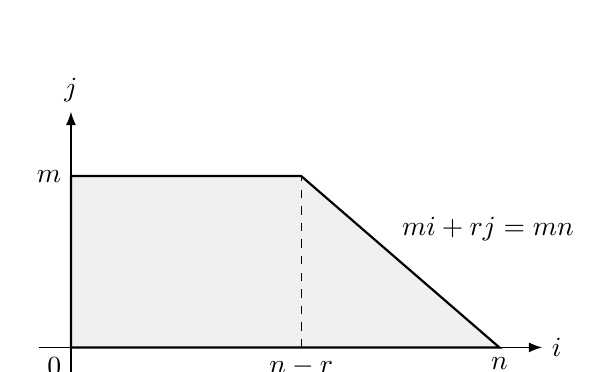
\begin{tikzpicture}[x=0.68cm,y=0.68cm,>=Latex]
\draw[->] (-0.6,0)--(8.8,0) node[right] {$i$};
\draw[->] (0,-0.6)--(0,4.4) node[above] {$j$};
\fill[black!6] (0,0)--(8,0)--(4.3,3.2)--(0,3.2)--cycle;
\draw[thick] (0,0)--(8,0)--(4.3,3.2)--(0,3.2)--cycle;
\node[below left] at (0,0) {$0$};
\node[below] at (8,0) {$n$};
\node[left] at (0,3.2) {$m$};
\draw[dashed] (4.3,0)--(4.3,3.2);
\node[below] at (4.3,0) {$n-r$};
\node[above right] at (6.0,1.8) {$mi+rj=mn$};
\end{tikzpicture}
\caption{The prescribed support. The slope parameter $r$ records how far the
upper right corner is removed. The picture is schematic.}
\label{n:fig:polygon}
\end{figure}

The upper bound records this sloping edge, rather than only the enclosing
rectangle. Put $g=\gcd(m,r)$.
\begin{thm}\label{n:thm:polygon}
For $f\in\Tcal_{m,n,r}$ the zero set of $F$ is finite and
\begin{equation}\label{n:eq:upper}
 N(F)\le\min\{n^2,\ (4m+1)n-m^2-4m-(m-1)r-g\}.
\end{equation}
\end{thm}

One endpoint of Figure~\ref{n:fig:polygon} is particularly useful. Let
$\Ecal_{m,n}$ be the entire coefficient space
\begin{equation}\label{n:eq:Eclass}
 F(z)=c z^n+
 \sum_{\substack{i,j\ge0,\ i+j\le n-1\\j\le m}}c_{ij}z^i\bar z^j,
 \qquad c\ne0.
\end{equation}
The only restriction on its top homogeneous part is that it be holomorphic;
the lower terms are neither real-valued nor harmonic in general. Denote its
largest zero count by $E_{m,n}$. This is a finite integer by
Theorem~\ref{n:thm:polygon}.

The asymptotic coefficient in this full space is sharp.
\begin{thm}\label{n:thm:E}
For $n>m\ge1$,
\begin{equation}\label{n:eq:Eupper}
 E_{m,n}\le\min\{n^2,\ (4m+1)n-2m(m+2)\}.
\end{equation}
For $n>4m+1$,
\begin{equation}\label{n:eq:Elower}
 E_{m,n}\ge(4m+1)n-4m(2m+1).
\end{equation}
The lower bound is attained by a polynomial all of whose zeros are
nondegenerate. For every fixed $m$,
\begin{equation}\label{n:eq:limit}
 \lim_{n\to\infty}\frac{E_{m,n}}n=4m+1.
\end{equation}
\end{thm}

Indeed, the lattice condition in \eqref{n:eq:support} with $r=m+1$ is exactly
\eqref{n:eq:Eclass}. For $1\le j\le m$ it is equivalent to $i+j\le n-1$;
for $j=0$ it is $i\le n$. This proves \eqref{n:eq:Eupper} from
\eqref{n:eq:upper}. The construction proving \eqref{n:eq:Elower} is given in
Section~\ref{n:sec:construction}. The gap between these two linear expressions
is $6m^2$. Thus \eqref{n:eq:limit} does not assert equality in
\eqref{n:eq:Eupper} for each pair $(m,n)$.

The other endpoint includes the total-degree class studied by S\`ete and Zur
\cite[Section~5]{SZ24}. It is substantially smaller than \eqref{n:eq:Eclass}.
\begin{cor}\label{n:cor:total}
If $\deg p=n>m\ge1$ and $\deg_{\rm tot}Q\le m$, then
\begin{equation}\label{n:eq:total}
 \#\{z:p(z)+Q(z,\bar z)=0\}
 \le\min\{n^2,\ (3m+2)n-m^2-4m-\gcd(m,n)\}.
\end{equation}
\end{cor}
\begin{proof}
Every mixed monomial in $Q$ satisfies
$mi+nj\le n(i+j)\le nm$. All analytic terms of $p$ also satisfy this
inequality. Apply Theorem~\ref{n:thm:polygon} with $r=n$.
\end{proof}

In particular, the second estimate in \eqref{n:eq:total} is not restricted to
harmonic polynomials. This extension does not identify the maximum in the
total-degree class with the harmonic maximum. Nor does the asymptotic result
\eqref{n:eq:limit} apply to that smaller class: the allowed mixed terms in
\eqref{n:eq:Eclass} can have degrees tending to $n$.

For comparison with prior work, the case of conjugate degree one is a
rational harmonic equation. Its sharper degree-dependent bounds are due to
Liesen and Zur \cite[Theorem~1.1, author version v2, p.~2]{LZ18}; sharpness
with prescribed pole multiplicities follows from Lee and Makarov
\cite[Theorem~C, p.~3]{LM14}. We record this known endpoint in
Section~\ref{n:sec:known}, rather than count it as a new result.

\subsection{Genericity within the support restriction}\label{n:sec:reg}
The inequality $r>m$ makes $cz^n$ the unique highest-total-degree term.
Lemma~\ref{d:lem:pure}, after scaling, gives finiteness and $N(F)\le n^2$.
The support in \eqref{n:eq:support} is downward closed, so
Corollary~\ref{core:regularizationspace} applies without enlarging it.
Thus we may preserve all zeros through regularization and then make a
small generic perturbation in the same support.

A sufficiently small further perturbation preserves any finite set of
nondegenerate zeros. We may consequently assume that the affine curve
$C=\{f=0\}$ is smooth and irreducible, that its finite intersections with
$\tau C$ are transverse, and that $C$ is transverse to the fixed set of
\[
 \tau(z,w)=(\bar w,\bar z).
\]
These are genuine generic conditions in the indicated sparse space.
The monomials $1,z,w$ separate first-order jets at affine points and
separate two different affine points. They give the required transversality
both off and on the fixed set. Irreducibility is a nonempty algebraic open
condition: $w^m+z^n+z$ belongs to the space and is irreducible by Eisenstein
at $z$ (the case $m=1$ is immediate). We may also assume the leading
coefficient in $w$ has simple zeros, the next coefficient is nonzero there,
and the polynomial on the sloping Newton edge has distinct nonzero roots.
These are compatible open conditions. All subsequent arguments concern
such a perturbation.

\subsection{The normalization genus}\label{n:sec:genus}
Write
\[
 f(z,w)=\sum_{j=0}^m a_j(z)w^j,
 \qquad \deg a_j\le\left\lfloor n-\frac{rj}{m}\right\rfloor.
\]
Let $\widetilde C$ be the normalization of the closure of $C$ in
$X=\CP^1_z\times\CP^1_w$, and let $\gamma$ be its genus. The projection
$z:\widetilde C\to\CP^1$ has degree $m$.

The genus can be bounded directly from the discriminant; no nonsingularity
of the curve at infinity is being assumed. Lemma~\ref{n:lem:genus} provides the
precise estimate used in the surface argument.
\begin{lem}\label{n:lem:genus}
For the generic curve just described,
\begin{equation}\label{n:eq:genus}
 2\gamma\le(2m-2)n-(m-1)r-m-g+2.
\end{equation}
Above $(\infty,\infty)$ there are exactly $g$ points of the normalization,
with local parametrizations
\begin{equation}\label{n:eq:branches}
 u=t^{m/g},\qquad v=c_\ell t^{r/g}(1+O(t)),\qquad c_\ell\ne0,
 \quad u=1/z,\ v=1/w.
\end{equation}
\end{lem}
\begin{proof}
The discriminant $\Disc_w f$ is homogeneous of degree $2m-2$ in the
coefficients $a_j$, and homogeneous of weight $m(m-1)$ when $a_j$ has
weight $j$. Therefore
\[
 \deg_z\Disc_w f\le (2m-2)n-r(m-1).
\]
When $m=1$, the discriminant is $1$ and this bound is zero.
Over a finite value of $z$ with $a_m\ne0$, its order is the total
ramification multiplicity, because the affine curve is smooth. At a zero
of $a_m$, the branch at $w=\infty$ is unramified: in $v=1/w$ the equation
is $a_m(z)+a_{m-1}(z)v+O(v^2)=0$, and both $a_m'(z)$ and $a_{m-1}(z)$
are nonzero there. The other branches are generically unramified there
as well. Thus the finite ramification contribution is at most
$(2m-2)n-r(m-1)$.

Near $(\infty,\infty)$, multiply $f(1/u,1/v)$ by $u^nv^m$.
Put $a=m/g$, $b=r/g$. Its terms of least $(a,b)$-weight form
\[
 c\prod_{\ell=1}^g(v^a-\lambda_\ell u^b),
 \qquad c\ne0,
\]
where the $\lambda_\ell$ are distinct and nonzero. All other terms have
strictly larger weight. Substituting $u=t^a$, $v=t^bV$ and dividing by the
least power of $t$ gives a polynomial in $V$ with $m$ simple nonzero roots
at $t=0$. The holomorphic implicit function theorem gives the local
expansions. Grouping the roots by the action $t\mapsto e^{2\pi i/a}t$
yields exactly $g$ branches and gives \eqref{n:eq:branches}.
There are no other points above $z=\infty$. Their total ramification is
$g(a-1)=m-g$.

Riemann--Hurwitz now gives
\[
 2\gamma-2\le-2m+(2m-2)n-r(m-1)+(m-g),
\]
which is \eqref{n:eq:genus}.
\end{proof}

The right side of \eqref{n:eq:genus} is twice the number of interior lattice
points in Figure~\ref{n:fig:polygon}. Only the displayed genus inequality is needed here.

\subsection{The quotient surface and its end}\label{n:sec:surface}
The symmetric-product map
\[
 \Phi:X\longrightarrow\operatorname{Sym}^2(\CP^1)=\CP^2,
 \qquad \Phi(z,w)=\{z,\bar w\},
\]
has fibers equal to the $\tau$-orbits. In affine coordinates it is
$[1:z+\bar w:z\bar w]$. Its restriction to the smooth affine curve is an
immersion. To check this at a fixed point, use real coordinates
$s=(z+\bar w)/2$, $t=(z-\bar w)/2$. The quotient has local form
$(s,t)\mapsto(s,t^2)$ and kernel $J(T\Fix(\tau))$. A complex tangent line
transverse to $T\Fix(\tau)$ is also transverse to its $J$-image. Away from
the fixed set the quotient is a local diffeomorphism.

The ordinary projective closures of $f=0$ and $f^*=0$ have no common point
at infinity and have degrees $n,n$. In generic position they therefore
have $n^2$ distinct affine intersections. Of these, $N(F)$ are fixed and
the rest occur in pairs. The affine image has
\begin{equation}\label{n:eq:D}
 D_+=\frac{n^2-N(F)}2
\end{equation}
ordinary double points. They are positive: the intersection of the two
complex curves is positive, transport of the second sheet by the
anti-holomorphic involution reverses its two-dimensional orientation, and
$\Phi$ reverses the ambient four-dimensional orientation. The two changes
cancel. There are no triple points, since fibers have size at most two.

If $\alpha,\beta$ are the positive cohomology generators of the two factors
and $H$ is the hyperplane class, then $\Phi^*H=\alpha-\beta$. The coordinate
projections on $\widetilde C$ have degrees $m,n$. Thus the image homology
class has degree $m-n$. Reversing the source orientation makes it positive,
of degree $d=n-m$. This reversal does not change double-point signs.

The finite points of $C$ on $w=\infty$ are smooth, unramified points with
distinct images. Their partners under $\tau$ are not on $C$, since $C$
has no point with $z=\infty,w\ne\infty$. They introduce no additional
double points. It remains to treat $(\infty,\infty)$.

The required filling is elementary at the level of parametrized complex
curves. We spell out why its double points have the correct sign.
\begin{lem}\label{n:lem:cap}
The mirror torus link $T(a,-b)$, with $a,b>0$, bounds
$\gcd(a,b)$ immersed oriented disks in a four-ball, with only negative
ordinary double points.
\end{lem}
\begin{proof}
The normalization of the complex curve $Y^a=X^b$ in a small ball is a
union of $e=\gcd(a,b)$ disks, parametrized by
$(X,Y)=(t^{a/e},\zeta_\ell t^{b/e})$. Perturb these parametrizations by
sufficiently small holomorphic polynomial maps. Generic such perturbations
have nonzero derivative, only transverse double intersections, and no
triple intersections. This follows from jet transversality: polynomial
variations of sufficiently large degree interpolate the first jets at one
point and the values at two or three distinct points. The respective bad
conditions have the required real codimensions $4,4,8$.
All transverse intersections are positive because the disks are complex
curves. Near the boundary the unperturbed maps are embedded and transverse
to the sphere; their perturbed inverse images of the ball remain disks and
the boundary link remains isotopic to $T(a,b)$.
Reflect one complex coordinate of the ambient ball. It reverses its
orientation, turns every double point negative, and mirrors the boundary
link. A collar realizing the boundary isotopy gives the claimed filling.
\end{proof}

We next identify the actual link, including a Newton edge with more than two
monomials. Put $a=m/g$, $b=r/g$, so $b>a$. Near $\Phi(\infty,\infty)$
use coordinates
\[
 X=u+\bar v,\qquad Y=u\bar v.
\]
By \eqref{n:eq:branches}, $|v|=o(|u|)$ and $X=u(1+o(1))$.
For the branch associated with $\lambda_\ell$ the boundary on $|X|=\rho$
satisfies, after $Y=\rho^{1+b/a}\eta$,
\begin{equation}\label{n:eq:braid}
 \eta^a=\overline{\lambda_\ell}e^{-i(b-a)\theta}+o(1),
 \qquad X=\rho e^{i\theta}.
\end{equation}
The convergence is in $C^1$ in the angular parametrizations. The roots of
the limiting equations are distinct and nonzero, so the small error in
\eqref{n:eq:braid} does not alter the braid type.

Move the $g$ distinct nonzero constants $\overline{\lambda_\ell}$ through
a path of distinct nonzero configurations to a scaled set of $g$th roots
of unity. The displayed roots never collide, so this gives a link isotopy.
The resulting union is
\[
 \eta^m=C e^{-i(r-m)\theta},\qquad C\ne0,
\]
which is $T(m,-(r-m))$. It has $\gcd(m,r-m)=g$ components, in agreement
with the $g$ normalization disks. A rounded bidisk in the $(X,Y)$ chart
is a four-ball whose boundary contains this braid; by taking $\rho$ small,
the curve meets its boundary only on this part. Formula
\eqref{n:eq:branches} also shows that its inverse image consists of $g$
disks. Their induced orientations agree with the complex-parameter
orientations of the mirrored torus link. If the whole source is reversed,
reverse the orientations of all filling disks as well.

Replace these disks by the fillings in Lemma~\ref{n:lem:cap}, matching collars
by the link isotopy. No source handle is introduced, all new double points
are negative, and a replacement inside a ball does not change the global
homology class. We obtain a closed connected immersed surface of genus
$\gamma$, degree $d=n-m$, and exactly the positive double points in
\eqref{n:eq:D}.

We use the immersed Thom inequality in the following precise form:
\begin{equation}\label{n:eq:thom}
 \gamma+D_+\ge\frac{(d-1)(d-2)}2.
\end{equation}
The version allowing only negative double points is stated in Orevkov
\cite[Theorem~3.1, author version v2, p.~8]{Ore24}, with attribution to
Kronheimer--Mrowka \cite{KM94}. Resolving each positive double point by an
oriented annulus increases the genus by one, leaves the homology class
unchanged, and reduces the general case to that version. Thus it is
\eqref{n:eq:thom}, not an inequality for a singular image, that applies.

Combining \eqref{n:eq:genus}, \eqref{n:eq:D}, and \eqref{n:eq:thom} yields
\[
 N(F)\le n^2+(2m-2)n-(m-1)r-m-g+2
       -(n-m-1)(n-m-2).
\]
The expression simplifies to the second bound in \eqref{n:eq:upper}.
Lemma~\ref{core:regularizationspace} and the preservation of nondegenerate zeros under the
subsequent small perturbation transfer it to every initial polynomial.
This proves Theorem~\ref{n:thm:polygon}.

\subsection{An exact count of zeros approaching infinity}\label{n:sec:infinity}
Adding a higher analytic monomial changes both the leading homogeneous part
and the degree at infinity. In the following situation every added zero
can be counted, without an uncontrolled intermediate scale.
\begin{lem}\label{n:lem:infinity}
Let $k>m\ge1$, $r>m$, and let $P\in\C[z,w]$ have degrees at most $k,m$
in $z,w$, respectively, with $[z^kw^m]P=c\ne0$. Suppose all zeros of
$P(z,\bar z)$ are nondegenerate. For all sufficiently small real
$\varepsilon>0$, the polynomial
\[
 F_\varepsilon(z)=P(z,\bar z)+\varepsilon z^{k+r}
\]
has exactly $N(P(z,\bar z))+r+m$ zeros, all nondegenerate. The $r+m$ new
zeros approach infinity and have positive Jacobian.
\end{lem}
\begin{proof}
The term $cz^kw^m$ is the unique term of total degree $k+m$. All old zeros
are confined to a compact set, and each persists uniquely under the small
perturbation. Set $t=\varepsilon^{1/(r-m)}$ and $z=\zeta/t$. On compact
$\zeta$-sets,
\begin{equation}\label{n:eq:scaling}
 t^{k+m}F_\varepsilon(\zeta/t)
 =\zeta^k(\zeta^r+c\bar\zeta^m)+O(t),
\end{equation}
with $C^1$ convergence. The nonzero zeros of the limit satisfy
\[
 |\zeta|^{r-m}=|c|,
 \qquad (r+m)\arg\zeta=\arg(-c)\pmod{2\pi}.
\]
There are exactly $r+m$. At such a zero the Jacobian of
$\zeta^r+c\bar\zeta^m$ is
\[
 (r^2-m^2)|\zeta|^{2r-2}>0.
\]
Multiplication by $\zeta^k$ preserves its sign. The implicit function theorem
applied to \eqref{n:eq:scaling} gives one simple positive zero near each.

For completeness, choose $R$ so large that
\[
 |P(z,\bar z)-cz^k\bar z^m|
 \le \tfrac12|c|\,|z|^{k+m}\quad (|z|\ge R).
\]
Any zero of $F_\varepsilon$ there must satisfy
\[
 \tfrac12|c|\le \varepsilon|z|^{r-m}\le\tfrac32|c|.
\]
Its scaled coordinate $\zeta=tz$ therefore lies in a fixed compact annulus.
Every limit point in that annulus is one of the above $r+m$ simple zeros;
compactness and local uniqueness exclude further zeros there.
On $|z|\le R$, compactness away from disjoint old-zero neighborhoods excludes
all other zeros for small $\varepsilon$. This proves the exact count.
\end{proof}

The lemma applies to the full rectangle of exponents $i\le k,j\le m$.
After adding $z^{k+r}$, this rectangle and the new exponent all belong to
\eqref{n:eq:support} with $n=k+r$, because $mi+rj\le mk+rm=mn$.


\subsection{The optimal coefficient in the support-restricted space}\label{n:sec:construction}
The radial polynomial in Proposition~\ref{b:prop:radial}, with analytic
degree $k>3m$, has $(4m+1)(k-m)$ nondegenerate zeros and a nonzero
coefficient at $z^kw^m$. Its coefficients may be chosen real rational.
We combine it with the preceding exact count at infinity.

Denote the largest zero count in $\Tcal_{m,n,r}$ by $K_{m,n,r}$.
The combination of the preceding lemmas proves a slightly more general
asymptotic statement than Theorem~\ref{n:thm:E}.
\begin{prop}\label{n:prop:lower}
If $n>r+3m$ and $r>m$, then
\begin{equation}\label{n:eq:Klower}
 K_{m,n,r}\ge(4m+1)n-4m(r+m).
\end{equation}
For fixed $m,r$ with $r>m$, $\lim_{n\to\infty}K_{m,n,r}/n=4m+1$.
\end{prop}
\begin{proof}
Put $k=n-r>3m$. Lemma~\ref{b:prop:radial} gives $(4m+1)(k-m)$ zeros.
Lemma~\ref{n:lem:infinity} adds exactly $r+m$, giving
\[
 (4m+1)(n-r-m)+(r+m)=(4m+1)n-4m(r+m).
\]
The resulting polynomial lies in $\Tcal_{m,n,r}$ by the observation at the
end of Section~\ref{n:sec:infinity}. This proves \eqref{n:eq:Klower}; dividing
it and \eqref{n:eq:upper} by $n$ proves the limit.
\end{proof}

For $r=m+1$ this gives \eqref{n:eq:Elower}. Together with
\eqref{n:eq:Eupper}, it proves \eqref{n:eq:limit} and completes
Theorem~\ref{n:thm:E}. All constructed zeros are nondegenerate, and the final
$\varepsilon$ can be chosen positive rational.

The distinction between the two support restrictions is substantive.
For example, when $m\ge2$ is fixed, Corollary~\ref{n:cor:total} bounds the
leading coefficient for $p+Q$ with $\deg_{\rm tot}Q\le m$ by $3m+2$,
whereas Theorem~\ref{n:thm:E} gives the strictly larger optimal coefficient
$4m+1$ in \eqref{n:eq:Eclass}. Both classes have holomorphic highest
homogeneous term. That condition alone is therefore insufficient to
obtain the lower coefficient.

\subsection{A known sharp endpoint and the remaining gap}\label{n:sec:known}
There is a complete degree-dependent answer when $m=1$. We include it to
locate the new bounds relative to established sharp results.
\begin{prop}\label{n:prop:known}
For $2\le r\le n$,
\begin{equation}\label{n:eq:known}
 K_{1,n,r}=5n-2r-2.
\end{equation}
In particular, $E_{1,n}=5n-6$ for every $n\ge2$.
\end{prop}
\begin{proof}
Write $f=p(z)-wq(z)$, with $\deg p=n$, $\deg q\le n-r$.
If $q\equiv0$, the elementary analytic bound suffices. Otherwise, remove
a greatest common divisor of degree $s$, leaving numerator and denominator
degrees $a=n-s$ and $b\le n-r-s$. The rational harmonic bound in
\cite[Theorem~1.1, author version v2, p.~2]{LZ18} gives
\[
 N(f(z,\bar z))\le s+3a+2b-2\le5n-2r-2.
\]
Here $a-b\ge r\ge2$; denominator zeros are not rational zeros because the
reduced pair is coprime.

For equality, apply Lee--Makarov's Theorem~C
\cite[p.~3]{LM14} with rational degree $n$, one pole of order $r$ at
infinity, and $n-r$ simple finite poles. There are $n-r+1$ distinct poles.
Their theorem gives
\[
 \min\{3n+2(n-r+1)-3,5n-5\}=5n-2r-1
\]
fixed points on the sphere. Infinity is one, leaving $5n-2r-2$ finite
zeros. The numerator and denominator degrees are $n,n-r$.
Regularity of an extremizer also follows from
\cite[Theorem~3.5, author version v2, p.~7]{LZ18}.
Taking $r=2$ proves the last assertion.
\end{proof}

Proposition~\ref{n:prop:known} is already implicit in those results and is not
claimed here as new. It also shows that the upper bound in
Theorem~\ref{n:thm:polygon} is not always the finite-degree maximum: for
$m=1,r>2$ it gives $5n-6$, whereas \eqref{n:eq:known} is smaller.

The finite-degree equalities proved later in Theorem~\ref{d:thm:main}
settle part of this range. The general expression in
Theorem~\ref{n:thm:polygon} is an upper bound, not a claim of equality
for every triple $(m,n,r)$.

\section{A bound depending on the total-degree gap}\label{g:sec:gap}
Let $1\le m<n$, let $p\in\C[z]$ have degree $n$, and let
$Q\in\C[z,w]$ have total degree at most $m$. We write
\begin{equation}\label{g:eq:F}
 F(z)=p(z)+Q(z,\bar z),\qquad d=n-m,\qquad
 N(F)=\#\{z\in\C:F(z)=0\}.
\end{equation}
In this note the first variable of $Q$ is the analytic variable. The
restriction on $Q$ is a \emph{total-degree} restriction, not merely a bound
on its degree in $w$. Thus the class in \eqref{g:eq:F} contains every harmonic
polynomial $p+\overline q$ with $\deg q\le m$, but it does not contain all
polyanalytic polynomials of bidegree $(m,n)$.

The classical harmonic estimate is $n^2$; see Wilmshurst
\cite[pp.~2077--2079]{Wil98}. The Hermitian trace approach developed by
Furch\`i gives $n^2-2$ when $m\le n-2$, subject in his statement to a possible
$n^2-1$ exception determined by two analytic coefficients
\cite[Theorem~1.1, author version v2, p.~2]{Fur25}.
The proof below removes that exception and permits mixed lower-degree terms. The estimate below takes account of
the entire gap between the two degrees.

This is the main result of the present note.
\begin{thm}\label{g:thm:main}
Under the assumptions in \eqref{g:eq:F}, the zero set of $F$ is finite and
\begin{equation}\label{g:eq:bound}
 N(F)\le n^2-2\left\lfloor\frac{(n-m)^2}{4}\right\rfloor.
\end{equation}
\end{thm}

For $d=2$, \eqref{g:eq:bound} is $n^2-2$. For $d=3,4,5,6$ the deficits from
$n^2$ become $4,8,12,18$, respectively. For large $n$ with $m$ fixed, this is
still a quadratic estimate; it is not a replacement for the linear bound
of Corollary~\ref{n:cor:total}. Rather, the two bounds are effective in different regimes.
No claim of sharpness for every $d$ is made.

The proof uses the standard Hermitian trace form, whose signature counts
real solutions in the appropriate real structure. That correspondence is
Furch\`i's Theorem~3.13 and Corollary~3.14
\cite[author version v2, pp.~9--10]{Fur25}; we include the required argument,
including multiple complex roots. The additional ingredient is a totally
isotropic subspace of dimension $\lfloor d^2/4\rfloor$. 
\subsection{The quotient algebra and its Hermitian form}
Divide $F$ by the leading coefficient of $p$, so that $p$ is monic.
For a univariate polynomial $a$, put
$a^\#(w)=\overline{a(\bar w)}$. For $a\in\C[z,w]$, put
\[
 a^*(z,w)=\overline{a(\bar w,\bar z)}.
\]
The latter is a conjugate-linear involution. Define
\begin{equation}\label{g:eq:algebra}
 f=p(z)+Q(z,w),\qquad
 f^*=p^\#(w)+Q^*(z,w),\qquad
 \A=\C[z,w]/(f,f^*).
\end{equation}
With any graded monomial order, the leading monomials of $f$ and $f^*$ are
$z^n$ and $w^n$. Since these are relatively prime, the two polynomials form
a Gr\"obner basis. Consequently
\begin{equation}\label{g:eq:basis}
 \{z^i w^j:0\le i,j<n\}
\end{equation}
is a basis of $\A$ and $\dim_\C\A=n^2$. This proves, in particular, the
finiteness assertion in Theorem~\ref{g:thm:main}. We identify a polynomial
with its class when no ambiguity can arise.

For $a\in\A$, let $M_a$ denote multiplication by $a$, and set
\begin{equation}\label{g:eq:form}
 T(a)=\Tr M_a,\qquad \HH(a,b)=T(ab^*).
\end{equation}
The ideal in \eqref{g:eq:algebra} is invariant under $*$, so these expressions
are well defined. Moreover $T(a^*)=\overline{T(a)}$; hence $\HH$ is Hermitian.
The involution satisfies
$\HH(a^*,b^*)=\overline{\HH(a,b)}$.

The signature is the positive index minus the negative index; the radical
is the nullspace. The following form of the signature theorem retains
all multiplicities throughout the algebraic argument.
\begin{lem}\label{g:lem:signature}
The signature of $\HH$ is $N(F)$. If $R$ is the number of distinct common
zeros of $f,f^*$ and $s$ is the number of two-element orbits of
$(z,w)\mapsto(\bar w,\bar z)$ on this set, then
\[
 \rank\HH=R,\qquad \nu_-(\HH)=s,\qquad
 N(F)=R-2s.
\]
Here $\nu_-$ denotes the number of negative eigenvalues, counted with
multiplicity.
\end{lem}
\begin{proof}
Decompose the finite algebra into its local algebras. On a local algebra
of length $\mu$ supported at $x$, multiplication by $a$ has trace
$\mu a(x)$: the difference from scalar multiplication is nilpotent.
At a fixed point of the involution the resulting trace form has a single
positive eigenvalue, with coefficient $\mu$, and is zero on the maximal
ideal. At a nonfixed pair $x,x^*$, the two local lengths agree; on their
constant coordinates the matrix of the form is
\[
 \begin{pmatrix}0&\mu\\ \mu&0\end{pmatrix}.
\]
It has one positive and one negative eigenvalue. The remaining local
coordinates are in the radical. Different orbits are orthogonal. Adding
these contributions proves the assertions and identifies the fixed
points with the zeros of $F$.
\end{proof}

A single isotropic subspace can lose dimension in the radical. The
involution provides precisely the control needed to handle this loss.
\begin{lem}\label{g:lem:isotropic}
Let $V$ be a finite-dimensional complex vector space with a Hermitian form
$H$ and a conjugate-linear involution $J$ satisfying
$H(Ju,Jv)=\overline{H(u,v)}$. If $U\subset V$ is totally isotropic and
$U\cap JU=\{0\}$, then
\begin{equation}\label{g:eq:signaturebound}
 \operatorname{signature}H\le \dim V-2\dim U.
\end{equation}
\end{lem}
\begin{proof}
Put $r=\dim\rad H$ and $k=\dim(U\cap\rad H)$. The radical is $J$-invariant.
The subspaces $U\cap\rad H$ and $J(U\cap\rad H)$ are disjoint, so $r\ge2k$.
In the nondegenerate quotient $V/\rad H$, the image of $U$ is isotropic of
dimension $\dim U-k$. Projection onto the negative eigenspace is injective
on any isotropic subspace of a nondegenerate Hermitian space. Therefore
$\nu_-(H)\ge\dim U-k$. It follows that
\[
 \operatorname{signature}H
 =\dim V-r-2\nu_-(H)
 \le\dim V-2\dim U-r+2k
 \le\dim V-2\dim U,
\]
as required.
\end{proof}

We shall apply \eqref{g:eq:signaturebound} to \eqref{g:eq:form}. No simplicity
assumption on the roots of the complexified system will be needed.

\subsection{An exact trace identity below degree \texorpdfstring{$2d$}{2d}}
Write
\[
 Q(z,w)=\sum_{r+s\le m}c_{rs}z^rw^s.
\]
For a univariate polynomial $u$, let
\[
 S(u)=\Tr_{\C[z]/(p)} M_u,
 \qquad
 D_r(u)=[z^{n-1}]\bigl(z^ru'(z)\bmod p(z)\bigr).
\]
The remainder in this definition has degree less than $n$. Use
$S^\#,D_r^\#$ for the corresponding functionals defined by $p^\#$ in the
variable $w$. These are complex-linear functionals. In particular,
\begin{equation}\label{g:eq:Dvanish}
 D_r(u)=0\quad\hbox{if }\deg u+r<n,
\end{equation}
and the same assertion holds for $D_r^\#$. Also
$S^\#(u^\#)=\overline{S(u)}$.

The next identity, rather than just a single vanishing trace, is the
algebraic input to the proof.
\begin{lem}\label{g:lem:traceidentity}
If $u\in\C[z]$, $v\in\C[w]$, and $\deg u+\deg v<2d$, then
\begin{equation}\label{g:eq:traceidentity}
\begin{split}
 T(u(z)v(w))={}&S(u)S^\#(v)\\
 &-\sum_{r+s\le m}c_{rs}D_r(u)S^\#(w^s v)\\
 &-\sum_{r+s\le m}\bar c_{rs}S(z^s u)D_r^\#(v).
\end{split}
\end{equation}
\end{lem}
\begin{proof}
Introduce a real parameter $t$ and replace $Q,Q^*$ by $tQ,tQ^*$ in
\eqref{g:eq:algebra}; denote the multiplication trace by $T_t$. The standard
basis \eqref{g:eq:basis} is unchanged for every $t$.

We first show that $T_t(z^a w^b)$ is affine in $t$ when $a+b<2d$.
To compute a diagonal entry of the multiplication matrix, reduce
$z^{a+i}w^{b+j}$ to standard monomials. A substitution using a lower term
of $p$ or $p^\#$ decreases total degree by at least one. A substitution
using a term of $tQ$ or $tQ^*$ decreases total degree by at least $n-m=d$
and contributes one factor of $t$. A reduction path ending in $z^iw^j$
can decrease degree by only $a+b$. It therefore uses at most one term
containing $t$. All reductions strictly decrease total degree, so they
terminate, and each diagonal entry is affine in $t$. Linearity gives the
same assertion for $T_t(uv)$.

Suppose first that $p$ has distinct roots $\alpha_1,\ldots,\alpha_n$.
At $t=0$, the roots of the complexified system are the simple grid points
$(\alpha_a,\bar\alpha_b)$. Their derivatives satisfy
\[
 z'_{ab}(0)=-\frac{Q(\alpha_a,\bar\alpha_b)}{p'(\alpha_a)},\qquad
 w'_{ab}(0)=-\frac{Q^*(\alpha_a,\bar\alpha_b)}{(p^\#)'(\bar\alpha_b)}.
\]
For small $t$, the trace is the sum of the values of $uv$ at these
$n^2$ simple roots. Differentiating this sum at zero gives
\eqref{g:eq:traceidentity}, because Lagrange interpolation yields
\begin{equation}\label{g:eq:lagrange}
 D_r(u)=\sum_{a=1}^n
 \frac{\alpha_a^r u'(\alpha_a)}{p'(\alpha_a)}.
\end{equation}
Indeed, the right side is the coefficient of $z^{n-1}$ in the remainder of
$z^ru'$ modulo $p$. The constant term in $t$ is $S(u)S^\#(v)$, and the two
sums in \eqref{g:eq:traceidentity} are its first derivative. Affineness in $t$
makes this first-order identity exact at $t=1$.

Finally, all expressions in \eqref{g:eq:traceidentity}, with $D_r$ defined by
remainders, are polynomial functions of the coefficients of $p,Q$ and
their conjugates. The identity therefore extends from polynomials $p$ with
simple roots to all monic $p$. Formula~\eqref{g:eq:lagrange} is used only in
the proof on the dense simple-root locus.
\end{proof}

The threshold $2d$ is important. At total degree $2d$, two substitutions
using the perturbation can contribute to a diagonal entry, and the trace
need not be affine in $Q$. We do not use \eqref{g:eq:traceidentity} at that
threshold or beyond it.

\subsection{A large isotropic subspace}
For the moment assume that the leading moment matrices
\begin{equation}\label{g:eq:momentcondition}
 \bigl(S(z^{a+b})\bigr)_{0\le a,b\le k},\qquad 0\le k<d,
\end{equation}
are nonsingular. This is a nonempty Zariski-open condition on the
coefficients of $p$. To see nonemptiness, take $p$ with $n$ distinct real
roots: the matrices are positive definite for $k<n$, by evaluation of a
nonzero real polynomial of degree at most $k$ at those roots.

Apply Gram--Schmidt to $1,z,\ldots,z^{d-1}$ for the complex bilinear pairing
$(a,b)\mapsto S(ab)$. The result is a sequence of monic polynomials
$r_i$ of degree $i$, satisfying
\begin{equation}\label{g:eq:orthogonality}
 S(r_i a)=0\quad(\deg a<i),\qquad 0\le i<d.
\end{equation}
This is bilinear orthogonality, not Hermitian orthogonality. Positivity is
not assumed for the general complex polynomial $p$.

We can now construct the subspace needed in Lemma~\ref{g:lem:isotropic}.
\begin{prop}\label{g:prop:U}
Under \eqref{g:eq:momentcondition}, the subspace
\begin{equation}\label{g:eq:U}
 U=\spanC\{r_i(z)r_j^\#(w):0\le j<i,\ i+j\le d-1\}\subset\A
\end{equation}
is totally isotropic for $\HH$, satisfies $U\cap U^*=\{0\}$, and has
complex dimension $\lfloor d^2/4\rfloor$.
\end{prop}
\begin{proof}
The products $r_i(z)r_j^\#(w)$ with $0\le i,j<d$ are linearly independent
in \eqref{g:eq:basis}. The involution exchanges their two indices.
The index sets defining $U$ and $U^*$ are disjoint, which proves
$U\cap U^*=\{0\}$. Counting the pairs with $i>j$ and $i+j\le d-1$ gives
\begin{equation}\label{g:eq:dimension}
 \dim U=
 \begin{cases}
 t^2,&d=2t,\\
 t(t+1),&d=2t+1,
 \end{cases}
 =\lfloor d^2/4\rfloor.
\end{equation}

Take indices $(i,j),(k,\ell)$ occurring in \eqref{g:eq:U} and put
\[
 u=r_i r_\ell,\qquad v=r_j^\# r_k^\#.
\]
Their total degree is at most $2d-2$, so Lemma~\ref{g:lem:traceidentity}
applies. The constant term $S(r_i r_\ell)S^\#(r_j^\#r_k^\#)$ is zero:
by \eqref{g:eq:orthogonality}, both factors could be nonzero only if
$i=\ell$ and $j=k$, contradicting $i>j$ and $k>\ell$.

Consider a term with coefficient $c_{rs}$ in the first sum of
\eqref{g:eq:traceidentity}. If $D_r(u)\ne0$, then \eqref{g:eq:Dvanish} implies
$i+\ell+r\ge n$. Since $i+j\le n-m-1$, it follows that
\[
 \ell-j\ge m+1-r,\qquad k-j\ge m+2-r>s.
\]
Thus $j+s<k$, and \eqref{g:eq:orthogonality} implies
$S^\#(w^s r_j^\# r_k^\#)=0$. If $D_r(u)=0$, the same term is zero directly.
Hence every term in the first sum vanishes.

For the second sum, a nonzero $D_r^\#(v)$ would imply $j+k+r\ge n$.
Using $k+\ell\le n-m-1$ and $i>j$, we obtain
\[
 j-\ell\ge m+1-r,\qquad i-\ell\ge m+2-r>s.
\]
Now $\ell+s<i$, so $S(z^s r_i r_\ell)=0$. Every term in the second sum
also vanishes. By \eqref{g:eq:form}, the resulting identity $T(uv)=0$ is
precisely the required pairwise isotropy of $U$.
\end{proof}

Combining Lemmas~\ref{g:lem:signature} and~\ref{g:lem:isotropic} with
Proposition~\ref{g:prop:U}, including \eqref{g:eq:dimension}, proves \eqref{g:eq:bound} under
\eqref{g:eq:momentcondition}. Notice that the common zeros of $f,f^*$ may
have arbitrary multiplicities: the radical estimate in
Lemma~\ref{g:lem:isotropic} has already accounted for them.


\subsection{Removing the auxiliary moment condition}
We finish the proof of Theorem~\ref{g:thm:main}. The coefficient space
$p(z)+Q(z,w)$, $\deg p\le n$, $\deg_{\rm tot}Q\le m$, is stable under
both derivatives. The highest analytic coefficient remains nonzero.
Corollary~\ref{core:regularizationspace} therefore gives an arbitrarily
small perturbation in this space, without decreasing the zero count,
whose zeros are all nondegenerate. A further small change of the
coefficients of $p$ preserves these zeros and satisfies the nonempty
Zariski-open moment condition \eqref{g:eq:momentcondition}. The estimate
proved using Proposition~\ref{g:prop:U} applies to that last polynomial,
and hence to the original one. This proves \eqref{g:eq:bound} with no
assumption on multiplicities or moment matrices.

For a gap of two the bound is $n^2-2$, and it is attained by the
real-valued construction in Theorem~\ref{r:thm:main}, with $m=n-2$.
Consequently the total-degree statement from the earlier drafts is
retained in its strongest form: for $\deg p=n\ge3$ and
$\deg_{\rm tot}Q\le n-2$, the maximum is exactly $n^2-2$.
For larger gaps the formula \eqref{g:eq:bound} is an upper bound,
not an asserted sharp formula. Combining it with
\eqref{n:eq:total} gives the two upper bounds in
Theorem~\ref{core:harmonicbounds} for the harmonic subclass.

\section{Harmonic polynomials with many zeros}\label{b:sec:harmonic}

We now turn to \eqref{b:eq:harmonicfamily}. Unlike the examples in
Section~\ref{b:sec:radial}, every polynomial constructed in this
section is harmonic. The upper bound refines the Descartes argument
of \cite[Section~4.1, \av, pp.~8--9]{Lun23}; the lower bound makes
that argument exact on every line at once. The coefficients on
different lines are not independent, and we keep track of their
common angular dependence throughout.

The full harmonic maximum also equals the maximal valence in that class,
since subtracting a constant preserves both degrees.

Lundberg's probabilistic construction gives
$M^{\mathrm{harm}}_{m,n}\ge\lceil n\sqrt m\rceil$ by using the family
\begin{equation}\label{b:eq:harmonicfamily}
 h(z)=\varepsilon z^n+q(z)+\overline{q(z)},\qquad
 \deg q=m<n,\quad \varepsilon\in\C\setminus\{0\}.
\end{equation}
His concluding question asks for a deterministic choice of $q$ giving
$mn$-order many zeros in this same family
\cite[Section~4.2, \av, p.~9]{Lun23}.
We determine its exact maximal zero count, denoted by $S_{m,n}$.
Put $g=\gcd(m,n)$ and define
\begin{equation}\label{b:eq:harmonicdelta}
 \Delta_{m,n}=
 \begin{cases}
  g,&\text{if $m/g$ and $n/g$ are both odd},\\
  0,&\text{otherwise}.
 \end{cases}
\end{equation}
The correction in \eqref{b:eq:harmonicdelta} comes from the parity of
the exponent gap and a count of equally spaced directions.
\begin{thm}\label{b:thm:harmonic}
For every $1\le m<n$,
\begin{equation}\label{b:eq:harmonicexact}
 S_{m,n}=n(m+1)+\Delta_{m,n}.
\end{equation}
The maximum is attained with $\varepsilon\in\Q_{>0}$ and
$q\in\Q(i)[z]$, and all zeros of the extremizer are nondegenerate.
\end{thm}

\subsection{Real restrictions and the last exponent gap}
For real polynomials the contribution of the final gap can be
bounded more precisely than by two in all cases.
\begin{lem}\label{b:lem:harmonicgap}
Let $N>M\ge0$, let $a\in\R\setminus\{0\}$, and let
$u\in\R[r]$ have degree at most $M$. Write $b=[r^M]u$ for the
coefficient of $r^M$. The number of nonzero real roots of
$ar^N+u(r)$, counted with multiplicity, is at most
\[
 \begin{cases}
  M+1,&N-M\text{ odd},\\
  M+2\mathbf1_{\{ab<0\}},&N-M\text{ even},
 \end{cases}
\]
where the indicator $\mathbf1_{\{ab<0\}}$ equals one when $ab<0$
and zero otherwise.
\end{lem}
\begin{proof}
There is nothing to prove if $u=0$. Otherwise, put $d=\deg u$ and
list its nonzero coefficients in increasing exponent order.
An odd gap between successive exponents contributes exactly one
sign change in total to the coefficient lists of $u(r)$ and
$u(-r)$. An even gap contributes zero or two sign changes, which
is at most its size. The total contribution within $u$ is
therefore at most $d$.

Appending the degree-$N$ coefficient contributes one when $N-d$
is odd. When $N-d$ is even, it contributes two precisely if the
two leading coefficients have opposite signs, and otherwise zero.
If $d=M$, this proves the assertion by Descartes' rule on the two
half-lines. If $d<M$ and $N-M$ is odd, use $d+2\le M+1$.
If $N-M$ is even, the case $d=M-1$ has odd last gap and gives
$d+1=M$; for $d\le M-2$, use $d+2\le M$. These last two cases
also explain why a vanishing coefficient $b$ causes no exception.
\end{proof}

A rotation $z=e^{i\theta}\zeta$ with
$\varepsilon e^{in\theta}>0$ reduces \eqref{b:eq:harmonicfamily} to
$\varepsilon>0$. The transformed polynomial $q(e^{i\theta}\zeta)$
still has degree $m$. After this normalization, the imaginary part
of $h$ vanishes exactly on the lines
\begin{equation}\label{b:eq:harmoniclines}
 \Lambda_j=e^{ij\pi/n}\R,\qquad 0\le j<n.
\end{equation}
Write $q(z)=\sum_{k=0}^m a_kz^k$, with $a_m\ne0$, and put
$\theta_j=j\pi/n$. The restriction to $\Lambda_j$ is the real
polynomial
\begin{equation}\label{b:eq:harmonicrestriction}
 f_j(r)=\varepsilon(-1)^jr^n+
             2\sum_{k=0}^m\Rea(a_ke^{ik\theta_j})r^k.
\end{equation}
Its leading coefficient never vanishes. In particular, every member
of \eqref{b:eq:harmonicfamily} has a finite zero set, and the possible
integer counts are bounded. Thus the maximum defining $S_{m,n}$
exists.

\subsection{The exact upper bound}
Assume first that $\Rea a_0\ne0$. The origin is not a zero, so
counts on the distinct lines \eqref{b:eq:harmoniclines} may be added.
If $n-m$ is odd, Lemma~\ref{b:lem:harmonicgap} gives at most $m+1$
roots per line. The resulting bound is $n(m+1)$, and in this case
$\Delta_{m,n}=0$.

Suppose that $n-m=2d$ is even, and put
\[
 G=\gcd(n,d),\qquad \ell=n/G,\qquad a_m=|a_m|e^{i\beta}.
\]
The sign controlling the final gap in
\eqref{b:eq:harmonicrestriction} is that of
\[
 (-1)^j\Rea(a_me^{imj\pi/n})
 =|a_m|\cos\left(\beta-\frac{2\pi dj}{n}\right).
\]
By Lemma~\ref{b:lem:harmonicgap},
\begin{equation}\label{b:eq:harmonicangular}
 N(h)\le nm+2B_\beta,\qquad
 B_\beta=\#\left\{0\le j<n:
       \cos\left(\beta-\frac{2\pi dj}{n}\right)<0\right\}.
\end{equation}
As $j$ varies, the angles $2\pi dj/n$ traverse the vertices of a
regular $\ell$-gon, each with multiplicity $G$.
An open semicircle contains at most $\ell/2$ such vertices when
$\ell$ is even and at most $(\ell+1)/2$ when $\ell$ is odd.
The first assertion follows by pairing antipodal vertices. For the
second, $(\ell+3)/2$ consecutive vertices would span an angle
$\pi+\pi/\ell$, which is longer than a semicircle. Therefore
\begin{equation}\label{b:eq:harmonicsemicircle}
 2B_\beta\le
 \begin{cases}
  n,&\ell\text{ even},\\
  n+G,&\ell\text{ odd}.
 \end{cases}
\end{equation}
Boundary vertices have zero cosine and are not counted, so no
nonvanishing assumption on the intermediate coefficients is used.

We identify the parity alternative in \eqref{b:eq:harmonicsemicircle}
with \eqref{b:eq:harmonicdelta}. Write $m=gu$ and $n=gv$, where
$g=\gcd(m,n)$ and $\gcd(u,v)=1$. If $u,v$ are both odd, then
\[
 G=\gcd\bigl(gv,g(v-u)/2\bigr)=g,\qquad \ell=v\text{ is odd}.
\]
Here $\gcd(v,(v-u)/2)=1$ because $v$ is odd and coprime to $u$.
Otherwise $u,v$ have opposite parity. Since $n-m=g(v-u)$ is even,
$g$ is even, and
\[
 G=\frac g2\gcd(2v,v-u)=\frac g2,\qquad \ell=2v\text{ is even}.
\]
The last greatest common divisor is one because $v-u$ is odd and
coprime to $v$. Equations~\eqref{b:eq:harmonicangular} and
\eqref{b:eq:harmonicsemicircle} now give
$N(h)\le n(m+1)+\Delta_{m,n}$.

It remains to treat $\Rea a_0=0$. Each $f_j$ in
\eqref{b:eq:harmonicrestriction} is then divisible by $r$.
Apply Lemma~\ref{b:lem:harmonicgap} to $f_j/r$, using
$(N,M)=(n-1,m-1)$. The last-gap parity and the two relevant leading
signs are unchanged, whereas each nonzero-root bound decreases by
one. The common origin must be restored once, not $n$ times. This
actually gives the stronger estimate
\[
 N(h)\le n(m+1)+\Delta_{m,n}-n+1.
\]
The upper bound in Theorem~\ref{b:thm:harmonic} is therefore valid for
all members of the family, including those with a zero at the
origin, missing coefficients, or degenerate zeros.

\subsection{Rational coefficients attaining the bound}
The lower bound uses the same lines but forces every restriction to
attain its Descartes bound. Fix $m<n$ and set
\begin{equation}\label{b:eq:harmonicparameters}
 \begin{gathered}
 g=\gcd(m,n),\qquad \eta=\frac1{4n},\qquad
 t=\frac1{16n(m+1)},\qquad \gamma=1+i\eta,\\
 \sigma=
 \begin{cases}
 -1,&\Delta_{m,n}=g\text{ and }n/g\equiv1\pmod4,\\
 1,&\text{otherwise}.
 \end{cases}
 \end{gathered}
\end{equation}
Define
\begin{equation}\label{b:eq:harmonicconstruction}
 q(z)=\frac{\sigma\gamma}{2}\sum_{k=0}^m t^{k^2}z^k,
 \qquad p(z)=t^{n^2}z^n+q(z),\qquad h=p+\overline q.
\end{equation}
All coefficients in \eqref{b:eq:harmonicconstruction} belong to
$\Q(i)$, the two degrees are exactly $m,n$, and $h(0)=\sigma\ne0$.
The restriction of this $h$ to $\Lambda_j$ is
\begin{equation}\label{b:eq:harmonicexplicitline}
 f_j(r)=(-1)^jt^{n^2}r^n+
 \sigma\sum_{k=0}^m
 \left(\cos\frac{kj\pi}{n}-\eta\sin\frac{kj\pi}{n}\right)
 t^{k^2}r^k.
\end{equation}
The factors in parentheses are uniformly separated from zero:
\begin{equation}\label{b:eq:harmoniccoefficientbounds}
 \frac1{4n}\le
 \left|\cos\frac{kj\pi}{n}-\eta\sin\frac{kj\pi}{n}\right|<2.
\end{equation}
Indeed, a zero cosine gives absolute value exactly $\eta$.
For a nonzero cosine, the angle's distance from a zero of cosine,
modulo $\pi$, is at least $\pi/(2n)$. Hence its absolute value is
at least $\sin(\pi/(2n))\ge1/n$. Subtracting a quantity of absolute
value at most $\eta$ gives at least $3/(4n)$. The upper bound in
\eqref{b:eq:harmoniccoefficientbounds} follows from $1+\eta<2$.

The coefficient factor of $r^n$ in
\eqref{b:eq:harmonicexplicitline} has absolute value one.
Use \eqref{b:eq:dominanceidentity} with the support
$\{0,1,\ldots,m,n\}$, $\mu=1/(4n)$, and $B=2$.
The sum of the other normalized monomials at every prescribed
radius is bounded by
\[
 2(m+1)t=\frac1{8n}<\frac1{4n}.
\]
Lemma~\ref{b:lem:dominance} therefore applies simultaneously to every
$f_j$. It gives exact positive and negative root counts, and all
these roots are simple.

For each of the consecutive exponent pairs
$(0,1),(1,2),\ldots,(m-1,m)$, exactly one of the sign lists for
$f_j(r)$ and $f_j(-r)$ changes sign. These pairs contribute exactly
$m$ roots on each line. If $n-m$ is odd, the final gap contributes
one more, proving \eqref{b:eq:harmonicexact} in this case.

For $n-m=2d$, retain the integers $G=\gcd(n,d)$ and $\ell=n/G$
from the upper-bound proof. Write
$\gamma=|\gamma|e^{i\alpha}$, so
$0<\alpha=\arctan\eta<1/(4n)$. The final gap contributes two
roots on $\Lambda_j$ precisely when
\begin{equation}\label{b:eq:harmonicnegatives}
 \sigma\cos\left(\alpha-\frac{2\pi dj}{n}\right)<0,
\end{equation}
and contributes none otherwise. When $\ell$ is even, antipodal
pairing gives exactly $n/2$ negative signs. None is zero, by
\eqref{b:eq:harmoniccoefficientbounds}, so the final gaps contribute
$n$ roots in total.

When $\ell$ is odd, the preceding greatest-common-divisor
calculation gives $G=g$ and $\ell=n/g$. At phase zero, a regular
$\ell$-gon has $(\ell-1)/2$ vertices in the open negative
semicircle if $\ell\equiv1\pmod4$, and $(\ell+1)/2$ if
$\ell\equiv3\pmod4$. This follows directly by counting integers
strictly between $\ell/4$ and $3\ell/4$.
Every vertex is at least $\pi/(2\ell)$ from the boundary of that
semicircle. Since $\alpha<1/(4n)<\pi/(2\ell)$, the phase shift
does not change these counts. The sign $\sigma$ in
\eqref{b:eq:harmonicparameters} selects $(\ell+1)/2$ negative
cosines, each repeated $g$ times. Thus
\eqref{b:eq:harmonicnegatives} contributes $g(\ell+1)=n+g$ roots.
Adding the $nm$ roots supplied by the consecutive low exponents
proves \eqref{b:eq:harmonicexact} in every case.

Finally, all zeros are nonzero and different lines meet only at the
origin. At a zero $z=e^{i\theta_j}r_0$, choose the oriented local
coordinates $z=e^{i\theta_j}(r+is)$. Along $s=0$,
\[
 \partial_r\Rea h=f_j'(r_0)\ne0,\qquad
 \partial_r\Ima h=0,\qquad
 \partial_s\Ima h=t^{n^2}n(-1)^jr_0^{n-1}\ne0.
\]
The real Jacobian is nonzero. This completes the proof of
Theorem~\ref{b:thm:harmonic}, including the exact count, rationality
of the coefficients, and nondegeneracy of every zero.


\subsection{Interpretation and an exact small example}
The construction proves degree-uniform growth from below:
$M^{\mathrm{harm}}_{m,n}\ge S_{m,n}\ge n(m+1)$. For fixed $m$,
$S_{m,n}/n\to m+1$; for $m\to\infty$ the ratio $S_{m,n}/(mn)$
tends to one uniformly over $n>m$, because $0\le\Delta_{m,n}\le m$.
These statements answer Lundberg's deterministic question
\cite[Section~4.2, \av, p.~9]{Lun23}. They do not identify the maximum
for arbitrary analytic heads, nor the maximum over arbitrary target
values of one fixed member of this restricted family.
The exact subclass count does not settle the best coefficient for fixed
$m\ge2$ in the unrestricted harmonic class.

The general construction uses very different coefficient scales.
For one small pair, short rational coefficients suffice.
\begin{eg}\label{b:eg:harmonictwenty}
The harmonic polynomial
\[
 h(z)=10^{-8}z^6-\Rea\bigl((1+i)(z^2+10z+1)\bigr)
\]
has exactly twenty nondegenerate zeros. Its analytic and conjugate
degrees are $6$ and $2$, respectively.
\end{eg}
\begin{proof}
Here $q(z)=-(1+i)(z^2+10z+1)/2$ and
$p(z)=10^{-8}z^6+q(z)$. On $\Lambda_j$, with
$\theta_j=j\pi/6$ and $0\le j\le5$, the equation is
\[
 f_j(r)=10^{-8}(-1)^jr^6
 -\bigl(\cos2\theta_j-\sin2\theta_j\bigr)r^2
 -10\bigl(\cos\theta_j-\sin\theta_j\bigr)r-1=0.
\]
The absolute values of the linear coefficients lie between $7/2$
and $14$, and those of the quadratic coefficients between $7/20$
and $7/5$. These inequalities follow from
$17/10<\sqrt3<9/5$.
At the radii $1/100,1,50,1000$, the constant, linear, quadratic,
and degree-six monomials, respectively, dominate all the others.
For the quadratic monomial the estimate is
\[
 \frac7{20}\,50^2=875>
 1+14\cdot50+10^{-8}50^6=\frac{3429}{4}.
\]
For the other three monomials the same bounds give, respectively,
\[
 \begin{gathered}
 1>\frac{14}{100}+\frac{7}{5\cdot10^4}+10^{-20},\qquad
 \frac72>1+\frac75+10^{-8},\\
 10^{10}>1+14\cdot10^3+\frac75\cdot10^6.
 \end{gathered}
\]
Lemma~\ref{b:lem:dominance} makes the following counts exact; signs
are listed in exponent order $0,1,2,6$.
\begin{center}
\begin{tabular}{ccrrr}
\toprule
$j$ & Coefficient signs & Positive roots & Negative roots & Total\\
\midrule
0 & $-\ -\ -\ +$ & 1 & 3 & 4\\
1 & $-\ -\ +\ -$ & 2 & 2 & 4\\
2 & $-\ +\ +\ +$ & 1 & 1 & 2\\
3 & $-\ +\ +\ -$ & 2 & 2 & 4\\
4 & $-\ +\ -\ +$ & 3 & 1 & 4\\
5 & $-\ +\ -\ -$ & 2 & 0 & 2\\
\bottomrule
\end{tabular}
\end{center}
The roots are simple, and $h(0)=-1$, so there is no overlap between
lines. The tangential and normal derivative calculation above
proves planar nondegeneracy.
\end{proof}

Example~\ref{b:eg:harmonictwenty} attains $S_{2,6}=20$; it is not
asserted to maximize the unrestricted harmonic class.
An independent exact Sturm check over $\Q(\sqrt3)$ is included
in the supplement as \texttt{verify\_harmonic\_20.py}.
The analytic proof above does not depend on that computation.

\section{A harmonic construction with a Chebyshev analytic part}\label{h:sec:Cheb}
The monomial-head family has now been counted exactly. Changing its
analytic head yields a larger lower bound for the unrestricted harmonic
class. Here $T_j$ denotes the Chebyshev polynomial specified by
$T_j(\cos\theta)=\cos(j\theta)$.
\begin{thm}\label{h:thm:Cheb}
Fix $1\le m<n$ and $a>2$. For all sufficiently small $\eps>0$,
\begin{equation}\label{h:eq:Cheb}
 h_\eps(z)=\eps T_n(z)-2\Ima T_m(z-a)
\end{equation}
has exactly $(m+2)n-m-\gcd(m,n)$ distinct nondegenerate zeros.
\end{thm}

The harmonic decomposition in this theorem is
\[
 p_\eps(z)=\eps T_n(z)+iT_m(z-a),\qquad q(z)=iT_m(z-a).
\]
Thus both degrees are exact. Rational $a>2$ and sufficiently small positive
rational $\eps$ give coefficients in $\Q(i)$. In particular,
\begin{equation}\label{h:eq:harmoniclower}
 M^{\mathrm{harm}}_{m,n}\ge(m+2)n-m-\gcd(m,n).
\end{equation}
For fixed $m$, the leading coefficient of this lower bound is $m+2$.
It is a lower bound for the unrestricted harmonic class, not a general
formula for its maximum.


We prove Theorem~\ref{h:thm:Cheb} by accounting for every zero on the nodal
set of $\Ima T_n$. The identity $T_n(\cos\zeta)=\cos(n\zeta)$ follows
from the defining recurrence and holds for complex $\zeta$.

\subsection{The nonreal nodal curves}
Every point of the upper half-plane has a unique representation
\begin{equation}\label{h:eq:elliptic}
 z=\cos(\theta-it)
 =\cos\theta\cosh t+i\sin\theta\sinh t,
 \qquad 0<\theta<\pi,\quad t>0.
\end{equation}
For example, inverting $z=(\zeta+\zeta^{-1})/2$ selects the unique root
outside the unit circle, whose imaginary part is positive. Its polar
coordinates give \eqref{h:eq:elliptic}. The coordinate map has nonzero
derivative in this open half-strip.
Since $\Ima T_n(z)=\sin(n\theta)\sinh(nt)$, the upper-half-plane zero set
consists of the disjoint regular curves
\begin{equation}\label{h:eq:curves}
 z_j(t)=\cos\theta_j\cosh t+i\sin\theta_j\sinh t,
 \qquad \theta_j=j\pi/n,
 \quad 1\le j\le n-1.
\end{equation}
The lower curves are their reflections; all remaining points of the
nodal set lie on the real axis.

The curve of angle $\theta$ has real coordinate at height $y>0$
\[
 X_\theta(y)=\cot\theta\sqrt{y^2+\sin^2\theta}.
\]
The upper nodal curves of $\Ima T_m(z-a)$ have the same form translated
by $a$, with angles $\phi_\ell=\ell\pi/m$, $1\le\ell\le m-1$.
\begin{lem}\label{h:lem:crossings}
For $a>2$, a curve of angle $\theta$ and a translated curve of angle
$\phi$ have one transverse intersection if $\theta<\phi$, and none
if $\theta\ge\phi$.
\end{lem}
\begin{proof}
An intersection is a solution of $X_\theta(y)-X_\phi(y)=a$.
For each $y$, $X_\theta(y)$ is strictly decreasing in $\theta$, so
$\theta\ge\phi$ is impossible. If $\theta<\phi$, the difference at zero
is $\cos\theta-\cos\phi\in(0,2)$, and the difference tends to infinity.
It is strictly increasing for $y>0$, because
\[
 \frac{\partial}{\partial\theta}
 \frac{\cot\theta}{\sqrt{y^2+\sin^2\theta}}
 =-\frac{1}{\sin^2\theta\sqrt{y^2+\sin^2\theta}}
  -\frac{\cos^2\theta}{(y^2+\sin^2\theta)^{3/2}}<0
\]
and $X_\theta'(y)=y\cot\theta/\sqrt{y^2+\sin^2\theta}$.
This proves existence, uniqueness, and transversality.
\end{proof}

Let $k_j$ count the zeros of $\Ima T_m(z_j(t)-a)$ for $t>0$ on the curve
\eqref{h:eq:curves}. They are simple by Lemma~\ref{h:lem:crossings}, and
\begin{equation}\label{h:eq:kj}
 k_j=\#\{1\le\ell\le m-1:j/n<\ell/m\},
 \qquad
 \sum_{j=1}^{n-1}k_j
 =\frac{(n-1)(m-1)-(g-1)}2,
 \quad g=\gcd(m,n).
\end{equation}
For the sum, there are $g-1$ equality pairs, and
$(j,\ell)\mapsto(n-j,m-\ell)$ exchanges the two strict inequalities.
No triple intersection is possible, since the curves within either
upper family are disjoint.

\subsection{Small levels at the two ends}
Put $r(z)=T_m(z-a)$ and
\[
 A_j(t)=\frac{2\Ima r(z_j(t))}{\cosh(nt)},\qquad t>0.
\]
The zero equation for \eqref{h:eq:Cheb} on the upper curve is
$A_j(t)=\eps(-1)^j$, and on its lower reflection it is
$A_j(t)=-\eps(-1)^j$. Their combined count is the number of solutions of
$A_j(t)=\pm\eps$.

At zero,
\[
 A_j(t)=2r'(\cos\theta_j)\sin\theta_j\,t+O(t^2),
\]
with nonzero coefficient. The roots of $T_m'$ lie in $(-1,1)$ when
$m\ge2$, whereas $\cos\theta_j-a<-1$; for $m=1$ the derivative is one.
At infinity write $r=\sum_{k=0}^m b_kT_k$ with real coefficients.
Then
\[
 \Ima r(z_j(t))=\sum_{k=1}^m b_k\sin(k\theta_j)\sinh(kt).
\]
This is not identically zero, by its derivative at zero. Let
$\kappa_j$ be the largest index with nonzero coefficient in this sum.
It satisfies $1\le\kappa_j\le m<n$. For a nonzero real $C_j$,
\begin{equation}\label{h:eq:ends}
 \begin{split}
 A_j(t)&=C_j e^{-(n-\kappa_j)t}(1+o(1)),\\
 A_j'(t)&=-(n-\kappa_j)C_j e^{-(n-\kappa_j)t}(1+o(1)).
 \end{split}
\end{equation}
Thus $A_j$ is eventually monotone and tends to zero. Keeping
$\kappa_j$ in this argument is important: it need not equal $m$ when
$\sin(m\theta_j)=0$.

It follows that, for sufficiently small $\eps>0$, the two levels together
have exactly $2k_j+2$ simple solutions. Indeed, choose disjoint intervals
around the $k_j$ simple interior zeros in \eqref{h:eq:kj}, a one-sided
interval at zero, and a terminal half-line on which \eqref{h:eq:ends} is
monotone. Each interior zero contributes one solution to each level.
The initial and terminal intervals each contribute one solution to one
of the two levels. The remaining set is compact and $|A_j|$ has a
positive minimum there, so it contributes none. This argument proves
both the exact count and the nonvanishing of $A_j'$ at every solution.

\subsection{Completion and nondegeneracy}
On the real axis, \eqref{h:eq:Cheb} has exactly the $n$ simple zeros of $T_n$.
Their Jacobians are
\[
 |\eps T_n'(x)+ir'(x)|^2-|ir'(x)|^2=\eps^2T_n'(x)^2>0.
\]
At a nonreal zero, the derivative of the real part along its curve is
a nonzero multiple of $A_j'(t)$. The imaginary part is zero along the
curve and has transverse derivative
$\eps n(-1)^j\sinh(nt)\ne0$. The coordinate map in \eqref{h:eq:elliptic}
is regular, so the planar Jacobian is nonzero.

One common small positive threshold for $\eps$ works on the finitely
many curves. Using \eqref{h:eq:kj}, the exhaustive count is
\[
 \begin{split}
 N(h_\eps)
 &=n+\sum_{j=1}^{n-1}(2k_j+2)\\
 &=n+(n-1)(m-1)-g+1+2(n-1)\\
 &=(m+2)n-m-g.
 \end{split}
\]
This proves Theorem~\ref{h:thm:Cheb} and \eqref{h:eq:harmoniclower}.

\subsection{Comparison with the monomial-head construction}
The preceding section gives
\[
 S_{m,n}=n(m+1)+\Delta_{m,n},\qquad
 \Delta_{m,n}=\begin{cases}
 g,&m/g\text{ and }n/g\text{ both odd},\\
 0,&\text{otherwise},
 \end{cases}\quad g=\gcd(m,n).
\]
The count in \eqref{h:eq:harmoniclower} exceeds it by $n-m-g-\Delta_{m,n}$,
which is nonnegative. If $\Delta=0$, use $g\mid(n-m)$; if $\Delta=g$,
then $(n-m)/g$ is a positive even integer. For fixed $m$, the difference
is $n-O_m(1)$.

Wilmshurst's proposed estimate $3n-2+m(m-1)$ was disproved in general by
Lee--Lerario--Lundberg \cite[author version v1, pp.~2--3]{LLL15}.
The next consequence is a uniform family of counterexamples, not a
claim to the first disproof of that conjecture.
\begin{cor}\label{h:cor:Wilmshurst}
If $2\le m\le n-2$ and $(m,n)\ne(2,4)$, there is a harmonic polynomial
of degrees $(m,n)$ with more than $3n-2+m(m-1)$ distinct zeros.
\end{cor}
\begin{proof}
Subtract the proposed count from Theorem~\ref{h:thm:Cheb}. The difference is
$(m-1)(n-m-1)+1-g$. If $n-m\ge3$, it is at least
$(m-1)(n-m-2)>0$, since $g\le m$. If $n-m=2$, it is
$m-\gcd(m,2)$, positive except when $m=2$.
\end{proof}

Corollary~\ref{h:cor:Wilmshurst} does not determine the corresponding
harmonic maxima. For example, it gives $M^{\mathrm{harm}}_{2,5}\ge17$
but not equality. The endpoint counts for $m=1$ and $m=n-1$ in
Theorem~\ref{h:thm:Cheb} recover already known sharp values.
The rectangular equality range in Theorem~\ref{d:thm:main} concerns a
different coefficient space. In particular, its mixed-term constructions
do not give harmonic extremizers; the alternatives
$M_{2,7}\in\{49,51,53\}$ also remain unresolved.


The construction, Corollary~\ref{n:cor:total}, and
Theorem~\ref{g:thm:main} prove \eqref{core:harmonicbounds:eq}.
The exact endpoints in Theorem~\ref{core:harmonicbounds} follow from
\cite{KS03,Gey08,Wil98}. For $m\ge2$, the coefficient $3m+2$ is at most
$4m$; for $m=1$, use the stronger classical $3n-2$. This proves the
uniform bound $mn\le M^{\mathrm{harm}}_{m,n}\le4mn$ claimed in the introduction.
No assertion that the Chebyshev lower bound is the exact maximum is needed.

\section{Real-valued lower-degree perturbations}\label{r:sec:real}

The zero-counting problem for $p(z)+\overline{q(z)}$ distinguishes the
degrees of its analytic and anti-analytic parts. One particularly useful
family is $\eps z^n+q(z)+\overline{q(z)}$. In this family, the imaginary
part vanishes on $n$ lines, and one may count zeros by restricting the
real part to those lines. Lundberg used this reduction to obtain the
bound $n(m+2)$ and asked for deterministic constructions with order
$mn$ zeros; see \cite[Sections~4.1--4.2, author version, pp.~8--9]{Lun23}.

Here we retain the monomial analytic term but allow the real-valued
perturbation to be an arbitrary real polynomial, not necessarily a
harmonic one. Throughout, $1\le m<n$ and
\begin{equation}\label{r:eq:family}
 F(z)=\eps z^n+R(x,y),\qquad z=x+iy,\quad
 \eps\in\C\setminus\{0\},\quad R\in\R[x,y],\quad\deg R=m.
\end{equation}
Write $N(F)=\#F^{-1}(0)$, counting distinct points. Let $A_{m,n}$ be the
largest possible value of $N(F)$ in \eqref{r:eq:family}. A zero is
\emph{nondegenerate} if the real Jacobian of $F:\R^2\to\R^2$ is nonzero
there. Finiteness, including for singular zeros, will follow directly
from the line restrictions.

The exact answer depends only on the parity of the degree gap.
\begin{thm}\label{r:thm:main}
For every $1\le m<n$,
\begin{equation}\label{r:eq:maximum}
 A_{m,n}=n(m+1)+
 \begin{cases}
 0,&n-m\text{ is odd},\\
 m,&n-m\text{ is even}.
 \end{cases}
\end{equation}
The maximum is attained with $\eps\in\Q_{>0}$, $R\in\Q[x,y]$, and all
zeros nondegenerate.
\end{thm}

There is a finer answer when the gap is even. Let $H_m$ be the leading
homogeneous part of $R$. Denote by $s(H_m)$ the number of distinct real
projective zeros of $H_m$ having odd multiplicity. Equivalently, this is
the number of real linear factors occurring with odd exponent, with
proportional factors identified. Factoring a real binary form shows that
\[
 0\le s(H_m)\le m,\qquad s(H_m)\equiv m\pmod2.
\]
No condition is imposed on its other real or complex factors.

The next statement gives both the coefficient-dependent upper bound
and its exact extremal meaning.
\begin{thm}\label{r:thm:leading}
Suppose $n-m$ is even. Every polynomial in \eqref{r:eq:family} satisfies
\begin{equation}\label{r:eq:leading}
 N(F)\le n(m+1)+s(H_m).
\end{equation}
For each integer $s$ with $0\le s\le m$ and $s\equiv m\pmod2$, the
maximum among such polynomials with $s(H_m)=s$ equals $n(m+1)+s$.
It is attained with rational coefficients and only nondegenerate zeros.
\end{thm}

Theorem~\ref{r:thm:leading} explains the extra term in
\eqref{r:eq:maximum}: the leading real homogeneous form can change sign
on at most $m$ projective directions. In the harmonic subclass those
directions are equally spaced, which imposes an additional arithmetic
restriction. The exact difference from the harmonic subclass is recorded after the proof.

The two real-root counting ingredients have already been proved:
Lemma~\ref{b:lem:harmonicgap} is the joint Descartes estimate, and
Lemma~\ref{b:lem:dominance} makes it exact under separated coefficients.
We now use the fact that all leading coefficients of the line restrictions
come from a single real homogeneous form.
\subsection{The upper bound and the leading form}\label{r:sec:upper}

A rotation $z=e^{i\omega}\zeta$ with
$\eps e^{in\omega}=|\eps|$ preserves the number of zeros, the degree
of the real perturbation, and $s(H_m)$. We may therefore assume
$\eps>0$. Put
\begin{equation}\label{r:eq:lines}
 \theta_j=\frac{j\pi}{n},\qquad
 v_j=(\cos\theta_j,\sin\theta_j),\qquad
 L_j=e^{i\theta_j}\R,\qquad 0\le j<n.
\end{equation}
Every zero lies on one of these lines because
$\Im F(z)=\eps\Im z^n$. On $L_j$ the equation is the real equation
\begin{equation}\label{r:eq:restrictions}
 f_j(r)=\eps(-1)^j r^n+R(rv_j)=0.
\end{equation}
Each $f_j$ has degree $n$ and nonzero leading coefficient. In particular,
there are finitely many zeros without any separate hypothesis.

Suppose first that $R(0,0)\ne0$. The lines in \eqref{r:eq:lines} meet
only at the origin, which is not a zero, so their root counts add.
If $n-m$ is odd, Lemma~\ref{b:lem:harmonicgap} gives
$N(F)\le n(m+1)$ immediately.

Now let $n-m$ be even. Define
\[
 B(H_m)=\#\{0\le j<n:(-1)^jH_m(v_j)<0\}.
\]
Equations~\eqref{r:eq:restrictions} and the estimate in Lemma~\ref{b:lem:harmonicgap} give
\begin{equation}\label{r:eq:line-sum}
 N(F)\le nm+2B(H_m).
\end{equation}
The missing ingredient is a constraint relating the leading
coefficients on different lines.

\begin{lem}\label{r:lem:cycle}
If $n-m$ is even and $H_m$ is a nonzero real homogeneous polynomial
of degree $m$, then
\begin{equation}\label{r:eq:cycle}
 2B(H_m)\le n+s(H_m).
\end{equation}
\end{lem}
\begin{proof}
Regard $0,\ldots,n-1$ as the vertices of a cycle, and mark the vertices
counted by $B(H_m)$. Let $E$ be the number of edges with both endpoints
marked. At most $2(n-B(H_m))$ edges meet an unmarked vertex, so
$E\ge2B(H_m)-n$.

Each edge with two marked endpoints forces a sign change of
$H_m(\cos\theta,\sin\theta)$ in the corresponding open interval of
length $\pi/n$. For the last interval, use
$H_m(v_n)=(-1)^mH_m(v_0)$ and $m\equiv n\pmod2$; marking is then
consistent across the endpoint of $[0,\pi]$. A sign change requires a
real projective zero of odd multiplicity in that interval. Distinct
edges give disjoint intervals, so $E\le s(H_m)$. This proves
\eqref{r:eq:cycle}. Zeros at the sample directions do not create an
exception: such vertices are unmarked, whereas an edge counted by
$E$ has nonzero values at both endpoints.
\end{proof}

Combining \eqref{r:eq:line-sum} and \eqref{r:eq:cycle} proves
\eqref{r:eq:leading} in Theorem~\ref{r:thm:leading}, and hence the even case of
Theorem~\ref{r:thm:main}, whenever the origin is not a zero.

If $R(0,0)=0$, divide each restriction in \eqref{r:eq:restrictions} by
$r$. The leading exponent becomes $n-1$, the lower degree is at most
$m-1$, and the gap retains its parity. Count the nonzero roots with
Lemma~\ref{b:lem:harmonicgap}, then add the common origin only once.
For odd gap the resulting bound is $nm+1$. For even gap it is
\[
 n(m-1)+2B(H_m)+1\le nm+s(H_m)+1.
\]
Both are strictly below the corresponding asserted maximum. This
completes the upper-bound proofs for all coefficients and all
multiplicities.

\subsection{Simultaneous extremal constructions}\label{r:sec:construction}

We now attain the bounds. In the even case we prescribe an admissible
integer $s$, with $0\le s\le m$ and $s\equiv m\pmod2$. Set
\[
 \eta=\frac1{4n},\qquad L(x,y)=x+\eta y,\qquad
 \tau=\frac{1}{2(m+1)(8n)^m}.
\]
For $0\le k<m$, put $H_k=L^k$. If $n-m$ is odd, also put $H_m=L^m$.
If $n-m$ is even, define
\begin{equation}\label{r:eq:leading-construction}
 \begin{split}
 \phi_\nu&=\frac{(n-s+\nu+\tfrac12)\pi}{n},\qquad 0\le\nu<s,\\
 H_m(x,y)&=-(x^2+y^2)^{(m-s)/2}
 \prod_{\nu=0}^{s-1}(\sin\phi_\nu\,x-\cos\phi_\nu\,y).
 \end{split}
\end{equation}
An empty product equals one. This leading form has exactly $s$ real
projective zeros, all simple; the other displayed factor has no real
projective zeros. Finally define
\begin{equation}\label{r:eq:construction}
 R_\tau(x,y)=\sum_{k=0}^m\tau^{k^2}H_k(x,y),\qquad
 F_\tau(z)=\tau^{n^2}z^n+R_\tau(\Re z,\Im z).
\end{equation}
The perturbation has degree exactly $m$, and $F_\tau(0)=1$.

\subsubsection{One choice of scale works on every line}
For the sample directions in \eqref{r:eq:lines},
\[
 \frac1{4n}\le |L(v_j)|<2.
\]
Indeed, if $\cos\theta_j=0$, the left side is an equality. Otherwise
$|\cos\theta_j|\ge\sin(\pi/(2n))\ge1/n$, so subtracting at most
$\eta$ still leaves at least $3/(4n)$. It follows that the values of
$H_k(v_j)$ for $k<m$, and also for $k=m$ in the odd case, are nonzero
and have absolute value between $(4n)^{-m}$ and $2^m$.

For \eqref{r:eq:leading-construction}, every sine factor at $v_j$ is
nonzero and has absolute value at least $\sin(\pi/(2n))\ge1/n$.
Since $|v_j|=1$, it follows that
$|H_m(v_j)|\ge n^{-s}\ge(4n)^{-m}$ and $|H_m(v_j)|\le1$.
Thus every line restriction of \eqref{r:eq:construction}, on the support
\[
 0,1,\ldots,m,n,
\]
has its unscaled coefficients bounded in absolute value between
$\delta=(4n)^{-m}$ and $B_0=2^m$. The leading coefficient is $(-1)^j$.
Our scale satisfies
\[
 (m+1)B_0\tau=\frac\delta2<\delta.
\]
Lemma~\ref{b:lem:dominance}, with \eqref{b:eq:dominanceidentity}, therefore applies
simultaneously to the restrictions on all $n$ lines and to both
halves of each line.

\subsubsection{Exact count and nondegeneracy}
The exponent pairs $(0,1),(1,2),\ldots,(m-1,m)$ each contribute one to
the sum of positive and negative sign variations, regardless of the
coefficient signs. Their total contribution on each line is exactly
$m$. If $n-m$ is odd, the last gap contributes one more. Thus
\eqref{r:eq:construction} has exactly $n(m+1)$ zeros in the odd case.

In the even case, the last gap contributes two exactly when
$(-1)^jH_m(v_j)<0$. Let $d'=n-s$, which is even. In
\eqref{r:eq:leading-construction}, $H_m(v_j)$ is negative for
$0\le j\le d'$. For $j>d'$, it changes sign at each step, because
exactly one of the linear factors changes sign. Consequently the
marked sample indices are the even indices in $0,\ldots,d'-1$,
together with all indices in $d',\ldots,n-1$. The same description
covers $s=0$. Hence
\[
 B(H_m)=\frac{n-s}{2}+s=\frac{n+s}{2}.
\]
Lemma~\ref{b:lem:dominance} now gives exactly $nm+2B(H_m)=n(m+1)+s$
zeros. This proves attainment in Theorem~\ref{r:thm:leading}. Taking
$s=m$ proves the even case of \eqref{r:eq:maximum}.

All the real roots on each line are simple and nonzero. At such a
root, the derivative of $\Re F_\tau$ in the direction of the line is
nonzero. The derivative of $\Im F_\tau=\tau^{n^2}\Im z^n$ in that
direction is zero, but its normal derivative is nonzero. These two
facts imply a nonzero real Jacobian. This verifies nondegeneracy in
the plane, rather than merely simplicity of a univariate restriction.

\subsubsection{Rational coefficients}
In the odd case the construction already has rational coefficients.
In the even case the displayed coefficients of $H_m$ are real
algebraic numbers. Approximate the coefficients of each of its linear
factors by rational numbers, keeping the positive quadratic factor
unchanged. For sufficiently accurate approximations, the $s$ real
projective roots remain distinct, avoid the sample directions, and
have the same signs at those directions. All strict dominance
inequalities are also preserved. The count and nondegeneracy just
proved therefore remain valid, and the leading form still satisfies
$s(H_m)=s$. The resulting polynomial has coefficients in $\Q$.
This proves all attainment assertions in Theorems~\ref{r:thm:main}
and~\ref{r:thm:leading}.


\subsection{Comparison with the restricted harmonic family}\label{r:sec:harmonic}
Equations~\eqref{r:eq:maximum} and \eqref{b:eq:harmonicexact} give
\[
 A_{m,n}-S_{m,n}=\begin{cases}0,&n-m\text{ odd},\\
 m-\Delta_{m,n},&n-m\text{ even}.\end{cases}
\]
Thus arbitrary real-valued lower terms do not change the limiting
coefficient $m+1$ for fixed $m$, although they can change the bounded
correction. This compares only the two monomial-head spaces, not the
unrestricted harmonic and rectangular maxima.
\subsection{A rational quartic with fourteen zeros}\label{r:sec:example}

The first strict comparison above has a particularly simple witness.
Set $t=1/1000$ and consider
\begin{equation}\label{r:eq:quartic}
 F(z)=t^{16}z^4-t^4(2x^2+5xy+2y^2)
       +t\left(x+\frac{y}{16}\right)+1,\qquad z=x+iy.
\end{equation}
All possible zeros lie on $y=0$, $y=x$, $x=0$, or $y=-x$.
Use respectively the real parametrizations
$r,(1+i)r,ir,(-1+i)r$. The restrictions are
$at^{16}r^4+bt^4r^2+ctr+1$, with the following exact coefficients:
\begin{center}
\begin{tabular}{ccccc}
\toprule
Line &$a$&$b$&$c$&Number of real roots\\
\midrule
$y=0$&$1$&$-2$&$1$&$4$\\
$y=x$&$-4$&$-9$&$17/16$&$2$\\
$x=0$&$1$&$-2$&$1/16$&$4$\\
$y=-x$&$-4$&$1$&$-15/16$&$4$\\
\bottomrule
\end{tabular}
\end{center}
For the support $0,1,2,4$, all unscaled coefficients have absolute
value at least $1/16$ and at most $9$. Since $3\cdot9t<1/16$,
Lemma~\ref{b:lem:dominance} applies. The two Descartes counts give the
last column, and all these roots are simple. The four lines meet only
at the origin, where $F(0)=1$, so there are exactly fourteen distinct
zeros. Their real Jacobians are nonzero by the argument already given.

This example is not harmonic: its Laplacian is $-8t^4\ne0$.
It proves $A_{2,4}=14$, whereas Theorem~\ref{b:thm:harmonic} gives
$S_{2,4}=12$. It does not give an upper bound of twelve for an arbitrary
harmonic polynomial with analytic degree four and anti-analytic
degree two.

The supplied standard-library Python program independently verifies
\eqref{r:eq:quartic} by exact rational Sturm computations. It also checks
square-freeness of every line restriction and all the strict dominance
inequalities. Its finite combinatorial tests of
\eqref{r:eq:leading-construction} and \eqref{r:eq:cycle} are diagnostic only;
the proofs above cover all degrees.

\section{Sparse extremizers and a published conjecture}\label{q:sec:sparse}
The coefficient-count conjecture in \cite[Remark~4.4, p.~16]{SZ24}
is false. We give the least-degree counterexample, an exact obstruction
for binomials, and sharp zero counts in a full cyclic coefficient space.
The size of the support is a different extremal question from the
number of zeros at prescribed bidegree. Write $\nu(F)$ for the number
of nonzero monomials of $F$.
\subsection{Two monomials and the first possible counterexample}
\label{q:sec:binomial}
The needed lower bound for the coefficient count does not require a
curve-theoretic argument.
\begin{prop}\label{q:prop:binomial}
Let $n\ge2$. A degree-$n$ polyanalytic polynomial with at most two
nonzero monomials and finitely many zeros has at most $2n$ distinct
zeros. This bound is attained.
\end{prop}
\begin{proof}
A single nonconstant monomial has only the origin as a zero. For two
distinct monomials write
\[
 F(z)=\alpha z^{a_1}\bar z^{b_1}
       +\beta z^{a_2}\bar z^{b_2},\qquad \alpha\beta\ne0,
 \quad d_j=a_j+b_j,\quad k_j=a_j-b_j.
\]
For $z=re^{i\theta}\ne0$, the equation is
\begin{equation}\label{q:eq:binomialpolar}
 r^{d_1-d_2}e^{i(k_1-k_2)\theta}=-\beta/\alpha.
\end{equation}
If $d_1=d_2$, a nonzero solution generates a whole ray; hence finiteness
excludes all nonzero solutions. If $d_1\ne d_2$ and $k_1=k_2$, a nonzero
solution generates a whole circle. In the remaining case,
\eqref{q:eq:binomialpolar} gives one positive radius and exactly
$|k_1-k_2|$ angles. Since $d_1,d_2$ are distinct integers with maximum
$n$,
\[
 |k_1-k_2|\le d_1+d_2\le2n-1.
\]
Adding the origin when it is a zero proves the upper bound. The
polynomial $z^n-\bar z^{n-1}$ has the origin and $2n-1$ distinct unit
roots as its zeros, and attains the bound.
\end{proof}

Let $s_n$ be the least support size of a degree-$n$ extremal polynomial.
The exact low-degree values follow once Theorem~\ref{q:thm:quartic} is proved.
\begin{cor}\label{q:cor:minimaldegree}
One has $s_1=1$, $s_2=2$, $s_3=3$, and $s_4=3$.
\end{cor}
\begin{proof}
The examples $z$ and $z^2-\bar z$ give the first two values, and a single
monomial cannot have four zeros. For degree three use
\[
 z^3+z\bar z-\frac18.
\]
Its imaginary part vanishes on the three lines $e^{2\pi ij/3}\R$,
$j=0,1,2$. On each line the restriction is
\[
 r^3+r^2-\frac18
 =\left(r+\frac12\right)
   \left(r^2+\frac12r-\frac14\right),
\]
which has three different nonzero real roots. Thus there are nine
distinct zeros. Proposition~\ref{q:prop:binomial} excludes two monomials
in degrees three and four; Theorem~\ref{q:thm:quartic} supplies the
quartic upper bound for $s_4$.
\end{proof}

In particular, the proposed inequality $s_n\ge n$ first fails at
$n=4$. This is a statement about the degree of the first counterexample,
not a determination of $s_n$ for all $n$.

\begin{thm}\label{q:thm:quartic}
The polynomial
\begin{equation}\label{q:eq:quartic}
 F(z)=z^4+z\bar z^2-\frac18\bar z
\end{equation}
has sixteen nondegenerate zeros. Among all degree-four polyanalytic
polynomials with sixteen distinct zeros, the least number of nonzero
coefficients is three.
\end{thm}

There is also a uniform even-degree construction. In this statement the
number of coefficients is an attained upper bound for the least support
size; minimality is asserted only in the quartic case above.
\begin{thm}\label{q:thm:even}
For every even integer $n\ge2$, there is a polynomial
$P\in\Q[z,w]$ whose unique leading homogeneous term is a nonzero multiple
of $z^n$, with $\deg_wP=n/2$, exactly $n/2+1$ nonzero coefficients, and
$n^2$ nondegenerate zeros on $w=\bar z$.
\end{thm}

Section~\ref{q:sec:binomial} gives the elementary obstruction for two
monomials. Section~\ref{q:sec:quartic} proves Theorem~\ref{q:thm:quartic}
and, in Proposition~\ref{q:prop:region}, classifies the entire complex
one-parameter family containing it.
Section~\ref{q:sec:cyclic} proves a sharp zero-count formula in a cyclically
equivariant coefficient space and yields Theorem~\ref{q:thm:even}.
\subsection{A trinomial with sixteen zeros}\label{q:sec:quartic}
We first prove Theorem~\ref{q:thm:quartic} directly. The parameter
calculation afterward gives its full range of stability within the
trinomial family.
\begin{proof}
More generally, for real $t$ put
\[
 F_t(z)=z^4+(|z|^2-t)\bar z.
\]
The origin is a zero, with $J_{F_t}(0)=-t^2$. For a nonzero zero write
$z=re^{i\theta}$ and divide by $\bar z$. This gives
\begin{equation}\label{q:eq:quarticpolar}
 r^3e^{5i\theta}+r^2-t=0.
\end{equation}
Suppose $0<t<4/27$. The positive radii with $e^{5i\theta}=1$ are the
positive roots of $r^3+r^2-t$, which has exactly one such root. The
radii with $e^{5i\theta}=-1$ are the positive roots of
$r^2-r^3-t$. The latter function is negative at zero, has its unique
positive maximum $4/27-t$ at $2/3$, and tends to $-\infty$; hence it has
exactly two positive roots. These three radii are different and simple,
and each gives five angles in \eqref{q:eq:quarticpolar}. Together with
zero, there are exactly sixteen zeros.

For $t=1/8$ they are
\begin{equation}\label{q:eq:explicitzeros}
 \{0\}\ \cup\
 \left\{\frac{\sqrt5-1}{4}e^{2\pi ij/5}:0\le j<5\right\}
 \ \cup\
 \left\{r e^{(2j+1)\pi i/5}:
     r\in\left\{\frac12,\frac{1+\sqrt5}{4}\right\},\ 0\le j<5\right\}.
\end{equation}
At a nonzero zero put $\epsilon=e^{5i\theta}\in\{1,-1\}$. Direct
differentiation and the relation $t=r^2+\epsilon r^3$ give
\[
 J_{F_t}(z)=5r^5(3r+2\epsilon).
\]
The positive-branch root has positive Jacobian. The two negative-branch
radii lie strictly on opposite sides of $2/3$, so their Jacobians are
nonzero as well. The origin is nondegenerate because $t\ne0$.
The sixteen points in \eqref{q:eq:explicitzeros} are therefore all
nondegenerate. Formula~\eqref{q:eq:quartic} has three nonzero coefficients;
Proposition~\ref{q:prop:binomial} proves minimality.
\end{proof}

The same example admits an exact description for a complex parameter.
For $\tau=a+ib$ define
\begin{equation}\label{q:eq:quarticfamily}
 F_\tau(z)=z^4+z\bar z^2-\tau\bar z,
 \qquad
 \mathcal D(a,b)=4a^3+(36a-4)b^2-27(a^2+b^2)^2.
\end{equation}
The two exceptional nonzero parameters below correspond to a triple
radial root.
\begin{prop}\label{q:prop:region}
For the family \eqref{q:eq:quarticfamily},
\[
 N(F_\tau)=
 \begin{cases}
 16,&\mathcal D(a,b)>0,\\
 11,&\mathcal D(a,b)=0,\quad
       \tau\notin\{0,\,1/6+i/(6\sqrt3),\,1/6-i/(6\sqrt3)\},\\
 6,&\text{otherwise}.
 \end{cases}
\]
If $\mathcal D(a,b)\ne0$, every zero is nondegenerate.
\end{prop}
\begin{proof}
For $z=re^{i\theta}\ne0$ the equation is
$r^3e^{5i\theta}=\tau-r^2$. With $s=r^2$, its positive radial solutions
are precisely the positive roots of
\begin{equation}\label{q:eq:radialcubic}
 \psi_\tau(s)=s^3-s^2+2as-(a^2+b^2).
\end{equation}
Each positive root gives exactly five different angles, since
$\tau-s\ne0$ there. The discriminant of \eqref{q:eq:radialcubic} is
$\mathcal D(a,b)$.

If $\mathcal D>0$, then $a>0$: for $a\le0$ all terms in the formula for
$\mathcal D$ are nonpositive, with equality only at $a=b=0$.
The cubic has three different real roots, with sum $1$, pairwise-product
sum $2a>0$, and product $a^2+b^2>0$. They must all be positive. Indeed,
if two were $-u,-v$ with $u,v>0$, the third would be $1+u+v$ and the
pairwise-product sum would be
$uv-(u+v)(1+u+v)<0$. Thus $N(F_\tau)=1+5\cdot3$.
If $\mathcal D<0$, there is one real root. It is positive because
$\psi_\tau(0)<0$ and the leading coefficient is positive. This gives
$1+5$ zeros.

If $\mathcal D=0$ and $\tau\ne0$, the same sign argument gives only
positive real roots. There are two distinct ones unless the cubic is
$(s-1/3)^3$, which occurs exactly at the two listed nonzero exceptional
parameters. These cases give eleven and six zeros, respectively.
For $\tau=0$, the sole positive root is $s=1$, so again there are six
zeros including zero.

At a nonzero zero a direct polar-coordinate computation gives
\begin{equation}\label{q:eq:quarticjac}
 J_{F_\tau}(z)=5s\psi_\tau'(s).
\end{equation}
Thus every nonzero zero is nondegenerate when $\mathcal D\ne0$.
The origin has Jacobian $-|\tau|^2\ne0$ in these cases. This proves
the last assertion using \eqref{q:eq:quarticjac}.
\end{proof}

\subsection{A sharp count under cyclic symmetry}\label{q:sec:cyclic}
Fix $n\ge2$, put $k=\lfloor n/2\rfloor$, and let
$\omega=e^{2\pi i/(n+1)}$. Consider all total-degree-$n$ polynomials
whose leading homogeneous part is $cz^n$, $c\ne0$, and satisfy
$F(\omega z)=\omega^{-1}F(z)$. Since a monomial $z^i\bar z^j$ transforms
by $\omega^{i-j}$, this full coefficient space is exactly
\[
 \Ccal_n=\{F(z)=cz^n+\bar z R(|z|^2):\ c\in\C\setminus\{0\},\
                    R\in\C[s],\ \deg R\le k-1\}.
\]
The zero polynomial $R$ is allowed. The parity of $n$ changes the exact
maximum in this space.
\begin{thm}\label{q:thm:cyclic}
For every $n\ge2$,
\begin{equation}\label{q:eq:cyclicmaximum}
 \max_{F\in\Ccal_n}N(F)=
 \begin{cases}
 n^2,&n\text{ even},\\
 n^2-n-1,&n\text{ odd}.
 \end{cases}
\end{equation}
The maximum is attained with rational coefficients, exactly $k+1$
nonzero monomials, and all zeros nondegenerate.
\end{thm}

We separate the amplitude count from the elementary construction that
attains it. This also handles missing coefficients and multiple radial
roots in the upper bound.
\begin{lem}\label{q:lem:amplitude}
For $F=cz^n+\bar zR(|z|^2)\in\Ccal_n$, let $Z_+(\Phi)$ be the number
of distinct positive roots of
\begin{equation}\label{q:eq:amplitude}
 \Phi(s)=|c|^2s^{n-1}-R(s)\overline{R(\bar s)}\in\R[s].
\end{equation}
Then $N(F)=1+(n+1)Z_+(\Phi)$. At a nonzero zero with $s=|z|^2$,
\begin{equation}\label{q:eq:generaljac}
 J_F(z)=(n+1)s\Phi'(s).
\end{equation}
\end{lem}
\begin{proof}
The origin is always a zero. Dividing the equation at a nonzero point
$z=re^{i\theta}$ by $\bar z$ gives
\[
 c r^{n-1}e^{i(n+1)\theta}+R(r^2)=0.
\]
Its modulus equation is exactly \eqref{q:eq:amplitude}. At a positive
root, $R(s)\ne0$, and the phase equation has exactly $n+1$ solutions.
The polynomial $\Phi$ has degree $n-1$ and positive leading coefficient,
since $2\deg R\le2k-2<n-1$. Thus the zero count is finite.

For the Jacobian write $F=\bar zG$ off the origin, where
$G=cr^{n-1}e^{i(n+1)\theta}+R(r^2)$. At a zero, multiplication by
$\bar z$ contributes determinant $s$, while conversion from polar to
Cartesian coordinates contributes $1/r$. Substituting
$cr^{n-1}e^{i(n+1)\theta}=-R(s)$ into the two derivatives of $G$ gives
\[
 J_F=(n+1)\bigl((n-1)|R(s)|^2-2s\Re(R'(s)\overline{R(s)})\bigr).
\]
Using $|R(s)|^2=|c|^2s^{n-1}$ yields \eqref{q:eq:generaljac}.
\end{proof}

For the lower bound we use a coefficient-dominance observation. It is
just a quantitative way of making Descartes' rule of signs exact.
\begin{lem}\label{q:lem:dominance}
Let $0\le e_0<\cdots<e_q$ be integers and
$\sigma_j\in\{-1,1\}$. Let $t>0$ satisfy $qt<1$. Then
\[
 p_t(r)=\sum_{j=0}^q\sigma_jt^{e_j^2}r^{e_j}
\]
has exactly as many positive roots as there are sign changes in
$(\sigma_0,\ldots,\sigma_q)$. Every positive root is simple.
\end{lem}
\begin{proof}
At $\rho_j=t^{-2e_j}$,
\[
 t^{e_j^2}p_t(\rho_j)=\sigma_j+
 \sum_{\ell\ne j}\sigma_\ell t^{(e_\ell-e_j)^2}.
\]
The last sum has modulus at most $qt<1$. Thus the values at the
increasing radii $\rho_j$ have the prescribed signs. Each sign change
produces a different positive root. Descartes' rule, counting roots
with multiplicity, gives the matching upper bound and forces all of
these roots to be simple. The case $q=0$ is immediate.
\end{proof}

We can now prove the sharp count and the even-degree sparsity claim.
\begin{proof}
If $R=0$, then $N(F)=1$. Otherwise let $h$ be the order of vanishing of
$R$ at zero, so $0\le h\le k-1$. Factoring $s^{2h}$ from $\Phi$ leaves
a real polynomial with positive leading coefficient, negative constant
term, and degree $D=n-1-2h$.
If $n$ is even, $D$ is odd, and there are at most $D\le n-1$
different positive roots. If $n$ is odd, $D$ is even. There cannot be
$D$ different positive roots, since their product would make the constant
term positive. Thus there are at most $D-1\le n-2$.
Lemma~\ref{q:lem:amplitude} proves the two upper bounds in
\eqref{q:eq:cyclicmaximum}, including all degeneracies and missing terms.

For attainment, choose the explicit rational parameter
\[
 t=\frac1{2(k+1)},\qquad c=t^{(n-1)^2},\qquad
 R_t(s)=\sum_{j=0}^{k-1}(-1)^jt^{4j^2}s^j,
\]
and put
\begin{equation}\label{q:eq:cyclicconstruction}
 G_{n,t}(z)=t^{(n-1)^2}z^n+
             \bar z\sum_{j=0}^{k-1}(-1)^jt^{4j^2}|z|^{2j}.
\end{equation}
The positive radial solutions are the positive roots of the two real
polynomials
\[
 R_t(r^2)+cr^{n-1},\qquad R_t(r^2)-cr^{n-1}.
\]
Their common support is $0,2,\ldots,2k-2,n-1$. In both coefficient
lists the first $k$ signs alternate, contributing $k-1$ changes. Their
last signs are opposite, so their last intervals contribute one change
in total. Lemma~\ref{q:lem:dominance}, with $q=k$, shows that they have
exactly $k$ and $k-1$ positive roots, in some order, all simple. They
have no common positive root because their difference is $2cr^{n-1}$.
Consequently, $\Phi$ has exactly $2k-1$ positive simple roots.
Lemma~\ref{q:lem:amplitude} now gives
\[
 N(G_{n,t})=1+(n+1)(2k-1),
\]
which is \eqref{q:eq:cyclicmaximum}. Formula~\eqref{q:eq:generaljac} proves
nondegeneracy at every nonzero zero, and the origin has Jacobian $-1$.
Finally, \eqref{q:eq:cyclicconstruction} has exactly $k+1$ rational
nonzero coefficients and conjugate degree $k$.
\end{proof}

For even $n$ the construction \eqref{q:eq:cyclicconstruction} proves
Theorem~\ref{q:thm:even}. It is useful to compare the parity classes:
\[
\begin{array}{c|ccccc}
 n&2&4&6&8&10\\ \hline
 N(G_{n,t})&4&16&36&64&100\\
 \nu(G_{n,t})&2&3&4&5&6
\end{array}
\]
The general zero bound shows that each listed even-degree count is
extremal, not merely maximal among the displayed examples.

For completeness, the analogous odd-degree radial construction gives a
uniform support estimate across both parities.
\begin{cor}\label{q:cor:supportall}
For every $n\ge2$, there is a rational-coefficient polynomial of total
degree $n$, with holomorphic leading term,
$\lceil n/2\rceil+1$ nonzero coefficients, and $n^2$ nondegenerate zeros.
\end{cor}
\begin{proof}
For even $n$ use Theorem~\ref{q:thm:even}. For $n=2k+1$ choose a rational
$0<t<1/(k+1)$ and set
\[
 H_{n,t}(z)=t^{n^2}z^n+
     \sum_{j=0}^k(-1)^jt^{4j^2}|z|^{2j}.
\]
Its imaginary part confines the zeros to $n$ lines. On one such line,
with real coordinate $r$, its restriction is
$\pm t^{n^2}r^n+\sum_{j=0}^k(-1)^jt^{4j^2}r^{2j}$.
Applying Lemma~\ref{q:lem:dominance} to its positive and negative
half-lines gives $2k+1=n$ simple nonzero real roots: the $k$ even
exponent gaps contribute $2k$ sign changes in total, and the final odd
gap contributes one. The lines meet only at zero, which is not a root.
Thus there are $n^2$ distinct zeros. The real part has nonzero tangential
derivative and the imaginary part has nonzero normal derivative at
every zero, proving nondegeneracy. There are $k+2$ nonzero coefficients.
\end{proof}


\subsection{The earlier four-term quintic}\label{v:sec:five}
For comparison with the first sparsity counterexample in the research
record, we retain its explicit factorization. The even-degree construction
above has superseded the earlier even-degree induction by saving one term.
Set
\begin{equation}\label{v:eq:quintic}
 F_5(z)=99z^5+1031z^2\bar z^2-4132z\bar z+3200.
\end{equation}

The pure-head intersection bound is Lemma~\ref{d:lem:pure};
no new upper-bound argument is needed.

For clarity, the next proposition locates every zero, rather than merely
counting them.
\begin{prop}\label{v:prop:five}
Let $F_5$ be given by \eqref{v:eq:quintic}, and set
\[
 \rho_\pm=\frac{128\pm4\sqrt{34}}{99}.
\]
Its zero set consists of the $25$ distinct points
\begin{equation}\label{v:eq:fivezeros}
 \left\{\rho_\pm e^{2\pi i j/5}:0\le j<5\right\}
 \ \cup\
 \left\{r e^{(2j+1)\pi i/5}:r\in\{1,2,10\},\ 0\le j<5\right\}.
\end{equation}
Every zero is nondegenerate.
\end{prop}
\begin{proof}
The real polynomial
\begin{equation}\label{v:eq:factor}
 \begin{split}
 f(s)&=99s^5+1031s^4-4132s^2+3200\\
     &=(s+1)(s+2)(s+10)(99s^2-256s+160)
 \end{split}
\end{equation}
has five distinct nonzero real roots: $-1,-2,-10,\rho_-,\rho_+$.
The quadratic factor has discriminant $64\cdot34>0$, and both its
roots are positive.

Since $\Ima F_5(z)=99\Ima z^5$, every zero lies on one of the five
lines $L_j=e^{ij\pi/5}\R$, $0\le j<5$. On $L_j$, with
$z=s e^{ij\pi/5}$ and $s\in\R$, the restriction of $F_5$ is $f(s)$
when $j$ is even and $f(-s)$ when $j$ is odd.
Thus \eqref{v:eq:factor} supplies exactly five simple roots on every line.
The lines meet only at $0$, where $F_5(0)\ne0$; hence there are exactly
$25$ zeros. Rewriting the signed real roots in polar coordinates gives
\eqref{v:eq:fivezeros}.

At any of these zeros, the derivative of $\Rea F_5$ along its line is
nonzero. The derivative of $\Ima F_5$ along that line is zero, whereas
its derivative in the normal direction is nonzero, since $z\ne0$.
The two real gradients are therefore independent.
\end{proof}

The four monomials in \eqref{v:eq:quintic} are distinct, and all four
coefficients are nonzero. Proposition~\ref{v:prop:five} consequently
contradicts the coefficient-count assertion in
\cite[Remark~4.4, p.~16]{SZ24} in degree five, with no additional
hypothesis or limiting argument. The polynomial is not harmonic:
its terms $z\bar z$ and $z^2\bar z^2$ are genuinely mixed.

The odd-degree radial family and the smaller even-degree support are
already covered by Corollary~\ref{q:cor:supportall}. Thus no second
odd-degree proof is needed here. For every $n\ge2$,
\[
 s_n\le\lceil n/2\rceil+1.
\]
Minimality in all higher degrees remains unproved; the exact low-degree
values are those of Corollary~\ref{q:cor:minimaldegree}.

\section{A local four-zero splitting}\label{d:sec:basic}
We turn to the finite-degree equalities \eqref{d:eq:main}. The total-degree
saturation lemma and the common-factor criterion proved earlier will
exhaust each construction, rather than leaving an unproved global
finiteness assumption. The following quadratic model is elementary.
\begin{lem}\label{d:lem:quadratic}
If $\alpha,\beta\in\C$ and $|\alpha|<|\beta|$, then
$u^2+\alpha u-\beta\bar u$ has exactly four zeros, all nondegenerate.
\end{lem}
\begin{proof}
The origin has negative Jacobian $|\alpha|^2-|\beta|^2$. A nonzero zero
satisfies $|u+\alpha|=|\beta|$. If $|2u+\alpha|\le|\beta|$, the triangle
inequality gives
\[
 |u+\alpha|\le\tfrac12\bigl(|2u+\alpha|+|\alpha|\bigr)<|\beta|,
\]
a contradiction. Every nonzero zero has positive Jacobian. The map is
proper, all its zeros are isolated, and its degree is two because its
highest homogeneous part is $u^2$. The signed zero count is two; hence
there are three positive zeros and the one negative zero at the origin.
\end{proof}

A common perturbation can realize this model at every zero simultaneously.
\begin{lem}\label{d:lem:square}
Suppose $f=z^N+$ lower-total-degree terms has $N^2$ distinct zeros.
Let $A,B\in\C[z,w]$ satisfy $\deg(Af-Bf^*)<2N$ and
\[
 |A(z,\bar z)|<|B(z,\bar z)|\quad\text{whenever }F_f(z)=0.
\]
For all sufficiently small positive $\eps$, the polynomial
\begin{equation}\label{d:eq:square}
 g_\eps=f^2+\eps(Af-Bf^*)
\end{equation}
has exactly $4N^2$ real-slice zeros, all nondegenerate and lying in
arbitrarily small neighborhoods of the zeros of $F_f$.
\end{lem}
\begin{proof}
At a zero $z_0$, Lemma~\ref{d:lem:pure} makes $\xi=F_f(z)$ a local
real-analytic coordinate. On the real slice, $f^*=\overline f$. Substituting
$\xi=\eps u$ in \eqref{d:eq:square} and dividing by $\eps^2$ gives a
$C^1$ limit on bounded $u$-sets equal to
\[
 u^2+A(z_0,\bar z_0)u-B(z_0,\bar z_0)\bar u.
\]
Lemma~\ref{d:lem:quadratic} and the implicit function theorem give four
nondegenerate zeros near each of the $N^2$ seed zeros. The highest
homogeneous part of $g_\eps$ is $z^{2N}$, so Lemma~\ref{d:lem:pure}
excludes every additional zero. This also proves the assertion about
neighborhoods, after taking $\eps$ sufficiently small.
\end{proof}

\section{Explicit seeds and two successive squarings}\label{d:sec:seeds}

Fix $a=1+2i$, $b=1-2i$, and $c=\sqrt5$. Define
\begin{equation}\label{d:eq:recurrence}
 \begin{split}
 S_0&=3,\qquad S_1=z,\qquad S_2=z^2+2bw,\\
 S_k&=zS_{k-1}+bwS_{k-2}-ab^2S_{k-3}\quad(k\ge3),\\
 H_k&=S_k+(-a)^k.
 \end{split}
\end{equation}
The $S_k$ are the power sums of the roots of
\begin{equation}\label{d:eq:cubic}
 \lambda^3-z\lambda^2-bw\lambda+ab^2=0.
\end{equation}
We record both the roots and the support of these polynomials.
\begin{prop}\label{d:prop:seeds}
For every $k\ge2$, the polynomial $H_k$ has highest homogeneous part
$z^k$, support contained in $i+2j\le k$, and exactly $k^2$ nonzero
nondegenerate real-slice zeros. They are
\begin{equation}\label{d:eq:roots}
 z=b(u^{-1}+v^{-1})-auv,\qquad u^k=1,\quad v^k=-1.
\end{equation}
Its conjugate degree is $\lfloor k/2\rfloor$. For $k=2r+1\ge3$,
\begin{equation}\label{d:eq:top}
 [w^r]H_{2r+1}=(2r+1)b^rz.
\end{equation}
\end{prop}
\begin{proof}
Assign weight one to $z$ and weight two to $w$ in
\eqref{d:eq:recurrence}. Induction gives the support condition and shows
that the only term of total degree $k$ is $z^k$. The highest-weight
coefficients are $[w^r]S_{2r}=2b^r$ and
$[zw^r]S_{2r+1}=(2r+1)b^r$. All weights occurring in $S_k$ are congruent
to $k$ modulo three. Thus no constant multiple of $w^r$ occurs in
$S_{2r+1}$, which proves \eqref{d:eq:top}.

At a point \eqref{d:eq:roots}, set $w=\bar z=a(u+v)-b/(uv)$.
The three roots of \eqref{d:eq:cubic} are
\[
 b/u,\qquad b/v,\qquad -auv.
\]
Their $k$th power sum is $-(-a)^k$, so $H_k=0$.
To check distinctness, the numbers $u,v$ are roots of
$aT^3-wT^2-zT+b=0$, whose third root is $-b/(auv)$.
The $k$th power of the third root is neither $1$ nor $-1$: otherwise
$b/a$ would be a root of unity. But $b/a=(-3-4i)/5$ and its sum with
its inverse is $-6/5$, not a rational algebraic integer. Thus $u$ and $v$
can be uniquely recovered, proving that all $k^2$ points are distinct.
Lemma~\ref{d:lem:pure} gives completeness and nondegeneracy.
If their sum $z$ were zero, the three equal-modulus roots of
\eqref{d:eq:cubic} would form an equilateral triple. Then $v/u$ would be
a cube root of unity, contrary to $(v/u)^k=-1$. Hence no zero is the origin.
\end{proof}

The following strict inequality provides the auxiliary polynomial for
squaring an odd-degree seed. No optimality of its constant is needed.
\begin{lem}\label{d:lem:powers}
If $|\eta_1|=|\eta_2|=|\eta_3|=1$, $\eta_1\eta_2\eta_3=1$, and
$s=\eta_1+\eta_2+\eta_3\ne0$, then, for every $k\ge3$,
\begin{equation}\label{d:eq:powerbound}
 \left|\eta_1^k+\eta_2^k+\eta_3^k-3\mathbf1_{3\mid k}\right|
 <(2k-1)|s|.
\end{equation}
\end{lem}
\begin{proof}
For $k=3$, Newton's identities give
$\sum\eta_j^3-3=s(s^2-3\bar s)$, while
\[
 s^2-3\bar s=\tfrac12\sum_{j<\ell}(\eta_j-\eta_\ell)^2,
 \qquad \sum_{j<\ell}|\eta_j-\eta_\ell|^2=9-|s|^2.
\]
The desired constant is therefore bounded by $9/2<5$.

Put $R=|s|<1$ temporarily. The cubic
$T^3-sT^2+\bar sT-1$ has no repeated root in this disk. A repeated
nonunit root would require its reciprocal conjugate with the same
multiplicity, hence degree at least four. A repeated unit root would
give $s=2\eta+\eta^{-2}$ and $|s|\ge1$.
Starting at $s=0$ and continuing along the segment to $s$, the roots
remain on the unit circle: the reciprocal conjugate of a continued
simple root is a root with the same initial value, hence agrees with it.
With $\omega_j$ the three cube roots of unity, we may consequently write
\[
 \eta_j=\omega_j e^{i\delta_j},\qquad
 |\delta_j|\le\tfrac23\arcsin R<\tfrac\pi3,
 \qquad\sum\delta_j=0.
\]
The bound follows from $|\eta_j^3-1|\le2R$; the three possible arcs are
disjoint and continuation assigns one root to each arc.

If $h=\max|\delta_j|$, then
\[
 \sum|\delta_j|=2h,\quad
 \tfrac32h^2\le\sum\delta_j^2\le2h^2,\quad
 \left|\sum\omega_j\delta_j\right|^2=\tfrac32\sum\delta_j^2.
\]
Taylor's estimate $|e^{ix}-1-ix|\le x^2/2$ gives $R\ge3h/2-h^2$.
Since $\sum\omega_j^k=3\mathbf1_{3\mid k}$, it follows that
\begin{equation}\label{d:eq:smallpower}
 \left|\sum\eta_j^k-3\mathbf1_{3\mid k}\right|
 \le2kh\le\frac{2k}{3/2-h}R.
\end{equation}

For $k\ge4$ not divisible by three, the trivial bound is three. It is
enough to consider $R\le3/(2k-1)\le3/7$. The inequality
$\sin x\ge x-x^3/6$ at $x=9/20$ implies
$\arcsin(3/7)<9/20$, so $h<3/10$. Expression~\eqref{d:eq:smallpower}
is strictly below $(5k/3)R<(2k-1)R$.
For $3\mid k$, $k\ge6$, the trivial bound is six. On
$R\le6/(2k-1)\le6/11$, the same sine estimate at $x=3/5$ gives
$h<2/5$. Now \eqref{d:eq:smallpower} is strictly below
$(20k/11)R\le(2k-1)R$. Together with the already treated case $k=3$,
these estimates prove \eqref{d:eq:powerbound}.
\end{proof}

To apply this estimate at a seed zero, choose $\rho^3=-ab^2$.
The three roots of \eqref{d:eq:cubic}, divided by $\rho$, have modulus one,
product one, and nonzero sum $z/\rho$. At the origin their unnormalized
$k$th power sum is $3\rho^k\mathbf1_{3\mid k}$. Thus
Lemma~\ref{d:lem:powers} gives
\begin{equation}\label{d:eq:scaledpower}
 |S_k(z,\bar z)-S_k(0,0)|<(2k-1)c^{k-1}|z|
 \quad\text{at every zero of }H_N,\quad k\ge3.
\end{equation}

The first square covers every even conjugate degree on the new boundary.
A second square supplies another complete residue class.
\begin{prop}\label{d:prop:two}
For every even $m\ge2$, and for every $m\ge5$ with $m\equiv1\pmod4$,
there is a polynomial in $\Ecal_{m,2m+2}$ with $(2m+2)^2$
nondegenerate zeros and coefficients in $\Q(i)$.
\end{prop}
\begin{proof}
Let $L=2r+1$, $r\ge1$, and set $H=H_L$,
\[
 B(z)=Lb^rz,\qquad
 A(z,w)=\begin{cases}
 w^2,&r=1,\\
 S_{r+1}^*(z,w)-S_{r+1}^*(0,0),&r\ge2.
 \end{cases}
\]
The polynomial $A$ is monic of degree $r+1$ in $w$, with total degree
$r+1$. At every zero of $H$, inequality $|A|<|B|$ follows from
\eqref{d:eq:scaledpower} if $r\ge2$. If $r=1$, the three equal-modulus
roots of \eqref{d:eq:cubic} are not all equal, so $0<|z|<3c$ and
$|w|^2<3c|z|=|B(z)|$.

By \eqref{d:eq:top}, the coefficients of $w^{2r+1}$ in $AH$ and $BH^*$
are both $B$. Hence $D=AH-BH^*$ has conjugate degree at most $2r$ and
total degree at most $3r+2<2L$. Lemma~\ref{d:lem:square} shows that
\[
 f_\delta=H^2+\delta D
\]
has $(2L)^2$ nondegenerate zeros for every sufficiently small positive
$\delta$. Its leading $w^{2r}$ coefficient tends to $B^2\ne0$, so its
conjugate degree is exactly $2r$. This proves the assertion for even $m$.

For the second square, put $B_\delta=[w^{L-1}]f_\delta$ and $U=A^2$.
The polynomial $U$ is monic in $w$ of degree $L+1$ and has total degree
$L+1<2L$. All zeros of $f_\delta$ tend to zeros of $H$, and
$B_\delta\to B^2$ coefficientwise. The strict inequality $|A|<|B|$ on
the finite seed set consequently gives
\[
 |U|<|B_\delta|\quad\text{at every zero of }f_\delta
\]
when $\delta$ is sufficiently small. In
\[
 f_\delta^2+\eta(Uf_\delta-B_\delta f_\delta^*)
\]
the terms of $w$-degree $2L$ cancel. All remaining terms have conjugate
degree at most $2L-1$, and the correction has total degree below $4L$.
For fixed sufficiently small $\delta$, Lemma~\ref{d:lem:square} gives
$(4L)^2$ nondegenerate zeros for all sufficiently small positive $\eta$.
This is the pair $m=2L-1=4r+1$, $n=4L=2m+2$.
All parameters may be chosen rational. If the conjugate degree in this
second construction is smaller than $m$, adding an arbitrarily small
nonzero rational multiple of $w^m$ makes it exact and preserves all
$(2m+2)^2$ zeros; Lemma~\ref{d:lem:pure} again excludes additional zeros.
\end{proof}

\section{A squaring criterion that persists under iteration}\label{d:sec:iteration}

The remaining odd conjugate degrees require more than a second isolated
application of Lemma~\ref{d:lem:square}. We now keep track of the next
coefficient after the leading cancellation. This coefficient allows an
auxiliary inequality to pass to every subsequent square.

Suppose $N=2m+2$ and
\[
 f=z^N+\text{terms of total degree below }N,\qquad \deg_w f=m.
\]
Let $A$ have total degree below $N$ and be monic in $w$ of degree
$N-m=m+2$. Define
\begin{equation}\label{d:eq:nextcoefficient}
 \begin{split}
 B&=[w^m]f,\qquad C=[w^{m-1}]f,\qquad D=[w^{N-m-1}]A,\\
 e&=[w^{N-1}]f^*,\qquad d=C+B(D-e).
 \end{split}
\end{equation}
The quantities $B,C,D,d$ are polynomials in $z$. The coefficient $e$ is
a constant because the only term of total degree $N$ in $f^*$ is $w^N$.
The role of $d$ is the exact identity
\begin{equation}\label{d:eq:coefficientidentity}
 [w^N](Af-Bf^*)=0,\qquad [w^{N-1}](Af-Bf^*)=d.
\end{equation}

The following proposition includes the condition needed for a second
application, not just the first one.
\begin{prop}\label{d:prop:iterate}
Suppose $f$ has $N^2$ nondegenerate zeros. Let $S=w+s(z)$, with
$\deg S<N$, and suppose that at every zero of $F_f$,
\begin{equation}\label{d:eq:twoinequalities}
 |A|<|B|,\qquad |S|(|A|+|B|)<|d|.
\end{equation}
For all sufficiently small positive $\eps$, put
\[
 g=f^2+\eps(Af-Bf^*),\qquad A_g=Sf^*.
\]
Then $g$ has highest homogeneous part $z^{2N}$, conjugate degree exactly
$N-1$, and $(2N)^2$ nondegenerate zeros. With $B_g,C_g,D_g,e_g,d_g$
defined from $g,A_g$ as in \eqref{d:eq:nextcoefficient}, every zero of $F_g$
satisfies
\begin{equation}\label{d:eq:newinequalities}
 |A_g|<|B_g|,\qquad |w|(|A_g|+|B_g|)<|d_g|.
\end{equation}
\end{prop}
\begin{proof}
Since $2m=N-2$, identities~\eqref{d:eq:coefficientidentity} give
\begin{equation}\label{d:eq:newcoefficients}
 B_g=[w^{N-1}]g=\eps d,\qquad
 C_g=[w^{N-2}]g=B^2+\eps[w^{N-2}](Af-Bf^*).
\end{equation}
The second inequality of \eqref{d:eq:twoinequalities} forces $d$ to be
nonzero at every seed zero, hence not identically zero. Thus $g$ has
conjugate degree $N-1$. Both correction terms have total degree below
$2N$, so Lemma~\ref{d:lem:square} gives exactly $(2N)^2$ nondegenerate
zeros. All of them lie in arbitrarily small fixed neighborhoods of the
seed zeros.

The polynomial $A_g=Sf^*$ is monic in $w$ of degree $N+1$ and has total
degree below $2N$. These are precisely the required degree conditions
for the new pair $(m',N')=(N-1,2N)$.
At a zero of $g$, put $x=F_f(z)$. The equation
$x^2+\eps(Ax-B\bar x)=0$ implies
\[
 |x|\le\eps(|A|+|B|),
\]
also when $x=0$. On a sufficiently small neighborhood of the seed set,
the strict second inequality of \eqref{d:eq:twoinequalities} still holds.
All zeros of $g$ lie there for small $\eps$. Consequently,
\[
 |A_g|=|S||x|\le\eps|S|(|A|+|B|)<\eps|d|=|B_g|.
\]
This proves the first inequality in \eqref{d:eq:newinequalities}.

For the second one, the next coefficient of $A_g$ is
$D_g=e+s(z)$, whereas $e_g=[w^{2N-1}]g^*$ stays bounded as
$\eps\to0$. Equations~\eqref{d:eq:newcoefficients} therefore yield the
coefficientwise limit
\begin{equation}\label{d:eq:limitd}
 d_g=C_g+B_g(D_g-e_g)=B^2+O(\eps).
\end{equation}
Choose small compact neighborhoods of the finite seed set on which
$|B|$ is bounded below by a positive constant. On these neighborhoods
all coefficient polynomials occurring above are uniformly bounded.
At zeros of $g$, the bound on $x$ gives
$|A_g|+|B_g|=O(\eps)$, while \eqref{d:eq:limitd} bounds $|d_g|$ below by
a positive constant. The coordinate $w=\bar z$ is bounded there.
Taking $\eps$ smaller proves the second inequality of
\eqref{d:eq:newinequalities}.
\end{proof}

Thus after one successful step the next choice of $S$ is simply $w$.
The construction does not require a parameter that works for infinitely
many degrees at once. For each finite number of steps, the parameters
are chosen successively, each sufficiently small after the preceding
ones have been fixed. If the initial data are rational, all these
parameters may be chosen positive and rational.

We next give the finite starting data for the residue class not covered
by Proposition~\ref{d:prop:two}. The degree-eight polynomial $f_0$ is
specified exactly in Table~\ref{d:tab:seed}. It was used as an isolated
extremizer in the preceding degree-$(3,8)$ construction. The additional
polynomials $A_0,S_0$ in Tables~\ref{d:tab:aux} and~\ref{d:tab:s} are what
allow that isolated example to propagate.

All three tables, together with the rational boxes in the supplementary
files, establish the following finite assertion.
\begin{prop}\label{d:prop:certificate}
The polynomial $f_0$ has highest homogeneous part $z^8$, conjugate degree
three, and $64$ nondegenerate zeros. The polynomial $A_0$ has total degree
five and is monic of degree five in $w$; $S_0=w+s_0(z)$ with
$\deg s_0=3$. With
\[
 B_0=[w^3]f_0,\quad C_0=[w^2]f_0,\quad D_0=[w^4]A_0,\quad
 e_0=[w^7]f_0^*,\quad d_0=C_0+B_0(D_0-e_0),
\]
every zero of $F_{f_0}$ satisfies
\begin{equation}\label{d:eq:certifiedinequalities}
 |A_0|<\frac3{50}|B_0|,\qquad
 |S_0|(|A_0|+|B_0|)<\frac7{10}|d_0|.
\end{equation}
\end{prop}
\begin{proof}
The degree assertions are read from the coefficient tables. There are
$64$ disjoint rational boxes of radius $10^{-30}$ in each real coordinate.
The program \texttt{verify\_seed.py} verifies in each box a contraction
and inclusion bound strictly below $10^{-12}$, using only rational
arithmetic. It proves the existence of a nondegenerate zero in each box.
Lemma~\ref{d:lem:pure} shows that these are all the zeros.

The program \texttt{verify\_auxiliary.py} proves the two inequalities
in \eqref{d:eq:certifiedinequalities} on the whole of every box, not just
at its center. It also checks that $B_0$ and $d_0$ do not vanish in any
box. Appendix~\ref{d:app:certificate} gives the rational bounds and every
comparison used by the two programs, as well as the exact input tables.
The supplied output records that all comparisons pass.
\end{proof}

Because the margins in \eqref{d:eq:certifiedinequalities} are strictly
smaller than one, they imply \eqref{d:eq:twoinequalities} with room to spare.
The finite certificate can now be used in every degree generated by the
iteration, without any further numerical root finding.
\begin{cor}\label{d:cor:powersoftwo}
For every integer $j\ge0$, there is a polynomial with highest homogeneous
part $z^{2^{j+3}}$, exact conjugate degree $2^{j+2}-1$, and
$2^{2j+6}$ nondegenerate zeros. Its coefficients may be taken in $\Q(i)$.
\end{cor}
\begin{proof}
Start with $f_0,A_0,S_0$ from Proposition~\ref{d:prop:certificate}.
Proposition~\ref{d:prop:iterate} changes $(m,N)$ to $(N-1,2N)$ and supplies
the next auxiliary polynomial. At all later steps take $S=w$.
The initial values are $(m,N)=(3,8)$, and induction gives the asserted
degrees. The number of zeros is the square of the total degree at every
step. Rationality follows from successive rational choices of the small
positive parameters.
\end{proof}

\section{Odd-degree composition and the complete boundary}\label{d:sec:composition}

Repeated squaring changes $m+1$ by a factor of two. The next construction
changes it by any odd factor, while preserving the relation $N=2m+2$.
It is essential here to use the support of the outer polynomial, rather
than only its total degree.
\begin{prop}\label{d:prop:composition}
Suppose $f=z^N+$ lower-total-degree terms has conjugate degree exactly
$m$, where $N>2m$, and has $N^2$ nondegenerate zeros. For every odd integer
$q=2s+1\ge3$, there is a polynomial with highest homogeneous part
$z^{qN}$, conjugate degree exactly $m+sN$, and $(qN)^2$ nondegenerate
zeros. Rational coefficients may be retained when $f\in\Q(i)[z,w]$.
\end{prop}
\begin{proof}
Use the seed $H_q$ from Proposition~\ref{d:prop:seeds} and put
\begin{equation}\label{d:eq:composition}
 F_t(z,w)=t^qH_q\bigl(f(z,w)/t,f^*(z,w)/t\bigr),\qquad t>0.
\end{equation}
This is a polynomial: for each monomial $U^iV^j$ of $H_q$, the factor
$t^{q-i-j}$ has a nonnegative exponent. The unique term of total degree
$qN$ is $z^{qN}$, since the unique term of total degree $q$ in $H_q$ is
$U^q$.

The support condition $i+2j\le q$ bounds the conjugate degree of a
composed term by
\[
 mi+Nj\le mq+(N-2m)j\le m+sN.
\]
Since $N>2m$, equality can occur only at $(i,j)=(1,s)$. Its coefficient
in $H_q$ is $qb^s\ne0$ by \eqref{d:eq:top}. The corresponding highest
$w$-coefficient in \eqref{d:eq:composition} is a nonzero scalar times
$[w^m]f$. Thus the conjugate degree is exactly $m+sN$; no other term can
cancel it.

On the real slice, \eqref{d:eq:composition} vanishes precisely when
$F_f(z)/t$ is one of the $q^2$ nondegenerate zeros of $H_q(U,\bar U)$.
Near each zero of $F_f$, the map $F_f$ is a real-analytic local
diffeomorphism. For small $t$, the $q^2$ distinct target values therefore
have $q^2$ distinct preimages in that neighborhood. Each preimage is
nondegenerate, by the chain rule. This gives $q^2N^2$ zeros, and
Lemma~\ref{d:lem:pure} proves completeness. A sufficiently small positive
rational $t$ preserves rational coefficients.
\end{proof}

We can now remove every parity exception on the boundary.
\begin{prop}\label{d:prop:boundary}
For every integer $m\ge2$, there is a polynomial in $\Ecal_{m,2m+2}$
with conjugate degree exactly $m$ and $(2m+2)^2$ nondegenerate zeros.
All coefficients may be taken in $\Q(i)$.
\end{prop}
\begin{proof}
Even $m$ and $m\equiv1\pmod4$, $m\ge5$, are covered by
Proposition~\ref{d:prop:two}.
If $m\equiv3\pmod4$, write uniquely
\[
 m+1=2^{j+2}q,\qquad j\ge0,\quad q\ge1\text{ odd}.
\]
Corollary~\ref{d:cor:powersoftwo} supplies
$m_0=2^{j+2}-1$ and $N_0=2^{j+3}=2(m_0+1)$.
For $q=1$ it already gives the desired pair.
For $q=2s+1\ge3$, Proposition~\ref{d:prop:composition} gives
\[
 m_0+sN_0=q(m_0+1)-1=m,\qquad qN_0=2m+2.
\]
The three cases exhaust all integers $m\ge2$.
\end{proof}

The congruence decomposition is only an organization of the construction.
The conclusion of Proposition~\ref{d:prop:boundary} is a single extremal
statement for all $m\ge2$. In particular, the construction now covers
$(m,n)=(5,12),(7,16),(9,20),(11,24),(15,32)$, without separate searches
for polynomials in those degree pairs.

\section{From total degree to rectangular bidegree}\label{d:sec:transfer}

The preceding sections construct the $n^2$ bounded zeros. A local
perturbation after inversion supplies the additional $m^2$ zeros required
by the rectangular intersection number.
\begin{prop}\label{d:prop:transfer}
Suppose $n>m\ge2$ and there is a polynomial in $\Ecal_{m,n}$ with $n^2$
nondegenerate zeros. Then there is a polynomial of exact bidegree $(m,n)$
with $n^2+m^2$ nondegenerate zeros. Rational coefficients may be retained.
\end{prop}
\begin{proof}
Normalize the highest homogeneous part of the given polynomial $f$ to
$z^n$. If necessary, first add a sufficiently small nonzero rational
multiple of $w^m$ to make its conjugate degree exactly $m$. This retains
all $n^2$ zeros, and Lemma~\ref{d:lem:pure} shows that no other zero occurs.
Write
\[
 H_m^*(u,v)=v^m+Q_m(u,v),\qquad
 Q_m(u,v)=\sum_{i+j\le m-1}q_{ij}u^iv^j.
\]
Proposition~\ref{d:prop:seeds} gives $m^2$ nonzero nondegenerate zeros of
this real-slice polynomial; its constant term $q_{00}$ is nonzero.
For $t>0$ put
\begin{equation}\label{d:eq:transfer}
 g_t(z,w)=f(z,w)+
 \sum_{i+j\le m-1}q_{ij}t^{m-i-j}z^{n-i}w^{m-j}.
\end{equation}
All exponents are nonnegative. The term $q_{00}t^mz^nw^m$ is nonzero,
so the bidegree is exactly $(m,n)$. As $t\to0$, the coefficients tend to
those of $f$, and its $n^2$ nondegenerate zeros persist.

Set $G_t(u,v)=u^nv^mg_t(1/u,1/v)$. Every nonleading monomial of $f$
has total degree at most $n-1$, so its inverted contribution has total
degree at least $m+1$. Consequently,
\[
 t^{-m}G_t(t\zeta,t\eta)\longrightarrow
 \eta^m+Q_m(\zeta,\eta)=H_m^*(\zeta,\eta)
\]
in $C^1$ on compact real-slice sets. Each of the $m^2$ nonzero
nondegenerate zeros of this limit gives a simple zero of $G_t$ under
the scaling. Inverting back yields $m^2$ zeros of $g_t$ escaping to
infinity, distinct from the $n^2$ bounded zeros.

These $n^2+m^2$ nondegenerate zeros exceed
$(n-1)^2+(m-1)^2$. Lemma~\ref{core:gcd} forces $g_t,g_t^*$ to be
coprime and bounds their entire real-slice zero set by $n^2+m^2$.
The count is therefore exact, and all zeros are nondegenerate.
Formula~\eqref{d:eq:transfer} permits a sufficiently small rational $t$.
\end{proof}

The two maxima in the main theorem can now be identified together.
\begin{proof}
If $m<n\le2m+1$, then $\lfloor n/2\rfloor\le m$.
Proposition~\ref{d:prop:seeds} puts $H_n$ in $\Ecal_{m,n}$ with $n^2$
nondegenerate zeros. A sufficiently small rational $w^m$ perturbation
makes the conjugate degree exact when necessary. If $n=2m+2$, use
Proposition~\ref{d:prop:boundary}. In either case, Lemma~\ref{d:lem:pure}
gives $E_{m,n}=n^2$.
Proposition~\ref{d:prop:transfer} then gives $M_{m,n}\ge n^2+m^2$, and
Lemma~\ref{core:gcd} supplies the reverse inequality.
\end{proof}

The next degree pair beyond the range for $m=2$ is $(2,7)$. No step above
constructs a $53$-zero polynomial in that pair, nor does it rule one out.
The proof should therefore be used to enlarge the established exact
range, not to assert a sharp formula in all bidegrees. Likewise, the
constructed polynomials contain mixed monomials; they do not supply
matching extremizers for the harmonic problem.

\section{A cubic construction on the next diagonal}\label{c:sec:cubic}
A cubic local model gives a new infinite family, beyond the range
\eqref{d:eq:main}. For this section the maximum in the pure analytic-head
space is again denoted by $E_{m,n}$.
\begin{thm}\label{c:thm:main}
For every integer $r\ge1$,
\begin{equation}\label{c:eq:main}
 E_{3r,6r+3}=(6r+3)^2,\qquad
 M_{3r,6r+3}=(6r+3)^2+9r^2.
\end{equation}
The extrema have exact conjugate degree $3r$, rational real coefficients,
and only nondegenerate zeros.
\end{thm}
The proof of the pure-head equality is given next. The rectangular
equality then follows from Proposition~\ref{d:prop:transfer}; its
auxiliary seed can be chosen over $\Q(i)$. To retain real coefficients,
one may instead construct the auxiliary seed inductively from $z-1$
using a small real term $s z^j$ added to the conjugate of the preceding
seed. The nonzero model $\zeta^j+\bar\zeta^{j-1}=0$ adds $2j-1$
positive simple zeros at infinity, precisely as in
\cite[proof of Theorem~4.1, pp.~12--14]{SZ24}. The old constant is
nonzero, so zero is not introduced. This gives $j^2$ nonzero simple
zeros at each stage and justifies the real-coefficient assertion.
\subsection{A uniform nine-zero cubic}\label{c:sec:model}

Set $\kappa=9/100$. The size of the perturbation in the next lemma is
independent of its argument.
\begin{lem}\label{c:lem:cubic}
For every $e\in\C$ with $|e|<\kappa$, the polynomial
\[
 H_e(v)=v^3+|v|^2+e\bar v-\kappa
\]
has exactly nine zeros, all nondegenerate.
\end{lem}
\begin{proof}
We first exclude singular zeros. Such a zero has $v\ne0$. Put
$v=\rho e^{i\theta}$ and $x=\rho^2$. The zero equation yields
\[
 e=\frac{\kappa-v^3-|v|^2}{\bar v}.
\]
Substituting this into
$J=|3v^2+\bar v|^2-|v+e|^2$ shows that $J=0$ implies
\begin{equation}\label{c:eq:cosine}
 \cos(3\theta)=
 \frac{\kappa^2-x^2-8x^3}{2x^{3/2}(3x+\kappa)}.
\end{equation}
The requirement $|\cos(3\theta)|\le1$ is equivalent to
\begin{equation}\label{c:eq:factor}
 (4x^3-x^2-2\kappa x-\kappa^2)
 (16x^3-x^2+2\kappa x-\kappa^2)\le0.
\end{equation}
For $x\ge191/500$, both factors are positive. The second is positive
since $16x-1>0$ and $2x-\kappa>0$. The first is strictly increasing
there: its derivative is $12x^2-2x-2\kappa>0$, and its value at
$191/500$ is $5871/31250000$. Thus \eqref{c:eq:factor} forces
$x<191/500$.

A second substitution of \eqref{c:eq:cosine}, this time in $|e|^2$, gives
the exact identity
\begin{equation}\label{c:eq:criticalmodulus}
 |e|^2=\kappa^2+
 \frac{(x-\kappa)^2(2-\kappa-5x)}{\kappa+3x}.
\end{equation}
Since $(2-\kappa)/5=191/500$, the last term is nonnegative. Equation
\eqref{c:eq:criticalmodulus} contradicts $|e|<\kappa$.

At $e=0$, every zero lies on one of the three lines
$e^{2\pi i j/3}\R$. On each line the equation is
$s^3+s^2-\kappa=0$. This real cubic has three distinct nonzero real
roots because its critical values at $-2/3$ and $0$ are
$4/27-\kappa>0$ and $-\kappa<0$. Thus $H_0$ has nine zeros.
Along the segment from $0$ to $e$ all zeros are nondegenerate, as just
proved. They remain in a fixed compact disk because the cubic term
dominates the lower terms uniformly on that segment. The implicit
function theorem, compactness, and Lemma~\ref{d:lem:pure} show that their
number remains nine.
\end{proof}

The radius in Lemma~\ref{c:lem:cubic} cannot be enlarged. Indeed, take
$|v|^2=\kappa$ and $\cos(3\arg v)=-\sqrt\kappa$, and set
$e=-v^3/\bar v$. Then $|e|=\kappa$, $H_e(v)=0$, and $J_{H_e}(v)=0$.
Thus any larger open parameter disk contains a polynomial with a
singular zero.

The form needed in the construction is obtained by a translation and
a complex dilation. We state the coefficients explicitly.
\begin{cor}\label{c:cor:local}
Let $a,b,\delta\in\C$, where $b\ne0$ and
$|\delta|<\kappa|b|^2$. Put
\begin{equation}\label{c:eq:localcoefficients}
 d=\frac{a^2+b\bar a}{3},\qquad
 e=\frac{ba}{3}+\delta,\qquad
 g=\frac{a^3}{27}+\frac{b|a|^2}{9}
       +\frac{\delta\bar a}{3}-\kappa|b|^2b.
\end{equation}
Then $u^3+au^2+bu\bar u+du+e\bar u+g$ has exactly nine
nondegenerate zeros.
\end{cor}
\begin{proof}
Set $v=u+a/3$. The polynomial becomes
$v^3+b|v|^2+\delta\bar v-\kappa|b|^2b$.
Choose $\lambda$ with $\lambda^3=|b|^2b$, so $|\lambda|=|b|$,
and put $v=\lambda y$. After division by $|b|^2b$, the resulting
polynomial is
\[
 y^3+|y|^2+\frac{\delta\bar\lambda}{|b|^2b}\bar y-\kappa.
\]
The conjugate-linear coefficient has modulus $|\delta|/|b|^2$.
Lemma~\ref{c:lem:cubic} applies. Both changes of variables and the
nonzero target multiplication preserve nondegeneracy.
\end{proof}

\subsection{The general construction}\label{c:sec:family}

Fix $r\ge2$, and write
\begin{equation}\label{c:eq:seeddata}
 N=2r+1,\qquad
 \epsilon=\frac1{100(r+1)^N},\qquad
 Q(z,w)=\prod_{j=1}^r(zw-\epsilon^2j^2),\qquad
 f=z^N+Q.
\end{equation}
All coefficients are rational and real, and $Q^*=Q$. Let
\begin{equation}\label{c:eq:coefficient}
 a=[(zw)^{r-1}]Q=-\epsilon^2\sum_{j=1}^rj^2.
\end{equation}
We first record precise information about the seed.
\begin{lem}\label{c:lem:seed}
The polynomial $f$ in \eqref{c:eq:seeddata} has exactly $N^2$
nondegenerate zeros. Every zero satisfies $|z|\ge3\epsilon/4$.
\end{lem}
\begin{proof}
Consider
\[
 \phi(s)=s^N+\prod_{j=1}^r(s^2-\epsilon^2j^2).
\]
Under $s=\epsilon x$, its rescaled form is
$\epsilon x^N+\prod_{j=1}^r(x^2-j^2)$. At the endpoints of each of the
$2r$ disjoint intervals centered at $\pm j$ with radius $1/4$, the
product has magnitude at least $7/16$: one factor has magnitude at
least $(1/4)(7/4)$, and every other factor has magnitude at least
$(3/4)(7/4)>1$. Meanwhile
$|\epsilon x^N|\le1/100$. The endpoint signs are therefore unchanged,
and there is a sign-changing root in each interval.

These $2r$ roots are simple. A sign-changing root of multiplicity at
least three would already consume at least $2r+2$ degrees. The last
root of the real polynomial of degree $2r+1$ is real and distinct from
them. More explicitly, the coefficient of $s^{N-1}$ is one, so the
sum of all roots is $-1$. The sum of the absolute values of the $2r$
small roots is at most
\[
 2r\epsilon(r+1)\le\frac1{50}.
\]
The remaining root belongs to $[-51/50,-49/50]$ and is simple. In
particular all roots have magnitude at least $3\epsilon/4$.

Let $\omega=e^{2\pi i/N}$. Because $N$ is odd, the $N$ lines
$\omega^j\R$ are distinct. On each of them $F_f(s\omega^j)=\phi(s)$.
Moreover, $\Ima F_f(z)=\Ima z^N$, so every zero lies on one of these
lines. Their only common point is zero, which is not a zero of $f$.
Thus there are exactly $N^2$ zeros. At each one, the derivative of the
real part along its line is nonzero, whereas the imaginary part has
zero tangential derivative and nonzero normal derivative. This proves
nondegeneracy.
\end{proof}

The next coefficients are chosen to remove, rather than merely bound,
the forbidden conjugate powers. Define
\begin{equation}\label{c:eq:auxiliary}
\begin{aligned}
 A&=w^{r+1},\qquad B=-z^r,\qquad
 \Delta=-\frac a3z^{r-1}w^r,\\
 D&=\frac{w^{2r+2}-z^N}{3},\qquad
 E=-\frac{z^r w^{r+1}+a z^{r-1}w^r}{3},\\
 L&=\frac{z^rw+a z^{r-1}}{27}-\frac{z^r}{9}.
\end{aligned}
\end{equation}
Put
\begin{equation}\label{c:eq:corrections}
\begin{split}
 T_1&=f(Af+Bf^*),\\
 T_2&=Df+Ef^*,\\
 T_3&=Q\left(-\frac{w^{r+2}}{27}+\frac{w^{r+1}}9\right)
       +\left(\kappa-\frac a9\right)z^{2r}w^r+Lf^*.
\end{split}
\end{equation}
Finally, for $t>0$, define
\begin{equation}\label{c:eq:family}
 P_t=f^3+tT_1+t^2T_2+t^3T_3.
\end{equation}
These are explicit polynomial expressions; no coefficient interpolation
is required.

We verify the degree conditions before counting zeros.
\begin{lem}\label{c:lem:degrees}
For $r\ge2$, every $T_j$ in \eqref{c:eq:corrections} has total degree
less than $3N$ and conjugate degree at most $3r$. In addition,
$\deg_w T_3\le2r$.
\end{lem}
\begin{proof}
The two top $w$-coefficients of $Q$ are $z^r$ and $a z^{r-1}$.
In $Af+Bf^*$ the coefficient of $w^{2r+1}$ cancels, so its
$w$-degree is at most $2r$. Multiplication by $f$ gives
$\deg_wT_1\le3r$. The total degree of $T_1$ is at most $5r+3<3N$.

For $T_2$, the coefficients of $w^{3r+2}$ cancel between $Df$ and
$Ef^*$. The coefficients of $w^{3r+1}$ are
$a z^{r-1}/3$ and $-a z^{r-1}/3$, and also cancel.
The term $z^Nw^{2r+2}/3$ has conjugate degree at most $3r$
precisely because $r\ge2$. All other terms have the same bound.
The total degree is at most $4r+3<3N$.

In $T_3$, the coefficient of $w^{2r+2}$ cancels between
$-Qw^{r+2}/27$ and $z^rwf^*/27$. The coefficient of $w^{2r+1}$
also cancels, using the remaining two terms of $L$.
Thus $\deg_wT_3\le2r$, and its total degree is at most $3r+2<3N$.
\end{proof}

To identify the local limit, set
\begin{equation}\label{c:eq:G}
 G=\frac{A^3}{27}+\frac{BAA^*}{9}
          +\frac{\Delta A^*}{3}-\kappa B^2B^*
   =\frac{w^{3r+3}}{27}-\frac{z^Nw^{r+1}}9
          +\left(\kappa-\frac a9\right)z^{2r}w^r.
\end{equation}
The following exact identity will also explain why the reduction used
for the constant term has the required effect:
\begin{equation}\label{c:eq:idealidentity}
 T_3-G=\frac{w^{r+1}}9f+
                \left(L-\frac{w^{r+2}}{27}\right)f^*.
\end{equation}
It follows by substituting $f=z^N+Q$ and $f^*=w^N+Q$.

We can now complete the local count without requiring an exact
unperturbed nine-zero model at every seed zero.
\begin{prop}\label{c:prop:family}
For every fixed $r\ge2$, the polynomial $P_t$ belongs to
$\Ecal_{3r,3N}$, has exact conjugate degree $3r$, and has exactly
$9N^2$ nondegenerate zeros for all sufficiently small $t>0$.
\end{prop}
\begin{proof}
The highest homogeneous part of $f^3$ is $z^{3N}$. By
Lemma~\ref{c:lem:degrees}, this is also the highest homogeneous part of
$P_t$. The coefficient of $z^{3r}w^{3r}$ is one at $t=0$ and hence
remains nonzero for sufficiently small $t$.

Fix a seed zero $z_0$. By Lemma~\ref{c:lem:seed},
$\xi=F_f(z)$ is a local real-analytic coordinate; write its inverse
as $z=\psi(\xi)$. Set $\xi=tu$ and divide \eqref{c:eq:family} by $t^3$.
Using \eqref{c:eq:auxiliary}, \eqref{c:eq:G}, and
\eqref{c:eq:idealidentity}, the resulting maps converge in $C^1$ on
compact $u$-sets to
\[
 u^3+a_0u^2+b_0u\bar u+d_0u+e_0\bar u+g_0,
\]
where $a_0=A(z_0,\bar z_0)$, $b_0=B(z_0,\bar z_0)$ and the last
three coefficients are given by \eqref{c:eq:localcoefficients}, with
$\delta_0=\Delta(z_0,\bar z_0)$. In particular $b_0\ne0$.

Let $S_r=\sum_{j=1}^rj^2$. Equations \eqref{c:eq:coefficient} and
\eqref{c:eq:auxiliary}, together with the modulus bound in
Lemma~\ref{c:lem:seed}, give
\begin{equation}\label{c:eq:smallerror}
 \frac{|\delta_0|}{|b_0|^2}
 =\frac{\epsilon^2S_r}{3|z_0|}
 \le\frac{4\epsilon S_r}{9}
 \le\frac1{225}<\kappa.
\end{equation}
Here $S_r\le(r+1)^3$ and
$\epsilon S_r\le(r+1)^{2-2r}/100\le1/100$.
The uniform estimate \eqref{c:eq:smallerror} permits the use of
Corollary~\ref{c:cor:local} at every seed zero.

Each limit has nine nondegenerate zeros, and the real implicit function
theorem gives nine nearby zeros of $P_t$. The seed neighborhoods can
be chosen disjoint, and there are finitely many of them, so one common
positive threshold for $t$ works for all $N^2$ seed zeros. We have
constructed $9N^2=(3N)^2$ distinct nondegenerate zeros.
Lemma~\ref{d:lem:pure} excludes all further zeros and proves the count.
\end{proof}

The construction has real rational coefficients whenever $t$ is
rational. No explicit numerical lower bound for the allowed smallness
threshold is needed to obtain rational extremizers.

\subsection{The first parameter}\label{c:sec:first}

The preceding proof uses $2r+2\le3r$ and cannot simply be specialized
to $r=1$. The following separate choice handles that case while using
the same uniform cubic lemma.

Set
\[
 f=z^3+zw-\frac18,\qquad A=w^2,\qquad B=-z,\qquad
 \Delta=\frac{w-z^2}{12}-\frac{zw^2}{3},
\]
and put
\[
 D=\frac{w^4-z^3}{3},\qquad
 E=\frac{w-z^2}{12}-\frac{2zw^2}{3}.
\]
Define $T_1=f(Af+Bf^*)$ and
\begin{equation}\label{c:eq:firstT2}
\begin{split}
 T_2={}&-\frac23z^5w^3-z^6w-\frac13z^4w+\frac1{24}z^3w\\
 &-\frac13z^8-\frac13z^6+\frac16z^5+\frac1{24}z^3-\frac1{192}z^2.
\end{split}
\end{equation}
\begin{equation}\label{c:eq:firstT3}
 T_3=\frac{z^2w^2}{27}-\frac{w^2}{36}
       -\frac{23z^2w}{300}-\frac{zw}{108}
       +\frac{7z}{288}+\frac1{1728}.
\end{equation}
Let $P_t=f^3+tT_1+t^2T_2+t^3T_3$.

The identities required for the local limit can be checked without
solving for any roots. Equation \eqref{c:eq:firstT2} satisfies
\begin{equation}\label{c:eq:firstidentity}
 T_2-Df-Ef^*
   =\frac{w-z^2}{3}f^2+\frac{w-2z^2}{3}ff^*.
\end{equation}
Also, the difference between \eqref{c:eq:firstT3} and
\[
 G=\frac{w^6}{27}-\frac{2z^3w^2}{9}-\frac{z^4}{36}
                  +\frac{53z^2w}{450}
\]
belongs to $(f,f^*)$. Indeed, use $z^3=w^3=1/8-zw$ to reduce $G$;
its remainder is exactly $T_3$. This $G$ is
$A^3/27+BAA^*/9+\Delta A^*/3-\kappa B^2B^*$.

Here the seed zeros are $s\omega^j$, where $\omega=e^{2\pi i/3}$ and
\[
 s\in\left\{-\frac12,\frac{-1+\sqrt5}{4},
                       \frac{-1-\sqrt5}{4}\right\}.
\]
They are nondegenerate by the same line-restriction argument as in
Lemma~\ref{c:lem:seed}. At such a zero,
\[
 \frac{|\Delta|}{|B|^2}
  =\left|\frac23s^2+\frac13s-\frac1{12}\right|=\frac1{12}<\kappa.
\]
For $s=-1/2$ the expression inside the absolute value is $-1/12$;
for the other two values it is $1/12$.

In the coordinate $\xi=F_f(z)=tu$, identity
\eqref{c:eq:firstidentity} contributes only an $O(t)$ term after the
rescaling used in Proposition~\ref{c:prop:family}. The same is true for
the difference $T_3-G$. The limit is therefore again the cubic in
Corollary~\ref{c:cor:local}, with nine nondegenerate zeros. Each of the
nine seed zeros supplies nine zeros of $P_t$.

Direct inspection of $T_1$, \eqref{c:eq:firstT2}, and
\eqref{c:eq:firstT3} shows conjugate degree at most three and total
degree at most eight. Thus $P_t\in\Ecal_{3,9}$ and
Lemma~\ref{d:lem:pure} bounds its number of zeros by $81$. The constructed
$81$ zeros are all nondegenerate, and the conjugate degree is exactly
three for sufficiently small $t$, since $[z^3w^3]f^3=1$.
This proves the first assertion of \eqref{c:eq:main} also for $r=1$.


Applying Proposition~\ref{d:prop:transfer} with $m=3r$ and $n=6r+3$
completes the proof of \eqref{c:eq:main}, and hence the second family
in Theorem~\ref{d:thm:main}. All choices of sufficiently small parameters
are made in a finite sequence; density of the rationals permits each
chosen positive parameter to be rational. No uniform numerical value
for all $r$ is claimed.

\section{Two perturbations that increase the bidegree}\label{b:sec:perturbations}

The preceding constructions prescribe many zeros at once. There is also
value in modifying an existing example while retaining its zeros.
We give two such modifications. The first increases both degrees and
preserves the deficit from the quadratic bound. The second increases
only the analytic degree, under a local contact condition.

\subsection{Adding a circle}
The basic observation is that a real circle becomes a rational curve
in the complexified surface. Restrictions to this curve allow enough
freedom to prescribe the tangential equation of a perturbation.
\begin{prop}\label{b:prop:circleaddition}
Suppose a polynomial of bidegree $(m,n)$, with $n>m\ge1$, has at
least $N$ nondegenerate zeros. There is a polynomial of bidegree
$(m+1,n+1)$ with finitely many zeros, all nondegenerate, and with
at least $N+2(m+n+1)$ zeros.
\end{prop}
\begin{proof}
An arbitrarily small generic perturbation preserves the chosen $N$
zeros and makes $P$ and
\[
 P^*(z,w)=\overline{P(\bar w,\bar z)}
\]
coprime. Choose a circle with complexified equation
\[
 L_0(z,w)=(z-a)(w-\bar a)-R^2=0,\qquad R>0,
\]
whose complexification avoids all intersections of $P=0$ and $P^*=0$.
This is possible: each of their finitely many intersection points
excludes a proper real algebraic subset of the parameters $(a,R)$.
Require also that the circle avoid the selected zeros. With
\[
 z=a+Rt,\qquad w=\bar a+R/t,
\]
put $d=m+n$. Avoiding the zeros of the highest $w$-coefficient at $z=a$ and
of the highest $z$-coefficient at $w=\bar a$ gives
\[
 P|_{L_0}=t^{-m}A(t),\qquad \deg A=d,\qquad A(0)\ne0.
\]
For a polynomial $V$ of degree at most $e$ define its reversal, with
respect to the specified degree $e$, by
$V^{\#_e}(t)=t^e\overline{V(1/\bar t)}$.
The avoidance condition gives $\gcd(A,A^{\#_d})=1$.
In particular, $P$ is nonzero on the real circle $|t|=1$.

The restrictions of polynomials $Q$ of bidegree at most
$(m+1,n+1)$ are precisely
\[
 Q|_{L_0}=t^{-(m+1)}B(t),\qquad \deg B\le d+2.
\]
Indeed, the monomials in $z-a$ and $w-\bar a$ span every Laurent
power from $-(m+1)$ to $n+1$.
Consider the real linear map
\[
 B\longmapsto \left.\Ima(Q\overline P)\right|_{|t|=1}.
\]
Its target is the real vector space of trigonometric polynomials of
degree at most $d+1$, which has dimension $2d+3$. Its kernel is
specified by
\[
 BA^{\#_d}=B^{\#_{d+2}}A.
\]
Coprimality implies $B=AS$ with $\deg S\le2$, and the remaining
condition is $S=S^{\#_2}$. Thus
\[
 S(t)=\gamma+\lambda t+\bar\gamma t^2,
 \qquad \gamma\in\C,\quad\lambda\in\R.
\]
The kernel has real dimension three, while the domain has dimension
$2d+6$. The map is therefore onto.

Choose $Q$ so that the target function is
$\sin((d+1)\theta)$, where $t=e^{i\theta}$.
Then $\Ima(Q/P)$ has exactly $2(d+1)$ simple zeros on the circle.
For real $\eps\ne0$ put
\[
 P_\eps=L_0P+\eps Q.
\]
Every selected old zero persists. Near the circle, division by $P$
reduces the equation to
\[
 u+\eps\Rea(Q/P)=0,\qquad \Ima(Q/P)=0,
 \qquad u=L_0.
\]
At $\eps=0$ the Jacobian in normal and tangential coordinates is
nonzero at each of the $2(d+1)$ simple circle zeros. They therefore
give that many new nondegenerate zeros for sufficiently small
nonzero $\eps$. Their neighborhoods can be chosen disjoint from
those of the old zeros. A final generic perturbation gives exact
bidegree $(m+1,n+1)$ and a finite, entirely nondegenerate zero set,
without losing any of these zeros.
\end{proof}

The increment in Proposition~\ref{b:prop:circleaddition} agrees exactly
with the increment of the bidegree intersection number. This gives a
useful monotonicity statement for the unknown exact maxima.
\begin{cor}\label{b:cor:diagonal}
For $n>m\ge1$ and every integer $r\ge0$,
\[
 M_{m+r,n+r}\ge M_{m,n}+2r(m+n+r).
\]
In particular, if $M_{m,n}=m^2+n^2$, then
$M_{m+r,n+r}=(m+r)^2+(n+r)^2$ for every $r\ge0$.
\end{cor}
\begin{proof}
Lemma~\ref{b:lem:regularization} gives a nondegenerate extremal
polynomial. Iterate Proposition~\ref{b:prop:circleaddition}; the sum
of its $r$ increments is $2r(m+n+r)$. This is also the difference
between the two quadratic bounds. Proposition~\ref{b:prop:bezout}
then proves the equality assertion.
\end{proof}

\subsection{Increasing only the analytic degree}
Perturbations by a pole can create several nearby zeros of a rational
harmonic function. A detailed analysis of that phenomenon is given by
S\`ete, Luce, and Liesen \cite[Theorem~3.1, \av, p.~7]{SLL15}.
The following polynomial modification has the same local origin, but
keeps the degree in $w$ fixed and gives an exact global count.

\begin{prop}\label{b:prop:contact}
Let $n>m\ge1$, $q\ge2$, and
\[
 P(z,w)=wA(z,w)-z^qB(z),\qquad A(0,0)B(0)\ne0.
\]
Suppose that $P$ has bidegree $(m,n)$, its $w^mz^n$ coefficient is
nonzero, and all zeros of $F_P$ are nondegenerate. For every
sufficiently small real $\eps>0$, the polynomial
\begin{equation}\label{b:eq:contactperturbation}
 P_\eps(z,w)=(wz-\eps)A(z,w)-z^{q+1}B(z)
             =zP(z,w)-\eps A(z,w)
\end{equation}
has bidegree $(m,n+1)$, all its zeros are nondegenerate, and
\[
 N(P_\eps)=N(P)+2q+1.
\]
\end{prop}
\begin{proof}
The nonzero highest corner coefficient makes $F_P$ proper, so its
isolated zeros form a finite set. The origin is a negative
nondegenerate zero of $F_P$, since its
linear part is $A(0,0)\bar z$. Every nonzero old zero remains
nondegenerate for $zF_P(z)$ and therefore persists under
\eqref{b:eq:contactperturbation}.

In a fixed small disk about zero, divide by $A(z,\bar z)$ and set
$b(z)=B(z)/A(z,\bar z)$. The local equation becomes
\begin{equation}\label{b:eq:contactlocal}
 |z|^2-\eps-z^{q+1}b(z)=0,
 \qquad b(0)\ne0.
\end{equation}
Write $t=\sqrt\eps$ and $z=tr e^{i\theta}$. For $t,r>0$, this
is equivalent to
\[
 \begin{split}
 r^2-1-t^{q-1}r^{q+1}
   \Rea\bigl(e^{i(q+1)\theta}b(tr e^{i\theta})\bigr)&=0,\\
 \Ima\bigl(e^{i(q+1)\theta}b(tr e^{i\theta})\bigr)&=0.
 \end{split}
\]
At $t=0$ there are exactly $2q+2$ solutions:
$r=1$ and $(q+1)\theta+\arg b(0)\in\pi\mathbb Z$.
The Jacobian in $(r,\theta)$ at each is
\[
 2(q+1)\Rea\bigl(e^{i(q+1)\theta}b(0)\bigr)\ne0.
\]
The implicit function theorem gives $2q+2$ distinct nondegenerate
zeros for small positive $t$.

To exclude other local zeros, shrink the disk so that $|b(z)|\le C$
and $C|z|^{q-1}\le1/2$. Equation~\eqref{b:eq:contactlocal} implies
\[
 \bigl||z|^2-\eps\bigr|\le\tfrac12|z|^2,
 \qquad \sqrt{2/3}\le |z|/\sqrt\eps\le\sqrt2.
\]
Every possible scaled limit lies in this compact annulus and solves
the limiting system. Local uniqueness at its $2q+2$ solutions
therefore accounts for all zeros in the disk.

Finally, if $c\ne0$ is the $w^mz^n$ coefficient of $P$, then
\[
 P_\eps(z,\bar z)=c\bar z^mz^{n+1}+O(|z|^{m+n})
 \quad (|z|\to\infty),
\]
uniformly for $\eps$ in a bounded interval. Thus zeros cannot
escape to, or enter from, infinity. On a fixed compact set outside
disjoint neighborhoods of the old zeros, $zF_P$ is bounded away
from zero. There are no other new zeros. Replacing the old origin
by $2q+2$ zeros proves the exact increment $2q+1$.
The highest corner coefficient also proves the asserted bidegree.
\end{proof}

The contact condition in Proposition~\ref{b:prop:contact} is restrictive;
it cannot be imposed on an arbitrary extremal polynomial by a change
of coordinates. The linear bound measures that restriction.
\begin{cor}\label{b:cor:contactbound}
Under the hypotheses of Proposition~\ref{b:prop:contact},
\[
 N(P)\le
 \min\{m^2+n^2,\,(4m+1)n-m-2q\}.
\]
\end{cor}
\begin{proof}
Apply Theorem~\ref{b:thm:main} to $P_\eps$, and subtract $2q+1$
from its linear bound. Apply Proposition~\ref{b:prop:bezout} to $P$
for the other term.
\end{proof}

For $q>2m$, Corollary~\ref{b:cor:contactbound} improves the general
linear bound by $2(q-2m)$. The local Jacobian signs in the proof
of Proposition~\ref{b:prop:contact} alternate around the small
circle. Of the $2q+2$ new local zeros, $q+1$ are positive and
$q+1$ are negative. Since the old origin was negative, the total
increments in the positive and negative counts are $q+1$ and $q$,
respectively. Their difference agrees with the increase of the
mapping degree by one.

\section{Earlier near-extremal constructions and their limits}\label{core:near}
The following radial and angular construction was an intermediate step.
Its count is correct, but for $m\ge2$ it is not the maximum: the exact
range proved above supplies two additional zeros. We retain the proof
because its three distinct scales make the limitation of that ansatz
transparent.
\begin{prop}\label{b:prop:nextdiagonal}
For every $m\ge1$ there is a polynomial of bidegree $(m,2m+2)$
with exactly $5m^2+8m+2$ zeros, all nondegenerate.
\end{prop}
\begin{proof}
Set $k=m+2$, and define
\[
 \theta_j=\frac{j\pi}{k}\quad(0\le j<k),\qquad
 \phi_\nu=\frac{(\nu+1/2)\pi}{k}\quad(1\le\nu\le m),
 \qquad
 \ell_\nu(x,y)=\sin\phi_\nu\,x-\cos\phi_\nu\,y.
\]
For later use put
\begin{equation}\label{b:eq:linesigns}
 a_{\nu j}=\sin\frac{(\nu+1/2-j)\pi}{k},\qquad
 L_j=\prod_{\nu=1}^m a_{\nu j}.
\end{equation}
None is zero, $L_0>0$, and $\sgn L_j=(-1)^{j-1}$ for $1\le j<k$.
Indeed, in the latter product exactly $j-1$ factors are negative.
Let
\[
 \sigma=\sin\frac\pi{2k},\qquad
 R_\nu=\frac{\nu\sigma}{4m},\qquad c_\nu=(k+1)^\nu,
 \qquad A(\rho)=\prod_{\nu=1}^m(R_\nu^2-\rho).
\]
The real plane polynomial
\begin{equation}\label{b:eq:nextconstruction}
 F_t(z)=z^kA(|z|^2)+t^2
 \prod_{\nu=1}^m\bigl(|z|^2+\ell_\nu(\Rea z,\Ima z)-c_\nu t^2\bigr)
\end{equation}
is the restriction of a polynomial of bidegree $(m,m+k)$.
Its imaginary part is $A(|z|^2)\Ima z^k$. Thus zeros lie on the
$m$ circles $|z|=R_\mu$ or the $k$ lines $z=e^{i\theta_j}s$,
$s\in\R$.

On $|z|=R_\mu$, each factor of the product in
\eqref{b:eq:nextconstruction} gives the line
$\ell_\nu=c_\nu t^2-R_\mu^2$, which cuts the circle transversely
in two points for small $t$. Different factors give different points.
To see this at $t=0$, the nonzero common intersection of
$|z|^2+\ell_\nu=0$ and $|z|^2+\ell_\eta=0$ has modulus
$|\cos((\phi_\nu-\phi_\eta)/2)|\ge\sin(3\pi/(2k))>\sigma$,
whereas $R_\mu\le\sigma/4$. The other common intersection is $0$.
There are no overlaps when $m=1$ either. These separations persist
for small $t$. The circle zeros also avoid the $k$ lines because
$|a_{\nu j}|\ge\sigma>R_\mu$. The circles contribute exactly
$2m^2$ distinct zeros.

On the $j$th line the real equation is
\begin{equation}\label{b:eq:linepolynomial}
 f_{j,t}(s)=(-1)^j s^kA(s^2)+t^2
       \prod_{\nu=1}^m(s^2+a_{\nu j}s-c_\nu t^2)=0.
\end{equation}
Its degree is $3m+2$. There are $2m$ simple real roots near
$\pm R_\nu$. At scale $s=t^2u$,
\[
 t^{-(2m+2)}f_{j,t}(t^2u)\longrightarrow
                  \prod_{\nu=1}^m(a_{\nu j}u-c_\nu).
\]
This gives $m$ distinct nonzero real roots. Distinctness follows
from $\sigma\le|a_{\nu j}|\le1$, $\sigma\ge1/k$, and
$c_{\nu+1}/c_\nu=k+1$.
At scale $s=tu$,
\[
 t^{-k}f_{j,t}(tu)\longrightarrow
             u^m\bigl((-1)^jA(0)u^2+L_j\bigr).
\]
Since $A(0)>0$, \eqref{b:eq:linesigns} gives two nonzero real roots
for $j\ge1$, and two nonreal roots for $j=0$. All are simple.
The complex implicit function theorem preserves the last two roots,
and real coefficients preserve reality of the real simple roots.
The three scales are disjoint and account for all $3m+2$ roots of
\eqref{b:eq:linepolynomial}. Its number of real roots is therefore
$3m$ for $j=0$ and $3m+2$ for every other $j$.

The lines meet only at $0$, where $F_t(0)\ne0$, and their zeros
are disjoint from the circle zeros. Their total contribution is
$k(3m+2)-2$. Thus \eqref{b:eq:nextconstruction} has exactly
$2m^2+(m+2)(3m+2)-2=5m^2+8m+2$ zeros.
On the lines, simplicity of the restricted real equation and the
nonzero normal derivative of the imaginary equation give a nonzero
Jacobian. On the circles, the same conclusion follows from their
transverse intersections with the product factors and from
$\Ima z^k\ne0$. These checks also show directly that all zeros
are isolated and nondegenerate.
\end{proof}

For $m=2$, Proposition~\ref{b:prop:nextdiagonal} gives $38$ zeros.
Section~\ref{b:sec:certificates} will exhibit a different polynomial
with $40$. The loss of two in this construction is therefore not
a universal obstruction for the bidegree problem. It is, however,
an exact obstruction in the total-degree class considered next.


For $m\ge2$, Theorem~\ref{d:thm:main} supersedes this lower bound by
$M_{m,2m+2}=m^2+(2m+2)^2$. In particular the two missing points in this
specific construction were not a universal obstruction. The first
total-degree-gap bound $n^2-2$ and its trace proof likewise remain valid,
but Theorem~\ref{g:thm:main} retains more information when the gap is larger.

\section{Exact certificates and the remaining extremal problem}\label{b:sec:certificates}

Constructions with many zeros may involve coefficients for which
floating-point root finding is unreliable. A list of approximations
alone does not prove either that the roots exist or that the list is
complete. We use rational coefficients and exact contraction estimates.
This serves the same purpose as the certified counts in
\cite[Section~1.3, \av, p.~3]{HLLM15}, although the verification
below uses only rational arithmetic and the contraction mapping theorem.

\subsection{Two explicitly certified polynomials}
The coefficient arrays are printed in Appendix~\ref{b:app:coefficients}.
The supplementary files give the rational centers and independently
executable verification programs.
\begin{thm}\label{b:thm:certified}
The polynomial $P_{40}$ in Appendix~\ref{b:app:coefficients} has
bidegree $(2,6)$ and exactly $40$ zeros on $w=\bar z$, all
nondegenerate, with $22$ positive and $18$ negative zeros.
The polynomial $P_{49}$ has bidegree $(2,7)$ and exactly $49$ such
zeros, all nondegenerate, with $27$ positive and $22$ negative zeros.
Both polynomials are irreducible over $\C$.
\end{thm}

We give the verification argument in detail before drawing extremal
conclusions. Every inequality in this argument is checked using exact
fractions by the accompanying programs; numerical approximations are
not used in the verification.

For either polynomial put $P^*(z,w)=\overline{P(\bar w,\bar z)}$.
The programs first prove coprimality over $\C$. Multiply the
coefficients by their common denominator and reduce modulo $101$,
sending $i$ to $10$, whose square is $-1$ in $\mathbb F_{101}$.
Writing $P=\sum_j p_j(z)w^j$, the tests are
\[
 \gcd(p_0,p_1)=1\quad\hbox{in }\mathbb F_{101}[z],
 \qquad
 \gcd(P(0,w),P^*(0,w))=1\quad\hbox{in }\mathbb F_{101}[w].
\]
The relevant leading coefficients are checked to remain nonzero.
The first nonzero resultant excludes a common factor depending only
on $z$. The second shows that the resultant in $w$ of $P,P^*$
is not identically zero, by specialization at $z=0$; it excludes
any common factor of positive $w$-degree. Nonvanishing modulo $101$
implies nonvanishing of the Gaussian integer resultant and hence of
the characteristic-zero resultant. The two curves are therefore
coprime and have at most $m^2+n^2$ complex intersections, counted
with multiplicity.

For the real zeros, define
\[
 F(x,y)=\bigl(\Rea P(x+iy,x-iy),\,
                \Ima P(x+iy,x-iy)\bigr).
\]
A certificate box has rational center $c$ and is
$B_c=c+[-r,r]^2$, where $r=10^{-20}$.
At its center the verifier computes, exactly,
\[
 A=DF(c)^{-1},\qquad T(v)=v-AF(v),\qquad
 \eta=\|AF(c)\|_\infty.
\]
Here vector norms are maximum norms and matrix norms are the induced
maximum-row-sum norms. Write
$P(z,w)=\sum_{i,j}a_{ij}z^iw^j$, put
$R=|c_1|+|c_2|+2r$, and define
\[
 H=\sum_{i+j\ge2}(i+j)(i+j-1)
          (|\Rea a_{ij}|+|\Ima a_{ij}|)R^{i+j-2}.
\]
Every second partial derivative of either real component of $F$ is
bounded in absolute value by $H$ on $B_c$. Consequently
\[
 \|DF(v)-DF(c)\|_\infty\le4rH,
 \qquad \|DT(v)\|_\infty\le q:=4r\|A\|_\infty H.
\]
For every box the exact inequalities verified are
\begin{equation}\label{b:eq:certificateinequality}
 q+\eta/r<10^{-7}.
\end{equation}
In particular, $T$ is a contraction and
$\|T(v)-c\|_\infty\le\eta+qr<r$ for $v\in B_c$.
It maps the closed box into its interior, so that box contains a
unique zero. The estimate $\|I-A\,DF(v)\|_\infty<1$ also shows
that its Jacobian is invertible. All boxes are checked to be
pairwise disjoint.

For $P_{40}$ there are $40$ such boxes. They exhaust the complex
intersection bound $2^2+6^2=40$, and hence certify the exact count.
For $P_{49}$ there are $49$ real boxes and four additional boxes
for the complex system $P=P^*=0$. In the latter boxes we regard
$(z,w)$ as four real coordinates and apply the same contraction
argument to $(\Rea P,\Ima P,\Rea P^*,\Ima P^*)$.
The Hessian bound uses
$R=\max\{|\Rea z_c|+|\Ima z_c|,
          |\Rea w_c|+|\Ima w_c|\}+2r$
and the contraction constant $q=16r\|A\|_\infty H$.
These boxes also satisfy \eqref{b:eq:certificateinequality}.
The four boxes are checked to avoid $w=\bar z$, and all $53$ boxes
are disjoint after the real boxes are embedded in four coordinates.
They exhaust $2^2+7^2=53$ complex intersections. Exactly $49$
intersections are fixed, proving the asserted real count.

The signs of the real Jacobians at the rational centers are computed
exactly. They cannot change within a box because the Jacobian is
invertible there, and yield the stated orientation counts.
Irreducibility of $P_{40}$ follows from
Corollary~\ref{b:cor:irreducible}. For $P_{49}$ it follows from the
next proposition, whose proof does not assume that irreducibility.
This completes the count and nondegeneracy part of
Theorem~\ref{b:thm:certified}.

\subsection{The reducible case and exact consequences}
Let $M^{\mathrm{red}}_{2,7}$ denote the maximum finite zero count
among reducible polynomials of bidegree $(2,7)$.
\begin{prop}\label{b:prop:reducible}
One has $M^{\mathrm{red}}_{2,7}=41$.
\end{prop}
\begin{proof}
If there is an irreducible factor of $w$-degree two, it occurs once
and all other factors depend only on $z$. Thus
$P=h(z)R(z,w)$ with $s=\deg h\ge1$, $b=\deg_zR$, and $s+b=7$.
Proposition~\ref{b:prop:bezout} gives
\[
 N(P)\le s+4+b^2=b^2-b+11\le41\qquad(0\le b\le6).
\]
In every other case, including repeated factors, write
$P=h(z)R_1(z,w)R_2(z,w)$ with both $R_j$ of $w$-degree one.
Put $d_j=\deg_zR_j$ and $s=\deg h$, so $s+d_1+d_2=7$.
Theorem~\ref{b:thm:main} for $(1,d_j)$ when $d_j\ge2$, and
Proposition~\ref{b:prop:bezout} for $d_j=0,1$, give the uniform
estimate $N(R_j)\le5d_j+1$. Therefore
\[
 N(P)\le s+5d_1+1+5d_2+1=37-4s\le37.
\]
These cases prove the upper bound. To attain it, choose $a$ outside
the zero set of $P_{40}$ and use $(z-a)P_{40}(z,w)$.
\end{proof}

Since $49>41$, Proposition~\ref{b:prop:reducible} supplies the remaining
irreducibility assertion in Theorem~\ref{b:thm:certified}. It also
shows why products of lower-degree examples cannot reach the best
known count at $(2,7)$.

The exact equality cases from these certificates have been subsumed by
Theorem~\ref{d:thm:main}; the 49-zero example remains a lower bound,
not a proof that $M_{2,7}=49$.

\section{A fixed rational fourteen-term extremizer of bidegree \texorpdfstring{$(3,9)$}{(3,9)}}\label{t:sec:example}
The family in Section~\ref{c:sec:cubic} already proves $M_{3,9}=90$ and
also proves the stronger pure-head assertion $E_{3,9}=81$. The following
separate, fourteen-term family is retained because it has a certified
fixed rational parameter and an independently checkable local-to-global
proof. Its total degree is twelve, so it is not an element of
$\Ecal_{3,9}$.
Section~\ref{core:algebra} recalls why the same bound holds whenever
the real zero set is finite, without a coprimality assumption.

Here the intersection bound is attained in bidegree $(3,9)$.
\begin{thm}\label{t:thm:main}
The exact maximum is
\[
 M_{3,9}=90.
\]
It is attained by a polynomial with rational real coefficients and
ninety nondegenerate zeros.
\end{thm}

The construction is explicit. Put $c=1/8$ and define
\begin{equation}\label{t:eq:seed}
 f=z^3+zw-c,\qquad f^*=w^3+zw-c,\qquad
 A=z^2w^2,\qquad B=-z^3.
\end{equation}
Set
\begin{equation}\label{t:eq:T1}
 T_1=f(Af+Bf^*),
\end{equation}
and
\begin{equation}\label{t:eq:T2}
\begin{split}
 T_2={}&-\frac{w^3}{1536}-\frac{7}{24}z^8w^2
 +\frac{103}{192}z^7w+\frac{11}{384}z^4w
 -\frac{11}{12288}zw\\
 &+\frac{13}{48}z^9-\frac{83}{1536}z^6
 -\frac{23}{6144}z^3+\frac{13}{98304}.
\end{split}
\end{equation}
The final correction is
\begin{equation}\label{t:eq:T3}
 T_3=-\frac18 z^9w^3+\frac{169}{6912}z^2w^2
       -\frac{29}{3072}zw+\frac{67}{98304}.
\end{equation}
For a positive real parameter $t$, let
\begin{equation}\label{t:eq:family}
 P_t=f^3+tT_1+t^2T_2+t^3T_3.
\end{equation}
The exact cancellations in \eqref{t:eq:T1} are important: although its
unexpanded expression appears to allow $w^4$, its conjugate degree is
only three. Table~\ref{t:tab:coefficients} records the full coefficient
array of \eqref{t:eq:family} and provides another definition of the family.

The following stronger statement gives both an analytic construction
and a fixed rational example.
\begin{thm}\label{t:thm:family}
There exists $t_0>0$ such that, for every $0<t<t_0$, $P_t$ has exact
bidegree $(3,9)$ and exactly ninety nondegenerate zeros. The same
conclusion holds for $t=10^{-8}$. In both statements the numbers of
positive and negative zeros are $48$ and $42$, respectively.
\end{thm}

The coefficient identities in Section~\ref{t:sec:identities} lead to
the analytic small-parameter proof in Section~\ref{t:sec:construction}. The particular value $10^{-8}$ is
verified independently in Section~\ref{t:sec:certificate}; the analytic
proof does not assume that an unspecified smallness threshold exceeds
this number. Theorem~\ref{t:thm:main} follows from
Theorem~\ref{t:thm:family} and Proposition~\ref{b:prop:bezout}.
This settles a single bidegree beyond the range $n\le2m+2$; it is not a
formula for arbitrary $M_{m,n}$.

\begin{table}[htbp]
\centering
\caption{The nonzero coefficients $[z^iw^j]P_t$.
At $t=10^{-8}$ all fourteen displayed coefficients are nonzero.}
\label{t:tab:coefficients}
\renewcommand{\arraystretch}{1.22}
\begin{tabular}{rrl}
\toprule
$i$ & $j$ & $[z^iw^j]P_t$\\
\midrule
9&3&$-t^3/8$\\
9&0&$(13t^2+48)/48$\\
8&2&$-t(7t-24)/24$\\
7&1&$(103t^2-192t+576)/192$\\
6&3&$t$\\
6&0&$-(83t^2-192t+576)/1536$\\
5&2&$-(5t-12)/4$\\
4&1&$(11t^2+96t-288)/384$\\
3&3&$-(t-8)/8$\\
3&0&$-(23t^2+96t-288)/6144$\\
2&2&$(169t^3+108t-2592)/6912$\\
1&1&$-(116t^3+11t^2-576)/12288$\\
0&3&$-t^2/1536$\\
0&0&$(67t^3+13t^2-192)/98304$\\
\end{tabular}
\end{table}

\subsection{A cubic with nine zeros}

The elementary model used at both scales is the seed in
\eqref{t:eq:seed}.
\begin{lem}\label{t:lem:cubic}
The function $h(u)=u^3+|u|^2-1/8$ has exactly nine nonzero,
nondegenerate zeros. Six have positive Jacobian and three have negative
Jacobian. If
\[
 \omega=e^{2\pi i/3},\qquad
 r_1=-\frac12,\qquad
 r_2=\frac{-1+\sqrt5}{4},\qquad
 r_3=\frac{-1-\sqrt5}{4},
\]
its zero set is $\{r_a\omega^j:1\le a\le3,\ 0\le j<3\}$.
\end{lem}
\begin{proof}
The imaginary part is $\Ima u^3$, so every zero lies on
$\bigcup_{j=0}^2\omega^j\R$. On each of these three lines the equation
is $r^3+r^2-1/8=0$, whose factorization is
\[
 r^3+r^2-\frac18
 =\left(r+\frac12\right)
  \left(r^2+\frac12r-\frac14\right).
\]
The three roots displayed in the statement are distinct and nonzero.
The three lines meet only at zero, which is not a root. At a real root
$r$, the Jacobian is $3r^3(3r+2)$; it is negative for $r=-1/2$ and
positive at the other two roots. Rotating the source by $\omega$
preserves the function and the Jacobian sign.
\end{proof}

We shall also need translated and rescaled copies of this model. No
inequality between the quadratic coefficients is required.
\begin{lem}\label{t:lem:translated}
Let $a,b\in\C$ with $b\ne0$. The real-analytic polynomial
\begin{equation}\label{t:eq:model}
 \mathcal M_{a,b}(u)
 =u^3+au^2+bu\bar u
 +\frac{a^2+b\bar a}{3}u+\frac{ba}{3}\bar u
 +\frac{a^3}{27}+\frac{b|a|^2}{9}-\frac18|b|^2b
\end{equation}
has exactly nine nondegenerate zeros, six positive and three negative.
\end{lem}
\begin{proof}
Choose $\lambda\ne0$ such that $|\lambda|=|b|$ and
$\lambda^3=|b|^2b$. With $v=(u+a/3)/\lambda$, direct expansion gives
\[
 \mathcal M_{a,b}(u)=|b|^2b\left(v^3+|v|^2-\frac18\right).
\]
Both the affine change of source and multiplication of the target by
a nonzero complex number preserve nondegeneracy and Jacobian signs.
Apply Lemma~\ref{t:lem:cubic}.
\end{proof}

\subsection{Two polynomial identities}\label{t:sec:identities}

The corrections \eqref{t:eq:T2}--\eqref{t:eq:T3} were chosen to prescribe
the linear and constant terms of \eqref{t:eq:model} at every seed zero
without increasing the bidegree. Lemma~\ref{t:lem:identities} states all the algebra needed for the
construction.

Let $I=(f,f^*)\subset\Q[z,w]$. Define
\begin{equation}\label{t:eq:targetcoeffs}
 D=\frac{A^2+BA}{3},\qquad E=\frac{BA}{3},\qquad
 G=\frac{A^3}{27}+\frac{BA^2}{9}-\frac18B^2B^*.
\end{equation}
Here $A^*=A$. At a real slice point this is precisely the occurrence
of $\bar a$ and $|b|^2b$ in \eqref{t:eq:model}.

The first identity is a statement about first derivatives, not just
values.
\begin{lem}\label{t:lem:identities}
The polynomials above satisfy
\begin{equation}\label{t:eq:jetidentity}
 T_2-Df-Ef^*\in I^2,
\end{equation}
and
\begin{equation}\label{t:eq:valueidentity}
 T_3-G\in I.
\end{equation}
Moreover, with
$\widehat P_t(u,v)=u^9v^3P_t(1/u,1/v)$,
\begin{equation}\label{t:eq:infinitylimit}
 t^{-3}\widehat P_t(tu,tv)
 \longrightarrow v^3+uv-\frac18
\end{equation}
in $C^1$ on every compact subset of $\C^2$ as $t\to0^+$.
\end{lem}
\begin{proof}
For \eqref{t:eq:jetidentity}, an explicit identity is
\begin{equation}\label{t:eq:multipliers}
 T_2-Df-Ef^*=U(f^*)^2+Vff^*+Wf^2,
\end{equation}
where
\[
\begin{split}
 U={}&-\frac{z^3}{3},\\
 V={}&\frac{z^2w^2}{3}-\frac{z^4w}{3}+\frac{zw}{24}
       -\frac{z^3}{12}+\frac1{192},\\
 W={}&\frac38z^2w^2+\frac7{192}zw+\frac{13}{48}z^3
       +\frac5{1536}.
\end{split}
\]
Expanding the right side of \eqref{t:eq:multipliers}, with
\eqref{t:eq:seed} and \eqref{t:eq:targetcoeffs}, gives exactly
\eqref{t:eq:T2}.

For \eqref{t:eq:valueidentity}, reduce by the two relations
$z^3=1/8-zw$ and $w^3=1/8-zw$. Their leading monomials are coprime,
so these are a Gr\"obner basis in a graded order. The remainder of
$T_3-G$ is zero. This assertion may also be checked as a one-variable
calculation: at $f=f^*=0$, put $s=zw$. Then
\[
 z^3=w^3=\frac18-s,\qquad
 s^3=\left(\frac18-s\right)^2,
\]
and reduce $G+z^9w^3/8$ to degree at most two in $s$. The remainder is
$169s^2/6912-29s/3072+67/98304$. The two-variable remainder calculation
proves the ideal membership, and in particular its required value
consequence.

For \eqref{t:eq:infinitylimit}, consider a term $t^kz^iw^j$ of
\eqref{t:eq:family}. After inversion, rescaling, and division by $t^3$,
it becomes $t^{k+9-i-j}u^{9-i}v^{3-j}$. All these powers of $t$ are
nonnegative. The terms with exponent zero are $z^9$ in $f^3$,
$tz^8w^2$ in $tT_1$, and $-t^3z^9w^3/8$ in $t^3T_3$.
They give $v^3+uv-1/8$. All remaining terms have a positive integral
power of $t$, which proves convergence together with all derivatives
on compact sets.
\end{proof}

The accompanying verifier checks \eqref{t:eq:multipliers} by polynomial
arithmetic over $\Q$, and checks \eqref{t:eq:valueidentity} by the
explicit degree-reducing substitutions in the proof. The construction
below uses these identities, not a numerical approximation to them.

\subsection{Eighty-one finite zeros and nine zeros at infinity}\label{t:sec:construction}

We prove the small-parameter part of Theorem~\ref{t:thm:family}.
By Table~\ref{t:tab:coefficients}, every term of $P_t$ has
$i\le9$ and $j\le3$, and its corner coefficient is $-t^3/8$. Thus
its bidegree is exactly $(3,9)$ for every $t>0$.

\subsubsection{The finite clusters}
Let $z_0$ be any of the nine zeros of $F_f$. Lemma~\ref{t:lem:cubic}
and the real inverse function theorem give a real-analytic local
inverse $z=\psi(\xi)$ of $\xi=f(z,\bar z)$, with $\psi(0)=z_0$.
On the real slice, $f^*(z,\bar z)=\bar\xi$. Set
\[
 a=A(z_0,\bar z_0),\qquad b=B(z_0,\bar z_0).
\]
The seed zeros are nonzero, so $b=-z_0^3\ne0$.

Substitute $z=\psi(tu)$ and divide $P_t(z,\bar z)$ by $t^3$.
The first two terms of \eqref{t:eq:family} become
\[
 u^3+A(\psi(tu),\overline{\psi(tu)})u^2
       +B(\psi(tu),\overline{\psi(tu)})u\bar u.
\]
By \eqref{t:eq:jetidentity}, the third term converges to
$D(z_0,\bar z_0)u+E(z_0,\bar z_0)\bar u$: its error is $O(t)$
in $C^1$ on bounded sets. Indeed, the remainder belongs to
$(\xi,\bar\xi)^2$. By \eqref{t:eq:valueidentity}, the last term
converges to $G(z_0,\bar z_0)$. Hence
\begin{equation}\label{t:eq:finitelimit}
 t^{-3}P_t\bigl(\psi(tu),\overline{\psi(tu)}\bigr)
 \longrightarrow \mathcal M_{a,b}(u)
\end{equation}
in $C^1$ on compact subsets of the local $u$-plane.

By Lemma~\ref{t:lem:translated}, the right side of
\eqref{t:eq:finitelimit} has nine simple zeros, each of which persists
for small positive $t$. Choose their
neighborhoods disjoint, and choose the nine seed neighborhoods disjoint
as well. There are finitely many of these choices, so a single
positive threshold for $t$ works for all of them. We obtain
$9\cdot9=81$ distinct nondegenerate zeros, all in a fixed bounded set.
At this point only a lower count is needed; no assertion about other
scales is being made.

\subsubsection{The unbounded cluster}
Restrict \eqref{t:eq:infinitylimit} to $v=\bar u$. Its limit is
\[
 \bar u^3+|u|^2-\frac18=\overline{h(u)}.
\]
It has the same nine nonzero simple zeros as $h$.
Apply the real implicit function theorem in disjoint neighborhoods
of these nine points. For small positive $t$ this gives nine simple
zeros of $\widehat P_t(tu,t\bar u)$ with $u$ bounded away from zero.
They correspond to zeros of $P_t$ under
\[
 z=\frac1{tu}.
\]
The corresponding $|z|$ tend to infinity. They are thus distinct from
all eighty-one bounded zeros. Inversion is holomorphic off zero;
multiplication by a nonvanishing complex factor at a zero also
preserves the sign and nonvanishing of its real Jacobian. All nine
new zeros are nondegenerate.

\subsubsection{Completeness and signs}
We have constructed ninety distinct nondegenerate zeros. By
Lemma~\ref{core:gcd}, $P_t,P_t^*$ are coprime, and their bidegree
intersection number is $9^2+3^2=90$. This proves that the zero set is
finite and contains no additional zeros.

For the signs, the seed has six positive and three negative zeros.
At a positive seed zero, \eqref{t:eq:finitelimit} supplies six positive
and three negative zeros; at a negative seed zero, the signs are
reversed by the local coordinate $f$. The bounded clusters therefore
contain $6\cdot6+3\cdot3=45$ positive and
$6\cdot3+3\cdot6=36$ negative zeros. The model at infinity is the
conjugate of $h$, so it contributes three positive and six negative
zeros. The total is $48$ positive and $42$ negative zeros, as stated
in Theorem~\ref{t:thm:family}.

\subsection{An exact certificate for a fixed rational parameter}\label{t:sec:certificate}

This section proves the assertion in Theorem~\ref{t:thm:family} for
$t=10^{-8}$ independently of any unspecified smallness threshold.
The certificate contains ninety centers in $10^{-100}\mathbb Z^2$
and uses the common box radius $r=10^{-40}$. The polynomial has the
fourteen rational coefficients in Table~\ref{t:tab:coefficients},
evaluated at this $t$. The file
\texttt{bidegree\_3\_9\_certificate.json} records these data exactly.

Here is the inclusion argument checked for every box. Let
\[
 V(x,y)=\bigl(\Rea P_t(x+iy,x-iy),\Ima P_t(x+iy,x-iy)\bigr)
\]
and let $c_0$ be the rational center of a box
$\mathcal B=c_0+[-r,r]^2$. All entries of
$V(c_0)$ and $DV(c_0)$ are rational. Put
\[
 L=DV(c_0)^{-1},\qquad
 \eta=\|LV(c_0)\|_\infty.
\]
Writing $P_t(z,w)=\sum a_{ij}z^iw^j$, define the rational number
\begin{equation}\label{t:eq:derivativebound}
 H=\sum_{i+j\ge2}|a_{ij}|(i+j)(i+j-1)
 \bigl(|(c_0)_x|+|(c_0)_y|+2r\bigr)^{i+j-2}.
\end{equation}
Every second real derivative of either component of $V$ is bounded
by \eqref{t:eq:derivativebound} on $\mathcal B$. Thus
\[
 \|DV(v)-DV(c_0)\|_\infty\le4rH\qquad(v\in\mathcal B).
\]
For $T(v)=v-LV(v)$, let $q=4r\|L\|_\infty H$. The exact verifier
checks
\begin{equation}\label{t:eq:certificate}
 q+\frac{\eta}{r}<10^{-12}
\end{equation}
for each of the ninety boxes. It follows that $T$ maps each box
strictly into itself and is a contraction there. Its unique fixed
point is a zero of $V$. Moreover,
$\|I-LDV(v)\|_\infty<1$, so $DV$ is invertible throughout the box.

The verifier also checks that the boxes are pairwise disjoint, that
the center Jacobian signs are $48$ positive and $42$ negative, and
that the coefficient data agree exactly with \eqref{t:eq:family}.
All comparisons in \eqref{t:eq:certificate} use integer fractions.
The resulting ninety simple zeros force coprimality by
Lemma~\ref{core:gcd}, and therefore exhaust the zero set.

The certificate is independently executable with the Python standard
library:
\begin{verbatim}
python verify_bidegree_3_9.py
\end{verbatim}
No numerical root finder is called by this program. The role of
approximation was only to locate the rational boxes; existence,
nondegeneracy, and completeness follow from exact inequalities and
the intersection argument.

\section{Audit of the successive claims and the remaining questions}\label{sec:audit}

The research record contains a sequence of improving bounds, several changes
of coefficient space, and both analytic and computer-assisted constructions.
The following ledger states what is retained. A claim superseded by a
stronger theorem is not thereby false; conversely, sharpness inside a
restricted family is not evidence of sharpness in a larger one.

\subsection{The original problem and assertions that must not be conflated}
Problem~\ref{core:problem} asks only for a coefficient-uniform bound linear in
$n$ for fixed $m$. Theorem~\ref{b:thm:main} proves that statement. Its
asymptotic coefficient is sharp by Proposition~\ref{b:prop:radial}.
Determining $M_{m,n}$ for every pair is a strictly stronger problem.
The polynomial part of Eremenko's note is addressed; the elliptic systems
on its later pages are not solved by any argument in this note.

The finite equality range in Theorem~\ref{d:thm:main} and the cubic family
in \eqref{c:eq:main} do not cover $(m,n)=(2,7)$. The certified example of
Theorem~\ref{b:thm:certified}, the intersection bound, and the parity result
in Section~\ref{b:sec:linear} imply precisely
\[
 49\le M_{2,7}\le53,\qquad M_{2,7}\in\{49,51,53\}.
\]
None of the analytic constructions or exact certificates supplied here
chooses among these three possibilities. In particular, the candidate
formula $M_{m,n}=\min\{m^2+n^2,(4m+1)n-5m\}$ remains a question outside
the proved equality range, not a theorem inferred from small examples.

The maximum in the harmonic class is a different question again. Its
best proved general bounds here are \eqref{core:harmonicbounds:eq}.
For each fixed $m\ge2$ they leave a gap between the constructed coefficient
$m+2$ and the upper coefficient $3m+2$. Neither existence of a limit of
$M^{\mathrm{harm}}_{m,n}/n$ nor its value for arbitrary $m\ge2$ is proved.
The suggested lower bound $2m(n-1)$ cannot hold throughout all $m<n$:
for $n=m+1$ and $m\ge3$, it exceeds the classical upper bound $n^2$.
For fixed $m$ and sufficiently large $n$, that observation supplies no
obstruction, so it does not settle the corresponding asymptotic question.

\subsection{A claim-by-claim ledger}
\small
\begin{longtable}{@{}>{\raggedright\arraybackslash}p{0.29\textwidth}>{\raggedright\arraybackslash}p{0.64\textwidth}@{}}
\toprule
Assertion in the successive drafts & Audited disposition and proof in this note \\
\midrule
\endhead
The initial quadratic estimate $m^2+n^2$ & Correct for finite zero sets, including common conjugate factors. Proposition~\ref{b:prop:bezout} gives a direct factorwise proof independent of regularization. \\
The intermediate bounds $6mn-5m$ and $5m(n-1)$ & Valid but superseded by \eqref{b:eq:mainbound}; they are not advertised as the strongest result. A constant perturbation alone is not sufficient for the reduction. \\
The rectangular coefficient $4m+1$ & Sharp asymptotically. The radial family is generally not harmonic; its mixed terms are essential to that particular construction. \\
The first equality band $m<n\le2m+1$, and individual 40-, 64-, and 73-zero examples & Correct; subsumed by the larger band $m\ge2$, $m<n\le2m+2$. The general proof of the extra boundary uses the certified degree-eight input in Appendix~\ref{d:app:certificate}. \\
The earlier $(m,2m+2)$ construction with two fewer zeros & Its exact count is correct, as proved in Section~\ref{core:near}, but the deficit is not universal. It is suboptimal for every $m\ge2$. \\
The explicit 90-zero family at $(3,9)$ & Correct, including the fixed parameter $10^{-8}$; Section~\ref{t:sec:example}. It has total degree twelve and does not itself prove $E_{3,9}=81$. \\
The later cubic construction & Gives the stronger pure-head equality and an infinite rectangular family: \eqref{c:eq:main}. The exceptional first parameter $r=1$ is treated separately rather than substituted into an invalid degree inequality. \\
The 49-zero example at $(2,7)$ & Exactly 49, not merely at least 49, by certification of all 53 complex intersections. It does not prove extremality in the full rectangle. The reducible maximum is separately 41. \\
The monomial-head harmonic formula & Exact for $S_{m,n}$ only. The zero count is not invariant under arbitrary imaginary translations of the target within that restricted family. \\
The Chebyshev construction & Correct exact count for the constructed family; supplies a lower bound, not a general harmonic maximum. The resonant directions at infinity are included in its proof. \\
The real-valued perturbation formula & Exact for $A_{m,n}$, including its leading-form refinement. Allowing an independent imaginary lower part or an arbitrary analytic head changes the problem. \\
The harmonic linear improvement and the Newton-support extension & The former is a special case of \eqref{n:eq:total}. The proof requires the negative-double-point version of the genus inequality and a separate check of the link at infinity; the embedded statement alone is not enough. \\
The $n^2-2$ total-degree statement & Correct and sharp for a gap of two. Theorem~\ref{g:thm:main} strengthens its upper bound for larger gaps; general equality for those gaps is not claimed. \\
The quintic sparsity counterexample & Correct, but the trinomial quartic gives an earlier and stronger counterexample. Degree four and three terms are both optimal for the first failure. \\
The even- and odd-degree sparse families & Attain the quadratic zero bound. Their number of terms is an upper bound for $s_n$, not a proved minimum in every degree. \\
The cyclic symmetry formula & Exact for the entire cyclic coefficient space, including complex radial coefficients. It is not a formula for all polyanalytic polynomials with the same degrees. \\
Circle addition, contact splitting, and zeros at infinity & Correct deformation tools, with the degree conditions explicitly stated. They do not guarantee the existence of an extremal starting polynomial with an arbitrarily prescribed contact order. \\
The rational degree-one endpoints & Already covered by \cite{KN06,LSL15,LZ18,LM14}; they are included for completeness, not claimed as new. \\
The use of Descartes signs and Hermitian traces & Standard antecedents are cited. The simultaneous extremal counts, the particular low-degree trace identity, and the isotropic-space estimate are proved rather than attributed to the general framework alone. \\
\bottomrule
\end{longtable}
\normalsize

\subsection{The exact certificate inputs}
The logical role of computation is limited and explicit. The symbolic
proofs of the rectangular upper bound, its asymptotic coefficient, the
support and gap bounds, the harmonic and real-valued counts, and the
cubic family do not depend on floating-point searches. The completion of
the entire boundary $n=2m+2$ uses one finite rational input: the 64-zero
polynomial and two auxiliary inequalities in
Appendix~\ref{d:app:certificate}. All subsequent degrees in that argument
follow by analytic iteration and odd-degree composition.

Other exact certificates provide explicit finite-parameter examples, not
new logical assumptions for those analytic theorems. The reproduction
archive contains the original rational inputs, independently executable
programs, and the logs of the reruns performed during this consolidation.
Its machine-readable manifest records the SHA-256 digest of each file.
Hashes identify the actual input; they do not replace a proof of the
verification algorithm, which is given in Section~\ref{b:sec:certificates}
and the appendices.

The following actual checks were completed. Their finite parameter ranges
are stated to avoid treating tests as universal proofs.
\begin{longtable}{@{}>{\raggedright\arraybackslash}p{0.30\textwidth}>{\raggedright\arraybackslash}p{0.63\textwidth}@{}}
\toprule
Check & Content and scope \\
\midrule
\endhead
Rectangular 40 and 49 & All real boxes; the four additional nonfixed complex boxes for 49; modular coprimality tests; orientation signs. \\
Pure-head 36; pure-head 64 and rectangular 73 & Exact contraction inequalities on every rational box. \\
Full-band auxiliary input & All 64 seed boxes and both auxiliary inequalities throughout each box, not just at its center. \\
Fourteen-term 90 & Both polynomial-ideal identities and all 90 boxes at $t=10^{-8}$. \\
Harmonic sign counts & 2016 degree pairs and 11466 sparse coefficient-sign patterns; diagnostic checks in addition to the all-degree proof. \\
Harmonic 20 and Chebyshev 17 & Exact Sturm calculations over the indicated real quadratic fields. \\
Degree-gap trace calculation & 20 coefficient sets, 470 trace identities, and 149 isotropic matrix entries, using exact arithmetic. \\
Newton formulas & 7006 integer triples, checking lattice, genus, and constant expansions; not a substitute for the surface proof. \\
Real-valued construction & Exact quartic check; the rerun used the reduced exhaustive ranges of 1225 degree/form triples and 8184 binary cycles. The default larger exhaustive run was not completed and is not recorded as passed. \\
Sparse constructions & Exact quintic factorization; odd-degree Sturm tests; recurrence identities and cyclotomic quotient checks; the quartic and cyclic checks from the final sparse supplement. \\
Cubic family & The cubic discriminant identities, 1860 rational endpoint comparisons, cancellation checks for $2\le r\le8$, and every special $r=1$ correction. \\
\bottomrule
\end{longtable}

\subsection{What the source audit does and does not establish}
A source locator is meaningful only together with a version. For example,
page~16 of the published S\`ete--Zur article contains Remark~4.4; the
corresponding arXiv version has different pagination. Likewise,
Lazebnik--Lundberg is cited as its 2026 published article, whereas the
Lee--Makarov pole-prescription theorem is cited as the specified 2014
preprint. Lu--Wang is a 2025 publication despite its 2026 arXiv posting.
No DOI was identified in the checked sources for the Peretz--Schmid
conference article or the Passare--Rojas--Shapiro journal article; no DOI
has been manufactured from a journal's usual URL pattern.

The most consequential source distinctions are these: the polynomial
conjecture is on the first page of Eremenko's note, not only in a
MathOverflow discussion; the stronger orientation-reversing conjecture
in \cite{LLL15} remains separate; and average Gaussian zero counts do not
settle maximal valence. The current public status notice in \cite{Ere26b}
records a solution of the qualitative estimate, but does not by itself
establish attribution or validate every sharper formula in this note.
This review found no cited theorem that makes all of the new constructions
and bounds redundant. That statement is not an exhaustive priority search
through unpublished work.

\subsection{Conclusion}
The distinction between the resolved growth problem and the unresolved
finite-degree maximum should remain visible in any later manuscript.
The exact results for smaller coefficient spaces are substantial in their
own right; they need not be overstated as answers to larger questions.

\begin{tcolorbox}[colback=MidnightBlue!4,colframe=MidnightBlue!50,sharp corners,boxrule=.5pt]
\textbf{Conclusion.} Fixed conjugate degree gives a sharp asymptotically
linear bound for the full rectangular class. Several finite-degree ranges
and natural subfamilies have exact extrema, with complete analytic or
explicit computer-assisted proofs. The full bidegree formula and the
optimal fixed-degree harmonic coefficient remain undetermined here.
\end{tcolorbox}

\appendix
\section{Rational coefficients and verification files}\label{b:app:coefficients}

The following arrays completely specify the two polynomials in
Theorem~\ref{b:thm:certified}. With row index $\ell$ and column index
$j$, write
\[
 P(z,w)=D^{-1}\sum_{\ell,j}(u_{\ell j}+i v_{\ell j})z^\ell w^j.
\]
All entries are integers, not rounded decimal approximations.

\subsection*{The polynomial \texorpdfstring{$P_{40}$}{P40}}
Here $D=10^{10}$ and $0\le\ell\le 6$, $0\le j\le2$.

\begin{center}
\begin{minipage}{\textwidth}\centering
\small
Real numerators
\smallskip

\begin{tabular}{rrrr}
\toprule
$\ell$ & $u_{\ell0}$ & $u_{\ell1}$ & $u_{\ell2}$ \\
\midrule
0 & $9989148$ & $-1437879431$ & $42110613567$ \\
1 & $-1488721221$ & $85880077969$ & $44531370007$ \\
2 & $41495821383$ & $181048684005$ & $-8945073549$ \\
3 & $127109446221$ & $24463634439$ & $-54584415742$ \\
4 & $70927784116$ & $-90270783729$ & $-13319637790$ \\
5 & $-30642879880$ & $-58978230217$ & $12977971008$ \\
6 & $171904696$ & $8861758778$ & $10000000000$ \\
\bottomrule
\end{tabular}
\end{minipage}
\end{center}

\begin{center}
\begin{minipage}{\textwidth}\centering
\small
Imaginary numerators
\smallskip

\begin{tabular}{rrrr}
\toprule
$\ell$ & $v_{\ell0}$ & $v_{\ell1}$ & $v_{\ell2}$ \\
\midrule
0 & $2386743$ & $-536302879$ & $19849756729$ \\
1 & $-170102520$ & $20587381168$ & $26848909014$ \\
2 & $1758707049$ & $27892403146$ & $9999884021$ \\
3 & $-18670288098$ & $19443937659$ & $-6680374702$ \\
4 & $-10494108981$ & $26168926864$ & $-13516927630$ \\
5 & $7007756920$ & $1936949230$ & $-10640650833$ \\
6 & $4236054207$ & $1869520737$ & $0$ \\
\bottomrule
\end{tabular}
\end{minipage}
\end{center}

\subsection*{The polynomial \texorpdfstring{$P_{49}$}{P49}}
Here $D=10^3$ and $0\le\ell\le 7$, $0\le j\le2$.

\begin{center}
\begin{minipage}{\textwidth}\centering
\small
Real numerators
\smallskip

\begin{tabular}{rrrr}
\toprule
$\ell$ & $u_{\ell0}$ & $u_{\ell1}$ & $u_{\ell2}$ \\
\midrule
0 & $-42$ & $-176$ & $-139$ \\
1 & $-227$ & $933$ & $-432$ \\
2 & $-179$ & $-1457$ & $737$ \\
3 & $794$ & $3712$ & $353$ \\
4 & $-2958$ & $3048$ & $-1571$ \\
5 & $7455$ & $1348$ & $-1396$ \\
6 & $-448$ & $-5235$ & $-166$ \\
7 & $-68$ & $158$ & $1000$ \\
\bottomrule
\end{tabular}
\end{minipage}
\end{center}

\begin{center}
\begin{minipage}{\textwidth}\centering
\small
Imaginary numerators
\smallskip

\begin{tabular}{rrrr}
\toprule
$\ell$ & $v_{\ell0}$ & $v_{\ell1}$ & $v_{\ell2}$ \\
\midrule
0 & $-33$ & $-479$ & $-2287$ \\
1 & $-262$ & $-1987$ & $653$ \\
2 & $-1501$ & $-8252$ & $965$ \\
3 & $-4456$ & $4656$ & $3427$ \\
4 & $-7424$ & $1665$ & $-1101$ \\
5 & $1057$ & $8157$ & $-195$ \\
6 & $-1669$ & $-264$ & $-2045$ \\
7 & $363$ & $697$ & $0$ \\
\bottomrule
\end{tabular}
\end{minipage}
\end{center}

\subsection*{Reproducibility}
The two data files
\begin{verbatim}
sharp_2_6_40_certificate.json
sharp_2_7_49_certificate.json
\end{verbatim}
contain these same integer coefficients, all rational box centers,
their common denominator $10^{40}$, and the radius $10^{-20}$.
The second file also contains the four nonreal centers.
Place each data file beside its corresponding verifier and run
\begin{verbatim}
python verify_sharp_2_6_40.py
python verify_sharp_2_7_49.py
\end{verbatim}
Only the Python standard library is used. The arithmetic in the
verification is performed with exact fractions and finite fields.
The scripts reject execution with Python's optimization option,
since disabling assertions would invalidate the verification.
They check all hypotheses used in Section~\ref{b:sec:certificates},
including bidegree, coprimality, invertibility of the center
Jacobians, box separation, contraction, and orientation.
The second script additionally checks separation from the fixed
plane and exhausts all $53$ complex intersections.
The supplement includes the verification logs and SHA-256 hashes
of the four certificate files.

The harmonic example of Section~\ref{b:sec:harmonic} has a separate
verifier, \nolinkurl{verify_harmonic_20.py}, which requires SymPy and
uses exact arithmetic over $\Q(\sqrt3)$. The supplementary program
\nolinkurl{check_harmonic_signs.py} checks the finite sign counts for
all $1\le m<n\le64$ using integer and rational arithmetic. This last
check is a regression test, not a substitute for the proof for
arbitrary degrees. Neither harmonic construction depends on
numerical root finding.

\section{The finite rational certificate}\label{d:app:certificate}

This appendix makes the computer-assisted input in
Proposition~\ref{d:prop:certificate} reproducible. The only starting
polynomial requiring certification is
\begin{equation}\label{d:eq:seedcoeff}
 f_0(z,w)=z^8+10^{-18}
 \sum_{j=0}^3\sum_{i=0}^{7-j}(a_{ij}+ib_{ij})z^iw^j,
\end{equation}
with integers from Table~\ref{d:tab:seed}. The two new auxiliary
polynomials are specified by
\begin{equation}\label{d:eq:auxcoeff}
 A_0(z,w)=10^{-8}\sum(\alpha_{ij}+i\beta_{ij})z^iw^j,
 \qquad
 S_0(z,w)=10^{-8}\sum(\sigma_{ij}+i\tau_{ij})z^iw^j,
\end{equation}
using Tables~\ref{d:tab:aux} and~\ref{d:tab:s}. Every omitted coefficient is
zero. In particular, the coefficient of $w^5$ in $A_0$ and the
coefficient of $w$ in $S_0$ are exactly one, not approximations.

\subsection{Existence of the 64 seed zeros}
The file \texttt{E3\_8\_64\_certificate.json} contains the integer
coefficients in \eqref{d:eq:seedcoeff} and $64$ centers
$c_\nu=(X_\nu/10^{60},Y_\nu/10^{60})$. Put
\[
 B_\nu=c_\nu+[-\rho,\rho]^2,\qquad \rho=10^{-30}.
\]
The verifier checks that the boxes are pairwise disjoint and avoid the
origin. For
\[
 V(x,y)=(\Rea f_0(x+iy,x-iy),\Ima f_0(x+iy,x-iy)),
\]
write $J_\nu=DV(c_\nu)$, $K_\nu=J_\nu^{-1}$, and
$\eta_\nu=\|K_\nu V(c_\nu)\|_\infty$.
All these quantities are rational. If $f_0=\sum a_{ij}z^iw^j$, set
\[
 R_\nu=|c_{\nu,x}|+|c_{\nu,y}|+2\rho,
 \quad
 H_\nu=\sum_{i+j\ge2}(i+j)(i+j-1)
 (|\Rea a_{ij}|+|\Ima a_{ij}|)R_\nu^{i+j-2}.
\]
Every second real partial derivative of either component of $V$ is
bounded by $H_\nu$ on the box. Thus
\[
 \|DV(v)-DV(c_\nu)\|_\infty\le4\rho H_\nu,\qquad
 q_\nu=4\rho\|K_\nu\|_\infty H_\nu.
\]
For every box, the exact program checks
\begin{equation}\label{d:eq:contraction}
 q_\nu+\eta_\nu/\rho<10^{-12}.
\end{equation}
It follows from \eqref{d:eq:contraction} that
$T_\nu(v)=v-K_\nu V(v)$ maps $B_\nu$ strictly into itself and is a
contraction. Its unique fixed point is a zero of $V$. Moreover,
$\|I-K_\nu DV(v)\|_\infty<1$ on the whole box, so the Jacobian is
invertible there. This proves nondegeneracy as well as existence.
The orientation counts are $36$ positive and $28$ negative, consistent
with degree eight. They are not used as a substitute for the contraction
certificate.

\subsection{The auxiliary inequalities on entire boxes}
For a polynomial $P=\sum p_{ij}z^iw^j$, a box center $c=(x,y)$, and
$R=|x|+|y|+2\rho$, define the rational number
\[
 L_P=\sum_{i+j\ge1}(i+j)(|\Rea p_{ij}|+|\Ima p_{ij}|)R^{i+j-1},
 \qquad \delta_P=2\rho L_P.
\]
Each real component of $P(z,\bar z)-P(c,\bar c)$ has absolute value at
most $\delta_P$ in the box. If $P(c,\bar c)=u+iv$, the rational numbers
\[
 \begin{split}
 \ell_P&=\max(0,|u|-\delta_P)^2+\max(0,|v|-\delta_P)^2,\\
 u_P&=(|u|+\delta_P)^2+(|v|+\delta_P)^2
 \end{split}
\]
therefore satisfy $\ell_P\le|P(z,\bar z)|^2\le u_P$ throughout the box.
The symbol $u_P$ here denotes a bound, not a polynomial variable.

Using the exact polynomials $B_0,C_0,D_0,e_0,d_0$ in
Proposition~\ref{d:prop:certificate}, the verifier checks, in every box,
\begin{equation}\label{d:eq:boxinequalities}
 \ell_{B_0}>0,\quad \ell_{d_0}>0,\quad
 u_{A_0}<\left(\frac3{50}\right)^2\ell_{B_0},\quad
 \left(\frac{53}{50}\right)^2u_{S_0}u_{B_0}
 <\left(\frac7{10}\right)^2\ell_{d_0}.
\end{equation}
The first modulus inequality in \eqref{d:eq:certifiedinequalities} follows
immediately. It implies $|A_0|+|B_0|<(53/50)|B_0|$, so the last
comparison in \eqref{d:eq:boxinequalities} gives the second modulus
inequality. This proves the exact finite hypotheses needed for the
iteration, including nonvanishing of $B_0$ and $d_0$.

\subsection{Verification files and scope}
The programs \nolinkurl{verify_seed.py} and
\nolinkurl{verify_auxiliary.py} verify the seed boxes and the auxiliary
inequalities, respectively. Both JSON input files are supplied.
Running the wrapper
\begin{verbatim}
python verify_all.py
\end{verbatim}
checks all degree conditions, the $64$ root boxes, and every comparison
in \eqref{d:eq:contraction} and \eqref{d:eq:boxinequalities}. It uses Python's
standard-library \texttt{Fraction} type for every mathematical comparison.
The auxiliary verifier refuses to run with Python's optimization flags
that would disable its assertions. Informational decimal ratios printed
at the end do not enter the proof. The complete exact run has been
performed and its output is included.

The verifier supplies only the finite assertion in
Proposition~\ref{d:prop:certificate}. Proposition~\ref{d:prop:iterate},
Corollary~\ref{d:cor:powersoftwo}, and
Proposition~\ref{d:prop:composition} are the proofs in all higher degrees.
No extrapolation from finite numerical experiments is involved.

\begin{table}[H]
\centering
\caption{Exact integers in \eqref{d:eq:seedcoeff}. The coefficient of $z^8$ is
one; every coefficient not specified here or by that term is zero.}
\label{d:tab:seed}
\small
\setlength{\tabcolsep}{8pt}
\begin{tabular}{rr@{\qquad}rr}
\toprule
$i$ & $j$ & $a_{ij}$ & $b_{ij}$\\
\midrule
0 & 0 & 325069001102644 & 67963801878226 \\
1 & 0 & 450588204151335 & -808429770939430 \\
2 & 0 & 14923899097622392 & -5215338168864671 \\
3 & 0 & -4193995275619317 & -5607909027127370 \\
4 & 0 & -2285437933666029 & 1137114477688244 \\
5 & 0 & -256070329168631650 & 47437728771068840 \\
6 & 0 & 39523562708151494 & 64053725075318900 \\
7 & 0 & -5060183014488084 & -65745045532666410 \\
\addlinespace[3pt]
0 & 1 & 4177129780392874 & -1023578682503584 \\
1 & 1 & -3393291315201153 & 1031467504051507 \\
2 & 1 & 1430170989562624 & 19247381823938400 \\
3 & 1 & -344982929090280050 & 106363039160048020 \\
4 & 1 & 34205364104215395 & 44197369842432850 \\
5 & 1 & -33034647699973135 & -122080649425548670 \\
6 & 1 & 2542780791248466000 & -411360496357260800 \\
\addlinespace[3pt]
0 & 2 & 1072493974482530 & 2260721271437080 \\
1 & 2 & -87741687798084990 & 29388032582878587 \\
2 & 2 & -8388736302391480 & -16179666096049084 \\
3 & 2 & -44302401572865020 & -131522667442191320 \\
4 & 2 & 1973476089687808700 & -614554296250387700 \\
5 & 2 & 88015603513326930 & 68500967995269020 \\
\addlinespace[3pt]
0 & 3 & -1048236220001323 & -1254186823454144 \\
1 & 3 & -12625398733567206 & -19057910533194857 \\
2 & 3 & 449481778934072500 & -191881909553323800 \\
3 & 3 & 84177992300826730 & 54870976261917030 \\
4 & 3 & 7730029550774110 & 45273336743991960 \\
\bottomrule
\end{tabular}
\end{table}

\begin{table}[H]
\centering
\caption{Exact integers defining $A_0$ in \eqref{d:eq:auxcoeff}; the denominator is $10^8$.}
\label{d:tab:aux}
\small
\setlength{\tabcolsep}{8pt}
\begin{tabular}{rr@{\qquad}rr}
\toprule
$i$ & $j$ & $\alpha_{ij}$ & $\beta_{ij}$\\
\midrule
0 & 0 & -365212 & -192995 \\
1 & 0 & -3524147 & -1005031 \\
2 & 0 & -1938007 & -2579631 \\
3 & 0 & -1503160 & 4757283 \\
4 & 0 & -1735632 & -1234227 \\
5 & 0 & 959672 & 20316700 \\
\addlinespace[3pt]
0 & 1 & -2286231 & -3022935 \\
1 & 1 & 3964573 & 2244562 \\
2 & 1 & 38217049 & 14420232 \\
3 & 1 & 17236977 & 41263280 \\
4 & 1 & 1994439 & -18949910 \\
\addlinespace[3pt]
0 & 2 & -11343430 & -4404664 \\
1 & 2 & 21665754 & 32721321 \\
2 & 2 & -12502311 & 3057533 \\
3 & 2 & -11767481 & 12691914 \\
\addlinespace[3pt]
0 & 3 & 5185651 & -3728884 \\
1 & 3 & 133662149 & 42271688 \\
2 & 3 & 8234474 & 7491773 \\
\addlinespace[3pt]
0 & 4 & 18517574 & 20072885 \\
1 & 4 & -12040293 & 25284423 \\
\addlinespace[3pt]
0 & 5 & 100000000 & 0 \\
\bottomrule
\end{tabular}
\end{table}

\begin{table}[H]
\centering
\caption{Exact integers defining $S_0$ in \eqref{d:eq:auxcoeff}; the denominator is $10^8$.}
\label{d:tab:s}
\small
\setlength{\tabcolsep}{8pt}
\begin{tabular}{rr@{\qquad}rr}
\toprule
$i$ & $j$ & $\sigma_{ij}$ & $\tau_{ij}$\\
\midrule
0 & 0 & -10030551 & -894598 \\
1 & 0 & 6150734 & -2984218 \\
2 & 0 & -134397669 & -948638 \\
3 & 0 & 15813796 & 87467028 \\
\addlinespace[3pt]
0 & 1 & 100000000 & 0 \\
\bottomrule
\end{tabular}
\end{table}



\section{Two additional fixed-parameter certificates}\label{app:otherfixed}
The following examples were used at intermediate stages of the research.
Their extremal values are subsumed by Theorem~\ref{d:thm:main}, but the
shorter fixed-parameter representatives remain useful for independent
reproduction. These are polyanalytic, not harmonic, examples.

First put
\[
 \alpha=3-6i,\qquad \beta=-4+32i,\qquad
 H=z^3+\alpha zw+\beta,
\]
and define
\[
 D=z^3w^2+\beta w^2-45z^2w+(204+72i)z,\qquad
 F_{36}=H^2+\frac1{1000}D.
\]
The explicit identity $D=w^2H-\alpha zH^*$ cancels the forbidden
highest conjugate term. The resulting polynomial has total degree six,
unique highest homogeneous term $z^6$, and conjugate degree two.
The file \nolinkurl{sharp_even_diagonal_36_certificate.json} and its
verifier certify 36 disjoint simple real-slice zeros by the contraction
argument of Section~\ref{b:sec:certificates}. There are 21 positive and
15 negative zeros. The pure-head bound proves that these exhaust the
zero set, giving a fixed rational representative of $E_{2,6}=36$.

Second, use precisely the polynomial $f_0$ of
\eqref{d:eq:seedcoeff}, and put
\[
 G_{73}=f_0+(3+6i)10^{-20}z^7w^2-(4+32i)10^{-60}z^8w^3.
\]
The companion certificate \nolinkurl{M3_8_73_certificate.json} gives
73 disjoint simple real-slice zeros, 39 positive and 34 negative.
Since $73>(8-1)^2+(3-1)^2=53$, the transverse-zero criterion in
Proposition~\ref{core:gcd} forces $G_{73}$ and $G_{73}^*$ to
be coprime. Their bidegree intersection number is 73, so the certified
zeros are the complete zero set. Thus this is a fixed rational
representative of $M_{3,8}=73$.

The programs for these two assertions are
\nolinkurl{verify_sharp_even_diagonal_36.py} and
\nolinkurl{verify_extremal_3_8.py}. Each is supplied with its original
JSON input in the reproduction archive. The first also checks the
coefficient formula above; the second verifies both the 64- and the
73-zero inputs. No approximation is used in the contraction comparisons.

\clearpage
\begin{thebibliography}{HLLM15}
\addcontentsline{toc}{section}{References}
\raggedright

\bibitem[BHS95]{BHS95}D.~Bshouty, W.~Hengartner, and T.~Suez,
\emph{The exact bound on the number of zeros of harmonic polynomials},
J. Anal. Math. \textbf{67} (1995), 207--218.
\doi{10.1007/BF02787790}.

\bibitem[Ere26]{Ere26}A.~Eremenko,
\emph{The number of solutions of some non-holomorphic equations},
unpublished note, September~7, 2026, 3~pp.
\url{https://www.math.purdue.edu/~eremenko/dvi/estimate.pdf}.

\bibitem[Ere26b]{Ere26b}
A.~Eremenko, \emph{My favorite unsolved problems}, maintained problem list,
entry ``Estimates of the number of solutions of some non-holomorphic
equations,'' consulted October~7, 2026.
\url{https://www.math.purdue.edu/~eremenko/uns1.html}.

\bibitem[FNS17]{FNS17}J.~Forsg{\aa}rd, D.~Novikov, and B.~Shapiro,
\emph{A tropical analog of Descartes' rule of signs},
Int. Math. Res. Not. IMRN \textbf{2017} (2017), no.~12, 3726--3750.
\doi{10.1093/imrn/rnw118}.
Author proof: \href{https://staff.math.su.se/shapiro/Articles/RealTropicalExample.pdf}
{\texttt{RealTropicalExample.pdf}} (June~8, 2016, 25~pp.).

\bibitem[Fur25]{Fur25}D.~Furch\`i,
\emph{The Hermitian Killing form and root counting of complex polynomials
with conjugate variables},
Linear Algebra Appl. \textbf{708} (2025), 93--111.
\doi{10.1016/j.laa.2024.11.028}.
Author version: \href{https://arxiv.org/abs/2406.15628v2}{arXiv:2406.15628v2}.

\bibitem[Gey08]{Gey08}L.~Geyer,
\emph{Sharp bounds for the valence of certain harmonic polynomials},
Proc. Amer. Math. Soc. \textbf{136} (2008), no.~2, 549--555.
\doi{10.1090/S0002-9939-07-08946-0}.

\bibitem[Har77]{Har77}R.~Hartshorne,
\emph{Algebraic Geometry},
Graduate Texts in Mathematics, vol.~52, Springer-Verlag, New York, 1977.
\doi{10.1007/978-1-4757-3849-0}.

\bibitem[HLLM15]{HLLM15}J.~D.~Hauenstein, A.~Lerario, E.~Lundberg, and D.~Mehta,
\emph{Experiments on the zeros of harmonic polynomials using certified counting},
Exp. Math. \textbf{24} (2015), no.~2, 133--141.
\doi{10.1080/10586458.2014.966180}.
Author version: \href{https://arxiv.org/abs/1406.5523v1}{arXiv:1406.5523v1}.

\bibitem[Hir76]{Hir76}M.~W.~Hirsch,
\emph{Differential Topology},
Graduate Texts in Mathematics, vol.~33, Springer-Verlag, New York, 1976.
\doi{10.1007/978-1-4684-9449-5}.

\bibitem[KLS18]{KLS18}D.~Khavinson, S.-Y.~Lee, and A.~Saez,
\emph{Zeros of harmonic polynomials, critical lemniscates, and caustics},
Complex Anal. Synerg. \textbf{4} (2018), article~2, 20~pp.
\doi{10.1186/s40627-018-0012-2}.

\bibitem[KLP24]{KLP24}D.~Khavinson, E.~Lundberg, and S.~Perry,
\emph{On the valence of logharmonic polynomials},
Recent Progress in Function Theory and Operator Theory,
Contemp. Math., vol.~799, Amer. Math. Soc., Providence, RI, 2024, pp.~23--40.
\doi{10.1090/conm/799/16018}.
Author version: \href{https://arxiv.org/abs/2302.04339v1}{arXiv:2302.04339v1}.

\bibitem[KN06]{KN06}D.~Khavinson and G.~Neumann,
\emph{On the number of zeros of certain rational harmonic functions},
Proc. Amer. Math. Soc. \textbf{134} (2006), no.~4, 1077--1085.
\doi{10.1090/S0002-9939-05-08058-5}.
Author version: \href{https://arxiv.org/abs/math/0401188}{arXiv:math/0401188}.

\bibitem[KS03]{KS03}D.~Khavinson and G.~\'{S}wi\k{a}tek,
\emph{On the number of zeros of certain harmonic polynomials},
Proc. Amer. Math. Soc. \textbf{131} (2003), no.~2, 409--414.
\doi{10.1090/S0002-9939-02-06476-6}.

\bibitem[KM94]{KM94}P.~B.~Kronheimer and T.~S.~Mrowka,
\emph{The genus of embedded surfaces in the projective plane},
Math. Res. Lett. \textbf{1} (1994), no.~6, 797--808.
\doi{10.4310/MRL.1994.v1.n6.a14}.
Author version: \href{https://people.math.harvard.edu/~kronheim/thomconj.pdf}
{\texttt{thomconj.pdf}}.

\bibitem[LL26]{LL26}K.~Lazebnik and E.~Lundberg,
\emph{Sharp bounds for the valence of certain logharmonic polynomials},
Proc. Amer. Math. Soc. \textbf{154} (2026), no.~8, 3415--3426.
\doi{10.1090/proc/17674}.
Author version: \href{https://arxiv.org/abs/2508.10151v1}{arXiv:2508.10151v1}.

\bibitem[LLL15]{LLL15}S.-Y.~Lee, A.~Lerario, and E.~Lundberg,
\emph{Remarks on Wilmshurst's theorem},
Indiana Univ. Math. J. \textbf{64} (2015), no.~4, 1153--1167.
\doi{10.1512/iumj.2015.64.5526}.
Author version: \href{https://arxiv.org/abs/1308.6474v1}{arXiv:1308.6474v1}.

\bibitem[LM14]{LM14}S.-Y.~Lee and N.~Makarov,
\emph{Sharpness of connectivity bounds for quadrature domains},
preprint, 2014, arXiv:1411.3415.
\doi{10.48550/arXiv.1411.3415}.
Theorem~C is cited on p.~3 of the author PDF.

\bibitem[LS17]{LS17}S.-Y.~Lee and A.~Saez,
\emph{A new lower bound for the maximal valence of harmonic polynomials},
Comput. Methods Funct. Theory \textbf{17} (2017), no.~1, 139--149.
\doi{10.1007/s40315-016-0175-x}.
Author version: \href{https://arxiv.org/abs/1512.03793v1}{arXiv:1512.03793v1},
under the title \emph{Searching for the maximal valence of harmonic
polynomials: a new example}.

\bibitem[LL16]{LL16}
A.~Lerario and E.~Lundberg,
\emph{On the zeros of random harmonic polynomials: the truncated model},
J. Math. Anal. Appl. \textbf{438} (2016), no.~2, 1041--1054.
\doi{10.1016/j.jmaa.2016.02.039}.
Author version: \href{https://arxiv.org/abs/1507.01041v2}{arXiv:1507.01041v2}.

\bibitem[LZ18]{LZ18}J.~Liesen and J.~Zur,
\emph{The maximum number of zeros of $r(z)-\bar z$ revisited},
Comput. Methods Funct. Theory \textbf{18} (2018), no.~3, 463--472.
\doi{10.1007/s40315-017-0231-1}.
Author version: \href{https://arxiv.org/abs/1706.04102v2}{arXiv:1706.04102v2}.

\bibitem[LW25]{LW25}
D.~Lu and Y.~Wang,
\emph{A note on the expectation of zeros of random harmonic polynomials:
the Kac model},
Proc. Amer. Math. Soc. \textbf{153} (2025), no.~2, 611--623.
\doi{10.1090/proc/17002}.
Accepted author manuscript: \href{https://arxiv.org/abs/2609.12741v1}{arXiv:2609.12741v1},
posted September~11, 2026.

\bibitem[LSL15]{LSL15}R.~Luce, O.~S\`ete, and J.~Liesen,
\emph{A note on the maximum number of zeros of $r(z)-\bar z$},
Comput. Methods Funct. Theory \textbf{15} (2015), no.~3, 439--448.
\doi{10.1007/s40315-015-0110-6}.
Author version: \href{https://arxiv.org/abs/1410.0134v2}{arXiv:1410.0134v2}.

\bibitem[Lun23]{Lun23}E.~Lundberg,
\emph{The valence of harmonic polynomials viewed through the probabilistic lens},
Proc. Amer. Math. Soc. \textbf{151} (2023), no.~7, 2963--2973.
\doi{10.1090/proc/16152}.
Author version: \href{https://arxiv.org/abs/2201.00788v2}{arXiv:2201.00788v2}.

\bibitem[Ore24]{Ore24}S.~Yu.~Orevkov,
\emph{$C$-boundary links up to six crossings},
Mosc. Math. J. \textbf{24} (2024), no.~3, 427--440.
\doi{10.17323/1609-4514-2024-24-3-427-440}.
Author version: arXiv:2306.07438v2.

\bibitem[PRS11]{PRS11}
M.~Passare, J.~M.~Rojas, and B.~Shapiro,
\emph{New multiplier sequences via discriminant amoebae},
Mosc. Math. J. \textbf{11} (2011), no.~3, 547--560.
Author version: \href{https://arxiv.org/abs/1001.4076v1}{arXiv:1001.4076v1}
(11~pp.; this is the version used for the author-version page locator).

\bibitem[PS97]{PS97}
R.~Peretz and J.~Schmid,
\emph{On the zero sets of certain complex polynomials},
Proceedings of the Ashkelon Workshop on Complex Function Theory (1996),
Israel Math. Conf. Proc., vol.~11, Bar-Ilan University, Ramat Gan, 1997,
pp.~203--208.

\bibitem[Rhi03]{Rhi03}S.~H.~Rhie,
\emph{$n$-point gravitational lenses with $5(n-1)$ images},
preprint, 2003, arXiv:astro-ph/0305166v1.
\doi{10.48550/arXiv.astro-ph/0305166}.

\bibitem[SLL15]{SLL15}O.~S\`ete, R.~Luce, and J.~Liesen,
\emph{Perturbing rational harmonic functions by poles},
Comput. Methods Funct. Theory \textbf{15} (2015), no.~1, 9--35.
\doi{10.1007/s40315-014-0083-x}.
Author version: \href{https://arxiv.org/abs/1403.0906}{arXiv:1403.0906}.

\bibitem[SZ24]{SZ24}O.~S\`ete and J.~Zur,
\emph{On the zeros of polyanalytic polynomials},
J. Math. Anal. Appl. \textbf{540} (2024), article~128595, 18~pp.
\doi{10.1016/j.jmaa.2024.128595}.

\bibitem[Wil98]{Wil98}A.~S.~Wilmshurst,
\emph{The valence of harmonic polynomials},
Proc. Amer. Math. Soc. \textbf{126} (1998), no.~7, 2077--2081.
\doi{10.1090/S0002-9939-98-04315-9}.

\end{thebibliography}
\end{document}
